\documentclass[12pt,a4paper,oneside]{report}

\usepackage{fontspec}
\IfFontExistsTF{Times New Roman}{\setmainfont{Times New Roman}}{\setmainfont{TeX Gyre Termes}}
\usepackage[vietnamese]{babel}
\usepackage[a4paper,top=2.5cm,bottom=3cm,left=3cm,right=2cm]{geometry}
\usepackage{setspace}
\usepackage{graphicx}
\usepackage{float}
\usepackage{amsmath,amssymb,amsfonts}
\usepackage{booktabs,longtable,array,multirow,tabularx}
\usepackage{enumitem}
\usepackage{xcolor}
\usepackage{caption}
\usepackage{indentfirst}
\usepackage{fancyhdr}
\usepackage{titlesec}
\usepackage[fontsize=13pt]{scrextend}
\usepackage{microtype}
\usepackage[numbers,sort&compress]{natbib}
\usepackage{tikz}
\usetikzlibrary{arrows.meta,positioning,shapes.geometric,fit}
\usepackage[most]{tcolorbox}
\usepackage{listings}
\usepackage[hidelinks]{hyperref}
\usepackage{placeins}
\hypersetup{pdftitle={Klygo: xử lý dữ liệu và đánh giá mô hình phát hiện đối tượng},pdfauthor={Nhóm sinh viên, Đại học Phenikaa}}
\newcommand{\tenDeTai}{Thiết kế và xây dựng thư viện Klygo hỗ trợ xử lý dữ liệu và đánh giá các mô hình phát hiện đối tượng}
\newcommand{\tenMonHoc}{Nhập môn Trí tuệ nhân tạo}
\newcommand{\giangVien}{TS. Trần Đình Tân}
\newcommand{\thanhVienMot}{Trịnh Như Nhất -- 23010600}
\newcommand{\thanhVienHai}{Trần Đức Anh -- 23017114}
\newcommand{\thanhVienBa}{Phạm Văn Tuấn Kiệt -- 23010881}
\newcommand{\ngayBaoCao}{Hà Nội, tháng 11 năm 2026}
\newcommand{\code}[1]{\texttt{\small #1}}
\newcommand{\AnnotationCount}{3516}
\newcommand{\ValidGtCount}{3475}
\newcommand{\CrowdCount}{41}
\newcommand{\SupportedClasses}{79}
\newcommand{\APYolo}{38{,}24\%}
\newcommand{\APYoloEN}{0.3824}
\newcommand{\LatencyYolo}{27{,}02}
\newcommand{\APWorld}{39{,}07\%}
\newcommand{\APWorldEN}{0.3907}
\newcommand{\LatencyWorld}{32{,}46}
\newcommand{\APFaster}{25{,}08\%}
\newcommand{\APFasterEN}{0.2508}
\newcommand{\LatencyFaster}{61{,}54}


\setlength{\parindent}{1cm}
\setlength{\parskip}{6pt}
\setstretch{1.2}
\renewcommand{\arraystretch}{1.25}
\setlist[itemize]{leftmargin=1.8cm,itemsep=2pt,topsep=4pt,parsep=0pt}
\setlist[enumerate]{leftmargin=1.8cm,itemsep=2pt,topsep=4pt,parsep=0pt}
\graphicspath{{images/}}
\captionsetup{font=normalsize,labelfont=bf,justification=centering}
\setcounter{secnumdepth}{3}
\setcounter{tocdepth}{3}
\sloppy
\emergencystretch=2em
\raggedbottom
\clubpenalty=10000
\widowpenalty=10000

\pagestyle{fancy}
\fancyhf{}
\fancyfoot[C]{\thepage}
\renewcommand{\headrulewidth}{0pt}

\titleformat{\chapter}[display]
  {\normalfont\bfseries\centering\fontsize{16pt}{20pt}\selectfont}
  {CHƯƠNG \thechapter}{8pt}{\fontsize{16pt}{20pt}\selectfont\MakeUppercase}
\titlespacing*{\chapter}{0pt}{0pt}{18pt}
\titleformat{\section}
  {\normalfont\bfseries\fontsize{14pt}{18pt}\selectfont}
  {\thesection}{0.7em}{}
\titlespacing*{\section}{0pt}{16pt}{6pt}
\titleformat{\subsection}
  {\normalfont\bfseries\fontsize{13pt}{17pt}\selectfont}
  {\thesubsection}{0.7em}{}
\titlespacing*{\subsection}{0pt}{12pt}{4pt}

\definecolor{formulaTitle}{HTML}{087F8C}
\definecolor{formulaFrame}{HTML}{0A98A7}
\definecolor{formulaBack}{HTML}{F1FAFA}
\definecolor{codeBack}{HTML}{F7F8FA}
\newtcolorbox{formulabox}[1][]{
  enhanced,breakable,colback=formulaBack,colframe=formulaFrame,boxrule=0.8pt,
  arc=0pt,left=8pt,right=8pt,top=11pt,bottom=8pt,
  fonttitle=\bfseries\color{white},coltitle=white,colbacktitle=formulaTitle,
  attach boxed title to top left={xshift=0pt,yshift=-\tcboxedtitleheight/2},
  boxed title style={boxrule=0pt,arc=0pt},title={Công thức},#1
}
\newtcolorbox{notebox}[1][]{breakable,colback=blue!3,colframe=blue!45!black,
  boxrule=0.6pt,arc=1pt,title={Lưu ý},fonttitle=\bfseries,#1}

\lstset{
  language=Python,basicstyle=\ttfamily\footnotesize,backgroundcolor=\color{codeBack},
  breaklines=true,frame=single,numbers=left,numberstyle=\tiny\color{gray},
  keywordstyle=\color{blue!70!black}\bfseries,commentstyle=\color{gray}\itshape,
  stringstyle=\color{teal!70!black},showstringspaces=false,tabsize=2
}
\renewcommand{\lstlistingname}{Mã nguồn}
\newcolumntype{Y}{>{\raggedright\arraybackslash}X}
\DeclareMathOperator*{\argmin}{arg\,min}
\DeclareMathOperator*{\argmax}{arg\,max}

\begin{document}
\hypersetup{pageanchor=false}
\pagenumbering{gobble}
\begin{titlepage}
\begin{tikzpicture}[remember picture,overlay]
\draw[line width=1.2pt] ([xshift=1cm,yshift=-1cm]current page.north west) rectangle ([xshift=-1cm,yshift=1cm]current page.south east);
\draw[line width=0.4pt] ([xshift=1.15cm,yshift=-1.15cm]current page.north west) rectangle ([xshift=-1.15cm,yshift=1.15cm]current page.south east);
\end{tikzpicture}
\begin{center}
{\bfseries ĐẠI HỌC PHENIKAA}\\[0.15cm]
{\bfseries KHOA KHOA HỌC MÁY TÍNH}\\[0.6cm]
\includegraphics[width=3cm]{logo.png}\\[0.6cm]
{\bfseries\fontsize{15pt}{19pt}\selectfont BÁO CÁO BÀI TẬP LỚN CUỐI KỲ}\\[0.3cm]
{\bfseries\color{blue!70!black} MÔN NHẬP MÔN TRÍ TUỆ NHÂN TẠO}\\[0.7cm]
{\bfseries\fontsize{14pt}{19pt}\selectfont THIẾT KẾ VÀ XÂY DỰNG THƯ VIỆN KLYGO\\[0.1cm]
HỖ TRỢ XỬ LÝ DỮ LIỆU VÀ ĐÁNH GIÁ\\[0.1cm]CÁC MÔ HÌNH PHÁT HIỆN ĐỐI TƯỢNG}\\[0.8cm]
\begin{tabular}{@{}>{\bfseries\raggedright\arraybackslash}p{4.9cm}>{\raggedright\arraybackslash}p{7.5cm}@{}}
Giảng viên hướng dẫn & \giangVien \\[0.2cm]
Nhóm sinh viên & \thanhVienMot \\[0.15cm]
& \thanhVienHai \\[0.15cm]
& \thanhVienBa
\end{tabular}
\vfill
{\bfseries\ngayBaoCao}
\end{center}
\end{titlepage}

\begin{titlepage}
\begin{center}
{\bfseries ĐẠI HỌC PHENIKAA}\\[0.15cm]
{\bfseries KHOA KHOA HỌC MÁY TÍNH}\\[0.8cm]
\includegraphics[width=2.8cm]{logo.png}\\[0.8cm]
{\bfseries\fontsize{15pt}{19pt}\selectfont BÌA PHỤ BÁO CÁO BÀI TẬP LỚN}\\[0.3cm]
{\bfseries MÔN NHẬP MÔN TRÍ TUỆ NHÂN TẠO}\\[0.8cm]
{\bfseries\fontsize{14pt}{19pt}\selectfont\MakeUppercase{\tenDeTai}}\\[1cm]
\begin{tabular}{@{}>{\bfseries\raggedright\arraybackslash}p{4.9cm}>{\raggedright\arraybackslash}p{7.5cm}@{}}
Giảng viên hướng dẫn & \giangVien \\[0.2cm]
Nhóm sinh viên & \thanhVienMot \\[0.15cm]
& \thanhVienHai \\[0.15cm]
& \thanhVienBa
\end{tabular}
\vfill
{\bfseries\ngayBaoCao}
\end{center}
\end{titlepage}

\chapter*{Lời Cảm Ơn}
\addcontentsline{toc}{chapter}{Lời cảm ơn}
Nhóm chúng em xin trân trọng cảm ơn \textbf{\giangVien}, giảng viên học phần \textit{\tenMonHoc}, đã cung cấp nền tảng kiến thức và định hướng học tập để nhóm thực hiện bài tập lớn này. Quá trình xây dựng Klygo giúp nhóm liên hệ kiến thức về trí tuệ nhân tạo với những yêu cầu cụ thể của một hệ thống phát hiện đối tượng: chuẩn bị dữ liệu, tích hợp mô hình, tổ chức suy luận và kiểm chứng kết quả.

Nhóm xin cảm ơn Khoa Khoa học Máy tính, Đại học Phenikaa đã tạo điều kiện học tập và nghiên cứu. Nhóm cũng ghi nhận đóng góp của cộng đồng mã nguồn mở và các tác giả của bộ dữ liệu, mô hình pretrained, framework cùng những công cụ được sử dụng trong dự án. Các thành phần kế thừa được nêu trong báo cáo và tài liệu tham khảo.

Thông qua bài tập lớn, nhóm nhận thấy việc xây dựng một phần mềm trí tuệ nhân tạo đòi hỏi sự kết hợp giữa hiểu biết về mô hình và tính cẩn trọng trong kỹ thuật phần mềm. Nhóm mong nhận được ý kiến góp ý của giảng viên để hoàn thiện thiết kế, phương pháp thực nghiệm và cách trình bày kết quả.
\begin{flushright}\textit{\ngayBaoCao}\\[0.5cm]\textbf{Nhóm sinh viên thực hiện}\end{flushright}
\clearpage

\chapter*{Lời Cam Đoan}
\addcontentsline{toc}{chapter}{Lời cam đoan}
Nhóm sinh viên thực hiện xác nhận thư viện Klygo trong phạm vi đề tài \textit{``\tenDeTai''} là sản phẩm do nhóm phát triển. Báo cáo mô tả mã nguồn được khảo sát và các phép đo được thực hiện cho phiên bản này. Các mô hình YOLOv8, YOLO-World và Faster R-CNN, trọng số pretrained và bộ dữ liệu COCO là những thành phần được kế thừa từ các tác giả, tổ chức bên ngoài, có dẫn nguồn tương ứng.

Nhóm cam kết trình bày trung thực phạm vi đóng góp: tổ chức thư viện, chuẩn hóa giao diện và kết quả, kết nối các bước xử lý, xây dựng quy trình kiểm chứng và phân tích thực nghiệm. Báo cáo không nhận quyền tác giả đối với kiến trúc mạng, checkpoint hoặc dữ liệu kế thừa. Những mô-đun có trong mã nhưng chưa được chạy với mô hình thật trong thực nghiệm được phân biệt với các cấu hình đã được đo.

Các bảng kết quả định lượng được tổng hợp từ tệp dự đoán, cấu hình, log và kết quả đánh giá lưu kèm. Mẫu dữ liệu được cố định trước thực nghiệm chính; những ca kiểm thử bỏ qua được công bố cùng lý do. Các nhận xét về chất lượng và hiệu năng chỉ áp dụng trong điều kiện thí nghiệm đã mô tả.

\begin{flushright}\textit{\ngayBaoCao}\\[0.5cm]\textbf{Nhóm sinh viên thực hiện}\end{flushright}
\clearpage

\chapter*{Phân Công Công Việc}
\addcontentsline{toc}{chapter}{Phân công công việc}
Thông tin họ tên và mã sinh viên đã được nhóm xác nhận. Bảng dưới đây là phương án phân chia theo các nhóm nhiệm vụ của đề tài; nội dung phân công cần được nhóm rà soát lại theo công việc thực tế trước khi nộp.
\begin{table}[H]\centering\small
\begin{tabularx}{\textwidth}{p{3.3cm}YY}
\toprule Thành viên & Nhóm nhiệm vụ đề xuất & Sản phẩm cần đối chiếu \\\midrule
Trịnh Như Nhất\newline 23010600 & Thiết kế kiến trúc, dữ liệu và pipeline tiền xử lý; tổng hợp cơ sở lý thuyết & Sơ đồ kiến trúc, hợp đồng dữ liệu, nội dung lý thuyết \\
Trần Đức Anh\newline 23017114 & Tích hợp mô hình, vòng đời suy luận và kiểm chứng tính đúng & Adapter, kết quả kiểm thử, ví dụ chạy thư viện \\
Phạm Văn Tuấn Kiệt\newline 23010881 & Thiết kế thực nghiệm, xử lý kết quả và biên soạn báo cáo & Manifest, metric, biểu đồ, mã LaTeX và phụ lục tái lập \\
\bottomrule
\end{tabularx}
\end{table}
Các thành viên cần rà soát chéo mã và kết quả, thống nhất giải thích các chỉ số, đồng thời chuẩn bị phần trình bày bảo vệ. Khi chốt bảng chính thức, nhóm nên ghi rõ người phụ trách chính và phần phối hợp theo công việc thực tế.
\clearpage

\chapter*{Tóm Tắt}
\addcontentsline{toc}{chapter}{Tóm tắt}
Bài tập lớn trình bày thiết kế và xây dựng Klygo, một thư viện Python hỗ trợ xử lý dữ liệu và tổ chức pipeline phát hiện đối tượng. Revision nền tảng có 12 mô-đun công khai, revision mở rộng thêm mining thành 13 mô-đun, kết nối các chức năng quản lý tệp, cấu hình, dữ liệu, ảnh và video, tiền xử lý, tích hợp mô hình, chuẩn hóa kết quả, hậu xử lý và trực quan hóa. Trọng tâm thiết kế là giao diện \code{Detector}, các kiểu \code{Box}, \code{Detection}, \code{Detections}, cơ chế xử lý lazy và theo dõi biến đổi tọa độ.

Đề tài kết hợp kiểm thử phần mềm với thực nghiệm mô hình pretrained. Bộ kiểm thử revision nền tảng thực hiện 360 ca: 353 ca đạt, 7 ca bỏ qua có lý do, không có lỗi hay thất bại. Ba cấu hình YOLOv8n, YOLO-World v2 small và Faster R-CNN MobileNetV3-Large FPN được chạy trên cùng mẫu 500 ảnh COCO 2017 validation, chọn ngẫu nhiên với seed cố định. Các giá trị AP@[0.50:0.95] thu được lần lượt là \APYolo, \APWorld{} và \APFaster; kết quả được đánh giá bằng COCOeval từ dự đoán đã lưu. Phép đo thời gian bổ sung sử dụng 100 ảnh, ba lượt lặp, batch bằng một và đồng bộ GPU trước và sau mỗi lời gọi.

Báo cáo phân tích sự đánh đổi giữa chất lượng và độ trễ, chi phí điều phối của lớp \code{predict}, những lỗi phát hiện điển hình và giới hạn của thực nghiệm trên tập con. Kết quả cho thấy giá trị của việc chuẩn hóa pipeline và lưu bằng chứng tái lập, đồng thời không đưa ra kết luận vượt trội phổ quát cho một mô hình hay backend.

Phần mở rộng kiểm chứng các phương pháp tuyển chọn dữ liệu, ghép ảnh với annotation đã xuất để huấn luyện, fine-tune YOLOv8n với ba seed, đo sáu đường thực thi raw/native/managed và khảo sát worker/prefetch. Mỗi nhóm kết quả ghi rõ revision, tập dữ liệu và giới hạn suy luận.

\textbf{Từ khóa:} Klygo, phát hiện đối tượng, YOLOv8, YOLO-World, Faster R-CNN, COCO, chuẩn hóa pipeline, thực nghiệm tái lập.
\clearpage

\chapter*{Abstract}
\addcontentsline{toc}{chapter}{Abstract}
This project presents the design and implementation of Klygo, a Python library for data processing and object detection workflows. The baseline revision has twelve public modules, while the extension adds mining as a thirteenth module. These modules cover files, archives, configuration, datasets, images and videos, preprocessing, model integration, standardized outputs, postprocessing, visualization, and shared utilities. The design centers on a common Detector interface, Box/Detection/Detections result types, lazy input processing, and geometric transformation tracking.

The evaluation combines software tests with real pretrained model inference. The existing suite executes 360 tests: 353 pass and seven are explicitly skipped, with no failures or errors. YOLOv8n, YOLO-World v2 small, and Faster R-CNN MobileNetV3-Large FPN are evaluated on the same fixed random sample of 500 COCO 2017 validation images. Their AP@[0.50:0.95] scores are \APYoloEN, \APWorldEN, and \APFasterEN, respectively, computed with COCOeval from saved predictions. Additional timing experiments use 100 images, three repetitions, batch size one, and explicit GPU synchronization.

The report discusses quality and latency tradeoffs, the additional lifecycle cost of Detector.predict relative to a direct forward call with equivalent detection outputs, representative errors, and threats to validity. Results are limited to the evaluated sample, checkpoints, configurations, and hardware. The contribution is a unified and reproducible software workflow; the underlying pretrained architectures and datasets are attributed to their original authors.

The extension evaluates dataset curation and export assembly, short YOLOv8n fine-tuning with three seeds, six raw/native/managed execution paths, and worker/prefetch scheduling. Revision boundaries and the limited scope of the training study are explicitly documented.

\textbf{Keywords:} Klygo, object detection, YOLOv8, YOLO-World, Faster R-CNN, COCO, pipeline integration, reproducible evaluation.
\clearpage


\tableofcontents
\clearpage
\phantomsection
\addcontentsline{toc}{chapter}{DANH MỤC HÌNH ẢNH}
\listoffigures
\clearpage
\phantomsection
\addcontentsline{toc}{chapter}{DANH MỤC BẢNG}
\listoftables
\clearpage
\chapter*{Danh Mục Từ Viết Tắt}
\addcontentsline{toc}{chapter}{Danh mục từ viết tắt}
\begingroup\small\setstretch{1.05}\renewcommand{\arraystretch}{1.1}
\begin{longtable}{p{2cm}p{5.2cm}p{7cm}}
\toprule Viết tắt & Thuật ngữ tiếng Anh & Diễn giải \\\midrule\endhead
AI & Artificial Intelligence & Trí tuệ nhân tạo \\
API & Application Programming Interface & Giao diện lập trình ứng dụng \\
AP & Average Precision & Độ chính xác trung bình trên đường cong precision--recall \\
CNN & Convolutional Neural Network & Mạng nơ-ron tích chập \\
COCO & Common Objects in Context & Bộ dữ liệu vật thể trong bối cảnh tự nhiên \\
CPU & Central Processing Unit & Bộ xử lý trung tâm \\
CUDA & Compute Unified Device Architecture & Nền tảng tính toán trên GPU NVIDIA \\
FPN & Feature Pyramid Network & Mạng kim tự tháp đặc trưng \\
FP / FN & False Positive / False Negative & Dự đoán sai dương tính / đối tượng bị bỏ sót \\
FP32 & Floating Point 32-bit & Số thực dấu phẩy động 32 bit \\
FPS & Frames Per Second & Số khung hình xử lý mỗi giây theo định nghĩa phép đo \\
GPU & Graphics Processing Unit & Bộ xử lý đồ họa \\
GT & Ground Truth & Nhãn tham chiếu của dữ liệu \\
IoU & Intersection over Union & Tỷ lệ diện tích giao trên diện tích hợp \\
JSON & JavaScript Object Notation & Định dạng lưu dữ liệu có cấu trúc \\
mAP & Mean Average Precision & AP trung bình theo các lớp; cần ghi rõ tập ngưỡng IoU \\
NMS & Non-Maximum Suppression & Loại bỏ các box chồng lấn có điểm thấp hơn \\
PR & Precision--Recall & Quan hệ giữa độ chính xác và độ bao phủ \\
RAM & Random Access Memory & Bộ nhớ truy cập ngẫu nhiên của hệ thống \\
RGB & Red, Green, Blue & Không gian ba kênh màu đỏ, lục, lam \\
RPN & Region Proposal Network & Mạng đề xuất vùng \\
TP & True Positive & Dự đoán đúng dương tính \\
VRAM & Video Random Access Memory & Bộ nhớ của GPU \\
YOLO & You Only Look Once & Họ mô hình phát hiện đối tượng một giai đoạn \\
\bottomrule
\end{longtable}
\endgroup
\clearpage


\hypersetup{pageanchor=true}
\pagenumbering{arabic}
\setcounter{page}{1}
\chapter{Giới Thiệu}
\label{chap:intro}
\section{Bối cảnh và động cơ thực hiện}
Phát hiện đối tượng là một bài toán cơ bản của thị giác máy tính, yêu cầu xác định đồng thời vị trí và loại của từng vật thể trong ảnh. Một kết quả phát hiện thường gồm một tập bounding box, nhãn lớp và điểm tin cậy. Khác với phân loại toàn ảnh, một ảnh phát hiện có thể chứa nhiều đối tượng thuộc nhiều lớp, với kích thước, mức che khuất và bối cảnh khác nhau. Đặc điểm này khiến việc đánh giá phải xem xét cả định vị lẫn nhận dạng.

Các framework hiện nay cung cấp nhiều mô hình pretrained với giao diện riêng. Một mô hình có thể nhận ảnh PIL và trả về đối tượng kết quả chuyên biệt; mô hình khác nhận danh sách tensor và trả về từ điển chứa box, score và chỉ số lớp. Quy tắc resize, ánh xạ tên lớp, đặt thiết bị và xử lý video cũng có thể khác nhau. Khi kết hợp các mô hình trong một ứng dụng, người phát triển phải giải quyết những khác biệt này trước khi so sánh hoặc sử dụng kết quả.

Từ nhu cầu đó, nhóm xây dựng Klygo theo hướng thư viện Python có các mô-đun nhỏ, có thể dùng độc lập và kết hợp thành pipeline. Việc đưa mô hình vào một giao diện chung giúp các bước phía sau tiếp tục xử lý cùng một kiểu dữ liệu. Đồng thời, chuẩn hóa đầu ra tạo điều kiện lưu dự đoán và đánh giá bằng một quy trình thống nhất, giảm khả năng sai lệch do mã xử lý riêng cho từng mô hình.

Đối với học phần Nhập môn Trí tuệ nhân tạo, đề tài tạo cơ hội kết nối hai khía cạnh: hiểu cách một bài toán AI được biểu diễn và đo lường; xây dựng phần mềm để mô hình hoạt động trong một quy trình có thể kiểm tra. Tính học thuật của báo cáo nằm ở việc xác định rõ câu hỏi, thiết kế đối chứng phù hợp, sử dụng nhãn tham chiếu và giải thích kết quả trong phạm vi bằng chứng thu được.

\section{Phát biểu bài toán}
Đầu vào của hệ thống là ảnh, video hoặc chuỗi khung hình cùng cấu hình xử lý. Cấu hình có thể chỉ định mô hình, backend, thiết bị, kích thước suy luận, ngưỡng tin cậy, số lượng kết quả tối đa hoặc text prompt. Đầu ra cần biểu diễn được các đối tượng phát hiện theo một hợp đồng chung, đồng thời giữ thông tin nguồn và trạng thái xử lý cần thiết.

Gọi $I$ là một ảnh có kích thước $W\times H$ và $\mathcal{C}$ là tập lớp đang xét. Hệ thống phát hiện ánh xạ ảnh thành một tập hữu hạn
\begin{equation}
f_{\theta}(I)=\{(b_i,c_i,s_i)\}_{i=1}^{n},\qquad
b_i=(x_{1i},y_{1i},x_{2i},y_{2i}),\ c_i\in\mathcal{C},\ s_i\in[0,1].
\end{equation}
Trong đó, $\theta$ là trọng số mô hình, $b_i$ là box, $c_i$ là lớp và $s_i$ là điểm tin cậy. Trong pipeline có tiền xử lý hình học, box cần được đưa về hệ tọa độ của ảnh gốc trước khi vẽ hoặc đánh giá.

Đối với Klygo, bài toán kỹ thuật là tổ chức một lớp trung gian để những mô hình $f_{\theta}$ từ các framework khác nhau cùng tham gia quy trình. Lớp này phải kiểm soát đầu vào, cấu hình, vòng đời và đầu ra mà vẫn cho phép adapter sử dụng đặc điểm riêng của backend. Không phải mọi tùy chọn của các framework đều có cùng ý nghĩa; việc chuẩn hóa vì vậy tập trung vào hợp đồng và trách nhiệm, thay vì giả định tất cả kiến trúc đều có hành vi giống nhau.

\begin{table}[H]\centering\small
\caption{Các vấn đề tích hợp và yêu cầu tương ứng của đề tài}
\begin{tabularx}{\textwidth}{YY}
\toprule Vấn đề thực tế & Yêu cầu đặt ra \\\midrule
Framework trả kết quả theo kiểu khác nhau & Chuẩn hóa box, score, tên lớp và chỉ số lớp \\
Tiền xử lý làm thay đổi hệ tọa độ & Lưu lịch sử biến đổi và khôi phục box khi được hỗ trợ \\
Ảnh/video lớn hoặc nhiều khung hình & Cung cấp lazy input, batch và stream; xác định rõ thời điểm materialize \\
Thay đổi prompt và cấu hình giữa các lần gọi & Ghi nhớ có kiểm soát, snapshot cho stream, reset khi cần \\
So sánh kết quả từ nhiều mô hình & Cùng ảnh, cùng nhãn tham chiếu và cùng quy trình metric \\
Cần giải thích và tái lập số liệu & Lưu manifest, checksum, tham số, dự đoán và log \\
\bottomrule
\end{tabularx}
\end{table}

\section{Mục tiêu và câu hỏi nghiên cứu}
\subsection{Mục tiêu}
Mục tiêu thứ nhất là mô tả và kiểm chứng thiết kế của Klygo dựa trên mã nguồn thực tế. Báo cáo làm rõ vai trò của các mô-đun, cách dữ liệu đi qua pipeline và những bất biến quan trọng của giao diện mô hình. Phần cài đặt tập trung vào các cơ chế ảnh hưởng trực tiếp đến tính đúng hoặc khả năng sử dụng: chuẩn hóa nhãn, khôi phục tọa độ, xử lý batch và stream, cũng như bảo vệ trạng thái sau khi unload.

Mục tiêu thứ hai là đánh giá các cấu hình phát hiện đối tượng qua thư viện. Thực nghiệm sử dụng mô hình pretrained, chạy trên cùng tập ảnh và tính metric từ dự đoán đã lưu. Ngoài chất lượng phát hiện, nhóm đo độ trễ với phạm vi timer được công bố. Mục tiêu này giúp phân biệt một hệ thống chạy đúng giao diện với một mô hình tạo ra kết quả tốt trên dữ liệu.

\subsection{Câu hỏi nghiên cứu}
\begin{enumerate}
\item \textbf{RQ1:} Klygo tổ chức giao diện và cấu trúc dữ liệu như thế nào để kết nối các backend phát hiện đối tượng?
\item \textbf{RQ2:} Những cơ chế nào giúp kiểm soát tọa độ, cấu hình và trạng thái khi suy luận trên ảnh, batch hoặc stream?
\item \textbf{RQ3:} Với dữ liệu và thiết bị được cố định, ba cấu hình khảo sát thể hiện sự đánh đổi nào giữa chất lượng phát hiện và độ trễ?
\item \textbf{RQ4:} Lớp điều phối \code{predict} bổ sung bao nhiêu thời gian so với \code{forward} có cùng mô hình, đầu vào và kết quả \code{Detection}?
\end{enumerate}
Các câu hỏi này được trả lời bằng hai nhóm bằng chứng bổ sung cho nhau. Kiểm thử phần mềm cung cấp bằng chứng về hợp đồng và xử lý trường hợp biên. Thực nghiệm có ground truth cung cấp bằng chứng về chất lượng phát hiện; phép đo lặp cung cấp số liệu hiệu năng trong điều kiện cụ thể. Một loại bằng chứng không thay thế hoàn toàn cho loại còn lại.

\section{Phạm vi và giả định}
Báo cáo khảo sát Klygo phiên bản 2.1.0 trong kho mã cục bộ với revision được công bố cho từng nhóm thí nghiệm. Phần đánh giá nền tảng gồm YOLOv8n, YOLO-World v2 small và Faster R-CNN MobileNetV3-Large FPN, dùng nguyên checkpoint công khai. Mẫu 500 ảnh được rút từ COCO 2017 validation với seed cố định, cùng nhãn và ảnh cho cả ba mô hình. Phần mở rộng thực hiện fine-tune riêng trên tập train tách từ mẫu này, đánh giá trên tập test giữ riêng và không thay thế kết quả nền tảng.

Thực nghiệm dùng một GPU GTX 1650 Ti Max-Q và batch bằng một. Các kết luận thời gian không được suy rộng thành hiệu năng trên GPU khác, chế độ batching lớn, hệ thống phục vụ nhiều người dùng hoặc quá trình đọc video từ mạng. Với YOLO-World, thí nghiệm dùng vocabulary COCO được lưu trong checkpoint; điều này kiểm chứng pipeline và hiệu quả trên tập lớp khảo sát, chưa tạo bằng chứng về những lớp mới chưa xuất hiện trong dữ liệu tiền huấn luyện.

Những backend có mã hỗ trợ nhưng không tham gia thí nghiệm chính được trình bày như khả năng tích hợp của thiết kế. Tương tự, kiểm thử với mô hình giả lập chỉ xác nhận luồng phần mềm và không được xem là đo AP của mô hình thật. Các thành phần phụ thuộc tùy chọn cần được cài đặt và kiểm tra riêng khi mở rộng phạm vi.

\section{Đóng góp và cấu trúc báo cáo}
Đóng góp của nhóm gồm một thư viện có giao diện công khai theo mô-đun; pipeline kết nối dữ liệu, tiền xử lý, mô hình và đầu ra; các kiểu dữ liệu thống nhất cho phát hiện; và cơ chế điều phối suy luận với cấu hình, batch, stream cùng vòng đời rõ ràng. Trong phạm vi báo cáo, nhóm bổ sung thiết kế thực nghiệm cố định, mã chuẩn bị dữ liệu, mã chạy mô hình, kiểm tra metric và hồ sơ kết quả tái lập.

Kiến trúc mạng, trọng số pretrained, dữ liệu COCO và các framework là thành phần kế thừa. Sự phân biệt này giúp xác định đúng giá trị của đề tài: xây dựng và kiểm chứng một quy trình sử dụng mô hình AI có cấu trúc, thay vì nhận các mô hình sẵn có là sáng tạo mới của nhóm.

Chương~2 trình bày các khái niệm phục vụ thiết kế và đánh giá. Chương~3 phân tích kiến trúc Klygo và hợp đồng dữ liệu. Chương~4 đối chiếu thiết kế với cài đặt và bộ kiểm thử. Chương~5 trình bày thực nghiệm và diễn giải kết quả. Chương~6 minh họa cách sử dụng sản phẩm. Chương~7 trả lời các câu hỏi nghiên cứu, tổng kết hạn chế và đề xuất hướng phát triển. Phụ lục lưu các thông tin để cài đặt, chạy lại và đối chiếu bằng chứng.

\section{Phạm vi mở rộng và câu hỏi nghiên cứu bổ sung}
Bên cạnh nền tảng 12 mô-đun tại revision \code{0ca8a6a}, báo cáo khảo sát revision \code{c4388f1} có 13 mô-đun, bổ sung mining và các chế độ native/managed. Các mô tả lifecycle, registry và kết quả kiểm thử ở phần nền tảng gắn với revision ban đầu; phần mở rộng nêu rõ thay đổi và được đo riêng. Không ghép số liệu hai revision thành một phép đo duy nhất.

\textbf{RQ5:} Các phương pháp mining làm thay đổi quy mô, phân bố nhãn, chi phí tạo dataset và kết quả fine-tune trên cùng tập test như thế nào?

\textbf{RQ6:} Trên cùng model và cấu hình, framework gốc, Klygo native và managed ở các chế độ stream/non-stream khác nhau thế nào về thời gian, bộ nhớ và tính tương đương dự đoán?

Thực nghiệm bổ sung có fine-tune ngắn trên các tập con với ba seed, không huấn luyện từ đầu. Quy mô này phục vụ kiểm chứng quy trình và phân tích thăm dò; không thay thế benchmark đầy đủ trên COCO train2017.

\chapter{Cơ Sở Lý Thuyết}
\label{chap:theory}
\section{Bài toán phát hiện đối tượng}
\subsection{Đối tượng, nhãn và độ tin cậy}
Một bộ phát hiện đối tượng giải đồng thời hai nhiệm vụ: phân loại đối tượng và định vị vùng ảnh tương ứng. Một ảnh có thể có số đối tượng thay đổi, nên đầu ra là một tập box thay vì một vector nhãn có kích thước cố định. Điểm tin cậy do mô hình tạo ra được dùng để sắp xếp và lọc dự đoán. Điểm này không mặc nhiên là xác suất đã được hiệu chuẩn, và cùng một giá trị số có thể mang ý nghĩa khác nhau giữa hai mô hình.

Nhãn tham chiếu được gọi là ground truth. Một dự đoán chỉ được coi là phát hiện đúng khi đáp ứng quy tắc so khớp về lớp và vị trí. Vì vậy, nhận đúng loại vật thể nhưng vẽ box lệch đáng kể vẫn có thể bị tính là sai. Ngược lại, nhiều box cùng bao một vật thể không tạo ra nhiều lần phát hiện đúng; cần cơ chế ghép một đối một để tránh tính trùng.

Phân loại ảnh trả lời ảnh chứa loại nội dung nào. Phát hiện đối tượng bổ sung vị trí và số lượng thực thể. Phân đoạn đi xa hơn bằng cách gán nhãn cho pixel hoặc tạo mask theo từng thực thể. Klygo trong phạm vi thực nghiệm này sử dụng kết quả bounding box, vì vậy metric và hình minh họa đều được xây dựng cho bài toán detection, không suy ra chất lượng segmentation.

\subsection{Các hệ biểu diễn bounding box}
Một box dạng $xyxy$ được biểu diễn bởi tọa độ góc trái trên và góc phải dưới. Với quy ước tọa độ liên tục dùng trong đánh giá, chiều rộng và chiều cao là
\begin{equation}
w=x_2-x_1,\qquad h=y_2-y_1.
\end{equation}
Dạng $xywh$ lưu vị trí góc trái trên cùng chiều rộng và chiều cao. Dạng tâm chuẩn hóa thường gặp trong nhãn YOLO được tính bằng
\begin{equation}
\hat{x}_c=\frac{x_1+x_2}{2W},\quad
\hat{y}_c=\frac{y_1+y_2}{2H},\quad
\hat{w}=\frac{x_2-x_1}{W},\quad
\hat{h}=\frac{y_2-y_1}{H}.
\end{equation}
Khi đổi ngược sang pixel, tọa độ chuẩn hóa phải nhân với đúng kích thước ảnh mà nhãn mô tả. Nếu lấy kích thước ảnh sau resize để giải mã nhãn của ảnh gốc, box có thể sai dù các giá trị đều nằm trong một khoảng hợp lệ.

\begin{table}[H]\centering\small
\caption{Hợp đồng tọa độ tại các ranh giới của thực nghiệm}
\begin{tabularx}{\textwidth}{p{3cm}YY}
\toprule Ranh giới & Biểu diễn & Kiểm tra quan trọng \\\midrule
Kết quả Klygo & $[x_1,y_1,x_2,y_2]$ theo pixel ảnh gốc & Tọa độ hữu hạn, thứ tự góc hợp lệ \\
Tệp dự đoán COCO & $[x,y,w,h]$ theo pixel ảnh gốc & $w=x_2-x_1$, $h=y_2-y_1$ \\
Nhãn YOLO & Tâm và kích thước chuẩn hóa & Dùng đúng $W,H$ và ánh xạ lớp \\
Ảnh tiền xử lý & Pixel sau biến đổi & Có thông tin resize, padding hoặc crop \\
\bottomrule
\end{tabularx}
\end{table}

\section{Đặc trưng ảnh và mô hình học sâu}
Mạng nơ-ron tích chập học các bộ lọc để trích xuất đặc trưng cục bộ từ ảnh. Một phép tích chập tạo đáp ứng tại vị trí $(u,v)$ từ một vùng lân cận và các kênh đầu vào. Khi xếp nhiều tầng, biểu diễn có thể chuyển từ cạnh, màu và kết cấu sang các mẫu có ý nghĩa cao hơn. Trong một bộ phát hiện hiện đại, backbone tạo đặc trưng, neck kết hợp thông tin ở các mức và head sinh các dự đoán phục vụ phân loại, định vị.

Độ phân giải đặc trưng ảnh hưởng đến vật thể nhỏ. Giảm kích thước ảnh làm suy luận nhẹ hơn nhưng cũng giảm số pixel mô tả vật thể. Ngược lại, tăng độ phân giải có thể giúp giữ chi tiết nhưng làm tăng thời gian và bộ nhớ. Do đó, kích thước đầu vào là một biến thực nghiệm, không chỉ là một tùy chọn triển khai. Cùng ghi ``640'' vẫn chưa bảo đảm hai framework sinh ra tensor giống hệt nhau nếu chính sách giữ tỷ lệ và padding khác nhau.

Trong suy luận, mô hình được đặt ở chế độ đánh giá và tắt tính gradient. Các lựa chọn này giúp tránh lưu đồ thị gradient không cần thiết, đồng thời sử dụng hành vi phù hợp của những tầng phụ thuộc trạng thái huấn luyện. FP32 được dùng xuyên suốt thực nghiệm để hạn chế thêm một yếu tố thay đổi về độ chính xác số. Tối ưu FP16, lượng tử hóa hay biên dịch mô hình là hướng phát triển riêng, cần được đánh giá lại thay vì gộp vào kết quả hiện tại.

\section{Các họ mô hình được khảo sát}
\subsection{Phát hiện một giai đoạn và YOLOv8}
Các mô hình một giai đoạn sinh dự đoán lớp và vị trí trực tiếp từ biểu diễn ảnh, không tổ chức một bước phân loại riêng trên từng vùng đề xuất theo cách của họ R-CNN. YOLO là một hướng tiếp cận tiêu biểu; bài báo ban đầu đặt phát hiện như bài toán hồi quy box và lớp từ toàn ảnh~\cite{redmon2016yolo}. YOLOv8 là một phiên bản phát triển sau đó của Ultralytics, có thiết kế head anchor-free và giao diện suy luận thống nhất trong thư viện này~\cite{ultralyticsv8}.

Đề tài chọn biến thể nano với checkpoint \code{yolov8n.pt}. Đây là một cấu hình nhỏ, phù hợp để khảo sát trên GPU có bộ nhớ hạn chế. Tên cấu hình, checkpoint, ngưỡng và kích thước suy luận phải được ghi cùng kết quả; nhận xét về biến thể nano không đại diện cho mọi mô hình mang tên YOLOv8. Báo cáo không áp dụng trực tiếp công thức loss hoặc cấu trúc của YOLO phiên bản đầu cho YOLOv8.

\subsection{Phát hiện hai giai đoạn và Faster R-CNN}
Faster R-CNN kết hợp mạng đề xuất vùng RPN với bộ phát hiện dùng đặc trưng chia sẻ~\cite{ren2015faster}. Về mặt luồng xử lý, ảnh được trích xuất đặc trưng; các vùng có khả năng chứa vật thể được đề xuất; thông tin vùng tiếp tục phục vụ phân loại và hiệu chỉnh box. Cấu trúc này cung cấp một cách tổ chức khác với baseline một giai đoạn, tạo cơ sở khảo sát chất lượng và độ trễ trong cùng pipeline.

Thực nghiệm dùng phiên bản MobileNetV3-Large FPN có sẵn trong Torchvision, với trọng số \code{COCO\_V1}~\cite{torchvisionfaster}. Backbone và FPN là các thành phần thuộc cấu hình này; không đồng nhất nó với một Faster R-CNN dùng ResNet hoặc những mô hình có backbone khác. Nhóm đặt lại giới hạn resize và ngưỡng hậu xử lý theo thiết kế thực nghiệm, nên kết quả cũng không phải là bản tái lập nguyên trạng các con số model zoo.

\begin{figure}[H]\centering
\begin{tikzpicture}[node distance=0.65cm,>=Stealth,every node/.style={font=\small},box/.style={draw,rounded corners,align=center,minimum height=1.5cm,text width=2.65cm,inner sep=5pt}]
\node[box] (i) {Ảnh đầu vào};
\node[above=0.25cm of i.north,anchor=south west,xshift=-1.5cm,font=\small\bfseries] {Một giai đoạn};
\node[box,right=of i] (b) {Backbone\\và neck};
\node[box,right=of b] (h) {Head dự đoán\\box và lớp};
\node[box,right=of h] (n) {Hậu xử lý\\và kết quả};
\draw[->] (i)--(b);\draw[->] (b)--(h);\draw[->] (h)--(n);
\node[box,below=1.1cm of i] (i2) {Ảnh đầu vào};
\node[above=0.25cm of i2.north,anchor=south west,xshift=-1.5cm,font=\small\bfseries] {Hai giai đoạn};
\node[box,right=of i2] (b2) {Đặc trưng\\và RPN};
\node[box,right=of b2] (h2) {Đặc trưng vùng\\và phân loại};
\node[box,right=of h2] (n2) {Hiệu chỉnh box\\và hậu xử lý};
\draw[->] (i2)--(b2);\draw[->] (b2)--(h2);\draw[->] (h2)--(n2);
\end{tikzpicture}
\caption{Sơ đồ khái niệm một giai đoạn và hai giai đoạn. Hình do nhóm dựng để giải thích luồng xử lý; không mô tả đầy đủ các tầng của từng mạng.}
\end{figure}

\subsection{YOLO-World và từ vựng mở}
YOLO-World kết hợp thông tin thị giác và ngôn ngữ để mở rộng phát hiện theo từ vựng~\cite{cheng2024world}. Thay vì chỉ diễn giải lớp bằng chỉ số cố định, hệ thống có thể gắn dự đoán với các mô tả văn bản. Điều này làm phát sinh thêm hợp đồng về prompt, thứ tự vocabulary và ánh xạ kết quả. Một thay đổi prompt có thể thay đổi ý nghĩa của cùng một chỉ số lớp trong lần suy luận tiếp theo.

Trong Klygo, adapter YOLO-World giữ vocabulary gốc của checkpoint, đồng thời cập nhật vocabulary khi nhận prompt. Thực nghiệm chính dùng \code{yolov8s-worldv2.pt} với vocabulary COCO của checkpoint, không tạo prompt từ các vật thể đã biết trong từng ảnh. Cách làm này tránh việc vô tình đưa thông tin ground truth của ảnh vào đầu vào mô hình. Muốn đánh giá năng lực từ vựng mở trên lớp mới, cần thiết kế riêng tập lớp và kiểm tra dữ liệu tiền huấn luyện; đó là phạm vi chưa được thực hiện ở đây.

\section{Tiền xử lý và biến đổi tọa độ}
\subsection{Resize, padding và letterbox}
Với ảnh gốc $W\times H$ và khung đích $W_t\times H_t$, letterbox giữ tỷ lệ bằng hệ số
\begin{equation}
r=\min\left(\frac{W_t}{W},\frac{H_t}{H}\right).
\end{equation}
Gọi $(p_x,p_y)$ là padding ở trái và trên. Một điểm chuyển sang ảnh đã xử lý theo $x'=rx+p_x$, $y'=ry+p_y$. Khôi phục điểm sử dụng phép biến đổi ngược
\begin{formulabox}[title={Khôi phục tọa độ sau letterbox}]
\begin{equation}
x=\frac{x'-p_x}{r},\qquad y=\frac{y'-p_y}{r}.
\end{equation}
\end{formulabox}
Công thức phải dùng padding thực tế đã áp dụng, kể cả ảnh có kích thước lẻ hoặc phép làm tròn. Dùng padding lý thuyết tính lại sau suy luận có thể tạo sai số. Với resize không giữ tỷ lệ, hai hệ số $r_x,r_y$ khác nhau và phải được xử lý riêng.

\subsection{Chuỗi phép biến đổi và giới hạn khôi phục}
Nếu chuỗi biến đổi là $T_k\circ\cdots\circ T_1$, thứ tự hoàn tác hình học là $T_1^{-1}\circ\cdots\circ T_k^{-1}$ trên kết quả. Trong cài đặt, có thể duyệt trace theo chiều ngược để khôi phục từng bước. Những phép như thay đổi sáng hoặc tương phản không đổi tọa độ; phép resize, crop, padding, flip hoặc rotate cần thông tin hình học.

Không phải mọi mất mát đều có thể hoàn tác. Crop loại bỏ nội dung ngoài khung; khôi phục tọa độ chỉ đưa một box quan sát được về vị trí trong ảnh gốc, không tái tạo các vật thể đã bị cắt khỏi đầu vào. Với phép quay hoặc phối cảnh, biểu diễn bằng box trục song song có thể bao một vùng lớn hơn hình chiếu chính xác. Vì vậy, ``khôi phục box'' cần được hiểu theo hợp đồng của phép biến đổi và loại hình học đầu ra, không phải cam kết khôi phục mọi thông tin của ảnh.

\section{IoU và hậu xử lý dự đoán}
\subsection{Intersection over Union}
IoU giữa hai box $A$ và $B$ được tính bằng
\begin{equation}
\operatorname{IoU}(A,B)=\frac{|A\cap B|}{|A|+|B|-|A\cap B|}.
\end{equation}
Nếu hai box không giao nhau, diện tích giao bằng không. Khi box trùng nhau hoàn toàn và có diện tích dương, IoU bằng một. IoU không phụ thuộc trực tiếp nhãn lớp; phần đánh giá phải áp dụng thêm quy tắc cùng lớp. Việc tăng ngưỡng IoU khiến yêu cầu định vị chặt hơn, vì vậy AP50 và AP75 giúp quan sát những mức độ chính xác vị trí khác nhau.

\begin{figure}[H]\centering
\begin{tikzpicture}[scale=0.9]
\filldraw[fill=blue!15,draw=blue!70!black,thick] (0,0) rectangle (5,3);
\filldraw[fill=orange!20,fill opacity=0.65,draw=orange!80!black,thick] (2,1) rectangle (6,4);
\fill[teal!35,opacity=0.7] (2,1) rectangle (5,3);
\node at (1,0.7) {$A$};\node at (5.4,3.5) {$B$};\node at (3.5,2) {$A\cap B$};
\node[align=left,right] at (7,2) {Diện tích $A$: $15$\\Diện tích $B$: $12$\\Giao: $6$; hợp: $21$\\$\operatorname{IoU}=6/21\approx0{,}286$};
\end{tikzpicture}
\caption{Minh họa cách tính IoU trên hai hình chữ nhật. Đây là ví dụ hình học, không phải số liệu dự đoán của mô hình.}
\end{figure}

\subsection{Ngưỡng tin cậy và NMS}
Lọc confidence giữ các dự đoán có $s_i\geq\tau$. Tăng $\tau$ thường giảm số dự đoán được giữ, nhưng tác động lên Precision, Recall và F1 phụ thuộc phân bố điểm của mô hình. Không nên dùng một ngưỡng cao để loại dự đoán trước khi tính đường cong PR, vì các dự đoán điểm thấp vẫn có thể góp phần vào độ bao phủ khi xét những mức ngưỡng khác nhau.

NMS sắp dự đoán theo điểm giảm dần, chọn box có điểm cao và loại các box còn lại chồng lấn vượt ngưỡng. Với NMS theo lớp, chỉ các box cùng lớp mới được so sánh để loại trùng. Với NMS không phân biệt lớp, các box khác lớp cũng có thể triệt tiêu nhau. Hai lựa chọn này có hệ quả khác nhau khi hai vật thể chồng lấn hoặc mô hình gán nhiều nhãn cho cùng một vùng.

Một cài đặt NMS đơn giản có thể cần $O(n^2)$ phép so sánh IoU trong trường hợp xấu. Framework có thể sử dụng kernel tối ưu, nhưng kết quả vẫn phụ thuộc các tham số như score threshold, IoU threshold và giới hạn số box. Trong thực nghiệm chính, NMS của backend được giữ trong pipeline, và không thêm một lần NMS Klygo nữa sau đó. Điều này tránh thay đổi dự đoán do hậu xử lý lặp.

\section{Chỉ số đánh giá chất lượng}
\subsection{TP, FP, FN và điểm làm việc}
Ở một ngưỡng IoU và confidence đã xác định, TP là dự đoán khớp một ground truth hợp lệ; FP là dự đoán không khớp và không thuộc diện bỏ qua; FN là ground truth hợp lệ chưa được khớp. Với ghép một đối một, một ground truth thông thường chỉ đóng góp tối đa một TP. Từ các số đếm,
\begin{equation}
P=\frac{TP}{TP+FP},\qquad R=\frac{TP}{TP+FN},\qquad
F_1=\frac{2PR}{P+R}.
\end{equation}
Báo cáo quy ước trả không khi mẫu số bằng không cho các chỉ số điểm làm việc. Precision phản ánh tỷ lệ đúng trong những dự đoán được giữ; Recall phản ánh tỷ lệ ground truth được tìm thấy. F1 là trung bình điều hòa, có ích khi cần một số tóm tắt tại đúng một cấu hình ngưỡng.

Micro aggregation cộng TP, FP, FN qua các lớp rồi tính chỉ số. Macro aggregation tính chỉ số từng lớp rồi lấy trung bình trên những lớp đủ điều kiện. Micro có thể chịu ảnh hưởng mạnh từ lớp phổ biến; macro thể hiện vai trò của mỗi lớp rõ hơn nhưng cũng nhạy với lớp có ít mẫu. Không được so trực tiếp F1 micro với AP macro như thể chúng đo cùng một đại lượng.

\subsection{Đường cong PR và Average Precision}
Khi xét dự đoán theo điểm giảm dần, mỗi mức confidence tạo một cặp precision--recall. AP tóm tắt đường cong đó. Trong quy trình COCO, precision được nội suy tại 101 mức recall và đánh giá trên các ngưỡng IoU từ 0,50 đến 0,95, bước 0,05~\cite{cocoeval}. Có thể biểu diễn phần lấy trung bình bằng
\begin{equation}
\mathrm{AP}=\frac{1}{|\mathcal{T}|\,|\mathcal{C}_{+}|}
\sum_{t\in\mathcal{T}}\sum_{c\in\mathcal{C}_{+}}
\frac{1}{101}\sum_{r\in\{0,0.01,\ldots,1\}}\bar{p}_{t,c}(r),
\end{equation}
trong đó $\mathcal{T}$ là tập ngưỡng IoU, $\mathcal{C}_{+}$ gồm các lớp có ground truth hợp lệ trong phạm vi đánh giá, và $\bar{p}$ là precision nội suy. Khi chỉ xét $t=0{,}50$ ta thu được AP50. Chỉ số AP trong báo cáo chính là AP@[0.50:0.95] cho box, với diện tích all và maxDets bằng 100.

COCO có quy tắc riêng cho annotation crowd và đối tượng nằm ngoài khoảng diện tích đang đánh giá. Mã thực nghiệm dùng trực tiếp COCOeval thay vì tự thay thế các quy tắc đó bằng một vòng ghép đơn giản. Đối với P/R/F1 tại confidence 0,25, nhóm lấy trạng thái match và ignore từ cùng công cụ để duy trì cách xử lý nhất quán. Số lớp có hỗ trợ và số annotation hợp lệ phải được công bố khi đánh giá một tập con.

\section{Lazy loading, batch, stream và thời gian xử lý}
Lazy loading trì hoãn giải mã hoặc chuyển đổi dữ liệu; streaming cho phép tiêu thụ nguồn từng phần. Một nguồn lazy vẫn có thể bị materialize toàn bộ ở bước sau, nên hiệu quả bộ nhớ phải được xét theo toàn luồng xử lý.

Batching nhóm nhiều ảnh trong một lần gọi, có thể tăng hiệu suất thiết bị và nhu cầu bộ nhớ. Với video, \code{vid\_stride} thay đổi số frame được lấy mẫu. Khi so FPS, cần công bố batch, phạm vi dữ liệu và timer.

GPU thực thi nhiều phép toán theo hàng đợi bất đồng bộ. Nếu chỉ đo thời gian CPU phát lệnh mà không đồng bộ thiết bị, số đo có thể chưa bao gồm thời gian tính toán thực tế. Thực nghiệm vì vậy đặt điểm đồng bộ trước và sau vùng đo. Warm-up được thực hiện trước để giảm ảnh hưởng khởi tạo; thời gian nạp checkpoint và tải dữ liệu không được trộn vào timer suy luận.

Với thời gian $t_i$ của $m$ ảnh tính bằng mili giây, $\bar{t}=\frac{1}{m}\sum_i t_i$ và $\mathrm{FPS}_{seq}=1000/\bar{t}$ cho xử lý tuần tự batch một. Báo cáo bổ sung trung vị, phân vị 90 và thời gian từng lượt. Lặp trên cùng ảnh không làm tăng số mẫu dữ liệu độc lập.

\section{Khai phá và tuyển chọn dữ liệu huấn luyện}
Trong báo cáo này, mining là quá trình phân tích và tuyển chọn các ảnh đã có để tạo bộ dữ liệu phục vụ huấn luyện. Đơn vị lựa chọn là một ảnh cùng toàn bộ bounding box của ảnh đó. Mining không mặc nhiên sinh ảnh mới, sửa nhãn hoặc thực hiện active learning. Khi đầu vào là nhãn do detector tạo ra, nhãn đó là pseudo-label và cần đánh giá chất lượng riêng; thực nghiệm trong báo cáo dùng annotation COCO do con người gán.

\subsection{Phân bố nhãn, độ hiếm và cân bằng dữ liệu}
Với tập ảnh $D=\{x_i\}_{i=1}^{N}$, gọi $L_i$ là tập lớp xuất hiện trong ảnh $i$. Tần suất theo ảnh của lớp $c$ là $n_c=\sum_i\mathbf{1}[c\in L_i]$. Tần suất theo box đếm từng đối tượng, nên một ảnh có mười người đóng góp một đơn vị cho tần suất ảnh và mười đơn vị cho tần suất box. Cần công bố cách đếm trước khi so sánh mức cân bằng.

Chỉ số imbalance trong cài đặt là $\max_c n_c/\min_{c:n_c>0}n_c$, chỉ xét lớp hiện diện. Chỉ số thấp chưa đủ để kết luận tập tốt hơn: loại bỏ hoàn toàn một lớp có thể làm tỷ lệ giảm. Vì vậy báo cáo luôn trình bày kèm số lớp còn xuất hiện, số ảnh và số box. Với ảnh đa nhãn, chọn một ảnh để tăng lớp hiếm cũng có thể tăng một lớp phổ biến cùng xuất hiện.

Điểm độ hiếm của một ảnh lấy trung bình nghịch đảo tần suất các lớp hiện diện, sau đó chuẩn hóa min--max giữa các ảnh. Điểm tổng hợp mặc định của Klygo có dạng
\begin{equation}
 s_i=0{,}4q_i+0{,}3r_i+0{,}2c_i+0{,}1b_i,
\end{equation}
trong đó $q_i$ là điểm chất lượng ảnh, $r_i$ là độ hiếm đã chuẩn hóa, $c_i=|L_i|/C$ là tỷ lệ lớp xuất hiện và $b_i$ là số box chuẩn hóa. Chất lượng ảnh tổng hợp độ sắc nét, tương phản, entropy, mức nhiễu đảo chiều và phơi sáng. Đây là heuristic lựa chọn, không phải xác suất một ảnh sẽ cải thiện AP sau huấn luyện.

\subsection{Cluster và lựa chọn theo tính đa dạng}
Cluster là một nhóm ảnh gần nhau trong không gian đặc trưng đã xác định. Nhóm hình thành từ màu sắc và kết cấu không nhất thiết tương ứng một lớp ngữ nghĩa như người hay xe. Trong phiên bản mở rộng, đặc trưng mặc định gồm histogram HSV, histogram hướng gradient, chất lượng ảnh, thống kê box và sự hiện diện của lớp. Mỗi chiều được chuẩn hóa bằng trung bình và độ lệch chuẩn của tập đang phân cụm; chiều không biến thiên dùng mẫu số bằng một.

K-means tìm các tâm $\mu_k$ và phép gán cụm $z_i$ nhằm giảm tổng khoảng cách bình phương:
\begin{equation}
 J=\sum_{i=1}^{N}\|\widetilde{\mathbf{x}}_i-\mu_{z_i}\|_2^2.
\end{equation}
Cài đặt gọi OpenCV với khởi tạo K-means++, tối đa 100 vòng, ngưỡng dừng $10^{-4}$ và một lần khởi tạo \citep{opencvKmeans}. Ảnh gần tâm nhất trong mỗi cụm được dùng làm đại diện. Giá trị $K$ quyết định độ phân giải của phân nhóm, không phải số lớp đối tượng.

Đối chiếu vòng lặp đặc trưng cho thấy histogram hướng gradient gồm $8\times8$ ô, mỗi ô chín bin, tức 576 chiều; không phải 72 chiều như một số chú thích trong mã. Histogram HSV có 64 chiều, chất lượng có sáu chiều, thống kê box có ba chiều và vector lớp có $C$ chiều. Tập mining có 77 lớp hiện diện nên vector thực nghiệm có 726 chiều. Chuẩn hóa từng chiều không cân bằng tổng trọng số giữa các nhóm đặc trưng; nhóm có nhiều chiều vẫn có thể ảnh hưởng mạnh hơn đến khoảng cách. Do đó phân cụm ở đây là một lựa chọn kỹ thuật cần kiểm chứng bằng kết quả, không phải bảo đảm đa dạng ngữ nghĩa tối ưu.

\subsection{Đánh giá phương pháp chọn dữ liệu}
Đánh giá công cụ bao gồm thời gian lựa chọn, thời gian tạo bộ dữ liệu, phân bố nhãn và khả năng đọc lại dữ liệu đã xuất. Đánh giá tác động đến học máy cần huấn luyện cùng kiến trúc và khởi tạo trên các tập được chọn, rồi đo trên một tập giữ riêng. Random cùng số ảnh là đối chứng cho hiệu quả lựa chọn; full-data là đối chứng khi dùng toàn bộ tập train của thực nghiệm.

Ngân sách cùng epoch và cùng số lần cập nhật trả lời hai câu hỏi khác nhau. Với cùng epoch, tập ít ảnh có ít bước tối ưu hơn và thường giảm thời gian. Với cùng số bước, mỗi ảnh trong tập nhỏ được lặp lại nhiều hơn. Báo cáo chọn cùng epoch và công bố giới hạn này; không suy ra ưu thế về khả năng học từ đầu khi các mô hình đều khởi tạo từ checkpoint pretrained.


\chapter{Phân Tích Và Thiết Kế Thư Viện}
\label{chap:design}
\section{Yêu cầu hệ thống}
\subsection{Yêu cầu chức năng}
Klygo được thiết kế như một thư viện dùng trong mã Python và notebook. Người sử dụng cần có khả năng chuẩn bị nguồn dữ liệu, kiểm tra cấu trúc, áp dụng tiền xử lý, nạp mô hình phù hợp và nhận một kiểu kết quả thống nhất. Các bước hậu xử lý và hiển thị cần hoạt động với đầu ra đó mà không yêu cầu người dùng viết lại phần chuyển đổi cho từng backend.

Hệ thống cần tiếp nhận nguồn ảnh đơn, danh sách ảnh hoặc video; hỗ trợ cách đọc phù hợp với dữ liệu lớn; quản lý tùy chọn suy luận và text prompt; cung cấp phương thức reset, benchmark và unload. Đối với mô hình mới, người phát triển cần một ranh giới mở rộng rõ ràng: cài đặt adapter cho đầu vào và đầu ra, trong khi có thể tái sử dụng logic điều phối của lớp cơ sở.

Các yêu cầu xử lý dữ liệu bao gồm quản lý đường dẫn và tệp, đọc cấu hình, thao tác archive, kiểm tra và tổ chức dataset. Các yêu cầu này phục vụ pipeline AI nhưng không tự tạo ra một mô hình học máy. Việc đặt chúng trong những mô-đun riêng giúp tránh dồn toàn bộ chức năng vào một lớp phát hiện lớn.

\subsection{Yêu cầu phi chức năng}
Tính đúng được ưu tiên ở các ranh giới dữ liệu: box phải có bốn tọa độ, độ dài các mảng dự đoán phải nhất quán, nhãn và chỉ số lớp không được xung đột. Kết quả cũ cần giữ được cấu hình và nội dung khi một lần gọi mới thay đổi prompt. Khi mô hình đã unload, những thao tác cần tài nguyên mô hình phải báo trạng thái không hợp lệ thay vì tiếp tục chạy với trạng thái thiếu.

Khả năng mở rộng được thể hiện qua backend tùy chọn và giao diện công khai. Việc nhập một phần thư viện không nên buộc cài toàn bộ framework AI. Khả năng tái lập được hỗ trợ bằng cấu hình có thể kiểm tra, thông tin nguồn và các tệp kết quả. Hiệu năng được xem xét qua lazy input, batch và stream, nhưng mọi tuyên bố giảm bộ nhớ hoặc tăng tốc cần có phạm vi cụ thể.

\begin{table}[H]\centering\small
\caption{Ma trận yêu cầu và phương thức kiểm chứng}
\begin{tabularx}{\textwidth}{p{1.3cm}YY}
\toprule Mã & Yêu cầu & Bằng chứng sử dụng \\\midrule
F1 & Chuẩn hóa kết quả đa backend & Kiểm thử schema, ánh xạ nhãn, chạy ba checkpoint thật \\
F2 & Tiền xử lý có lịch sử hình học & Kiểm thử letterbox và API restore \\
F3 & Điều phối batch và stream & Kiểm thử số kết quả, stride, cấu hình stream xen kẽ \\
F4 & Quản lý cấu hình và prompt & Kiểm thử ghi nhớ, xóa prompt, rollback và reset \\
N1 & Bảo vệ vòng đời & Kiểm thử unload và trường hợp dùng stream sau unload \\
N2 & Tái lập số liệu & Manifest, SHA-256, dự đoán và COCOeval lưu kèm \\
N3 & Chi phí thời gian chấp nhận được & Phép đo cặp forward/predict, kiểm tra đầu ra tương đương \\
\bottomrule
\end{tabularx}
\end{table}

\section{Kiến trúc tổng thể}
Revision nền tảng xuất 12 mô-đun công khai; revision mở rộng bổ sung mining thành mô-đun thứ 13 (Mục~\ref{sec:extension-version}). Có thể nhóm chúng theo trách nhiệm thành tầng lưu trữ và cấu hình; tầng media và tiền xử lý; tầng mô hình; tầng kết quả, hậu xử lý và trực quan hóa. Hai mô-đun tiện ích và kiểm tra dữ liệu hỗ trợ các tầng còn lại. Cách nhóm này là góc nhìn phân tích kiến trúc, không có nghĩa mã nguồn bị chia thành bốn tiến trình độc lập.

\begin{figure}[H]\centering
\begin{tikzpicture}[>=Stealth,node distance=0.65cm,every node/.style={font=\small},layer/.style={draw,rounded corners,fill=blue!4,text width=10.5cm,minimum height=1.05cm,align=center}]
\node[layer] (storage) {\textbf{Lưu trữ, cấu hình và dữ liệu}\\files \quad archive \quad config \quad datasets \quad mining};
\node[layer,below=of storage] (media) {\textbf{Ảnh, video và tiền xử lý}\\media \quad preprocessing};
\node[layer,below=of media] (models) {\textbf{Mô hình và adapter}\\models: Ultralytics, Torchvision, Hugging Face, Keras};
\node[layer,below=of models] (out) {\textbf{Kết quả và sử dụng kết quả}\\outputs \quad postprocessing \quad visual};
\node[draw,fill=teal!5,text width=10.5cm,minimum height=0.8cm,align=center,below=of out] (common) {utils và validators: chức năng hỗ trợ dùng chung};
\draw[->] (storage)--(media);\draw[->] (media)--(models);\draw[->] (models)--(out);
\end{tikzpicture}
\caption{Các nhóm trách nhiệm trong kiến trúc Klygo; mining thuộc revision mở rộng. Mũi tên biểu diễn một pipeline điển hình; mô-đun có thể được sử dụng độc lập.}
\label{fig:architecture}
\end{figure}

\begin{longtable}{>{\raggedright\arraybackslash}p{2.8cm}>{\raggedright\arraybackslash}p{5.1cm}>{\raggedright\arraybackslash}p{6.1cm}}
\caption{Vai trò của các mô-đun công khai trong thư viện}\label{tab:modules}\\
\toprule Mô-đun & Trách nhiệm & Liên hệ với đề tài \\\midrule\endfirsthead
\toprule Mô-đun & Trách nhiệm & Liên hệ với đề tài \\\midrule\endhead
files & Đường dẫn, filesystem, đọc/ghi dữ liệu có cấu trúc, checksum, download & Lưu cấu hình và kết quả, truy xuất tệp nguồn \\
archive & Tạo, đọc, kiểm tra và chuyển đổi tệp nén & Đóng gói dữ liệu và nguồn; không nằm trong timer suy luận \\
config & Tạo, truy cập, hợp nhất và kiểm tra cấu hình & Tách tham số khỏi mã gọi, phân nhóm metadata \\
datasets & Đọc, kiểm tra và tổ chức dataset kiểu YOLO & Hỗ trợ quy trình dữ liệu; COCOeval chính dùng annotation JSON gốc \\
mining & Thống kê, phát hiện trùng, chấm điểm, phân cụm, tuyển chọn và cân bằng dữ liệu & Mô-đun thứ 13 ở revision mở rộng; tạo tập ảnh được chọn để xuất nhãn và chuẩn bị huấn luyện \\
media & LazyImage, MediaFrames, MediaStream, chuyển đổi ảnh/video & Điều phối nguồn và thời điểm giải mã pixel \\
preprocessing & Operation, Pipeline, phép biến đổi, metric ảnh và trace & Chuẩn bị ảnh, ghi lịch sử hình học \\
models & BaseModel, Detector, registry, adapter và backend runtime & Ranh giới nạp mô hình và điều phối suy luận \\
outputs & Box, Crops, Detection, Detections và builder & Hợp đồng đầu ra giữa mô hình và bước sử dụng kết quả \\
postprocessing & Lọc, chọn, cắt giới hạn, IoU, NMS và pipeline & Xử lý kết quả độc lập backend \\
visual & Vẽ box, hiển thị ảnh, thống kê dataset & Minh chứng trực quan và kiểm tra lỗi \\
utils & Định dạng dung lượng, ánh xạ và progress bar & Chức năng hỗ trợ cho nhiều mô-đun \\
validators & Kiểm tra kiểu và số lượng tham số & Báo lỗi sớm ở giao diện công khai \\
\bottomrule
\end{longtable}

Các mô-đun lưu trữ và cấu hình được nhập qua facade công khai. Riêng \code{models} được nạp theo nhu cầu ở mức top-level, giúp trì hoãn truy cập các thành phần AI. Phụ thuộc bắt buộc vẫn tồn tại cho các mô-đun được nhập sẵn, nên không diễn giải cơ chế này thành việc toàn bộ thư viện không có chi phí khởi tạo.

\section{Hợp đồng dữ liệu đầu ra}
\subsection{Box và định danh}
\code{Box} đại diện cho một đối tượng phát hiện. Thuộc tính \code{id} xác định box trong một frame, còn \code{class\_id} xác định lớp trong bảng \code{names}. Hai trường này có vai trò khác nhau: hai box cùng lớp cần có \code{id} riêng, nhưng có thể cùng \code{class\_id}. Nếu nhầm hai khái niệm, phép đếm theo lớp hoặc chọn box có thể tạo kết quả sai mà không làm chương trình dừng.

Box còn lưu nhãn, score, tọa độ và tham chiếu ảnh cha để hỗ trợ crop theo nhu cầu. Một UID cung cấp định danh đối tượng trong phạm vi cấu trúc dữ liệu, nhưng sự tồn tại của UID không có nghĩa thư viện đã thực hiện tracking xuyên khung hình. Tracking cần một thuật toán liên kết đối tượng riêng, nằm ngoài thí nghiệm detection của báo cáo.

\subsection{Detection và Detections}
\code{Detection} chứa các box của một ảnh hoặc frame, cùng ảnh nguồn, thông tin thời gian và cấu hình. \code{Detections} chứa nhiều frame, có thể bao một danh sách đã materialize hoặc một iterator stream. Sự phân chia này giúp một hàm hậu xử lý áp dụng được ở nhiều mức: một frame hoặc một tập frame.

Ở mức frame, \code{names} phản ánh các lớp xuất hiện trong frame; collection giữ registry dùng cho tập kết quả. Khi hợp nhất những frame có ánh xạ lớp khác nhau, cần xử lý xung đột theo tên và ID thay vì mặc định mọi frame dùng cùng vocabulary. Mã nguồn có logic tạo bản sao và remap cần thiết để hạn chế việc một collection mới làm thay đổi kết quả đã được sở hữu ở nơi khác.

\begin{figure}[H]\centering
\begin{tikzpicture}[>=Stealth,node distance=0.95cm,every node/.style={font=\small},b/.style={draw,align=center,text width=9cm,minimum height=1.45cm,inner sep=7pt}]
\node[b] (many) {\textbf{Detections}\\danh sách hoặc stream frame\\names, fps, source type};
\node[b,below=of many] (one) {\textbf{Detection}\\source image, objects\\config, speed, frame index};
\node[b,below=of one] (box) {\textbf{Box}\\id, class\_id, label, score\\xyxy, parent image, metadata};
\draw[->] (many.south)--node[right=5pt,fill=white,inner sep=2pt]{nhiều frame}(one.north);
\draw[->] (one.south)--node[right=5pt,fill=white,inner sep=2pt]{nhiều box}(box.north);
\end{tikzpicture}
\caption{Quan hệ giữa các kiểu đầu ra. Registry lớp và định danh box được phân biệt để tránh nhầm lẫn khi ghép kết quả.}
\end{figure}

\subsection{Builder và ranh giới chuẩn hóa}
Adapter đưa kết quả framework về các mảng \code{boxes}, \code{scores}, \code{labels}, \code{class\_ids}. Hàm \code{outputs.build\_detections} kiểm tra số ảnh và số mapping tương ứng, độ dài các mảng, số tọa độ của mỗi box và tính nhất quán tên lớp. Sau đó builder tạo các đối tượng đầu ra của Klygo.

Trong phiên bản khảo sát, builder làm tròn score đến ba chữ số sau dấu thập phân và tọa độ đến hai chữ số. Đây là một quyết định cài đặt có ý nghĩa đối với đánh giá: các score gần nhau có thể trở thành đồng hạng, làm thay đổi thứ tự khi tính PR/AP; tọa độ cũng có thể thay đổi nhẹ quanh ngưỡng IoU. Vì vậy, thực nghiệm báo cáo chất lượng sau bước đóng gói này. Muốn xác định tác động riêng của làm tròn, cần một thí nghiệm đối chứng giữ nguyên precision; báo cáo hiện tại không ước lượng ảnh hưởng đó từ suy đoán.

\section{Thiết kế lớp mô hình và backend}
\subsection{Ba mức trách nhiệm}
\code{BaseModel} quản lý metadata, settings, trạng thái và ranh giới truy cập sau unload. \code{Detector} điều phối tác vụ detection: giải quyết nguồn ảnh, chia batch, ghi nhớ cấu hình, tạo snapshot cho stream, gọi \code{forward} và đóng gói thông tin frame. Adapter cụ thể cài \code{forward} theo quy tắc framework. Các hàm backend xử lý thiết bị, dtype, inference context, gọi mô hình và chuẩn hóa dữ liệu thô.

Sự tách biệt này tránh để mọi adapter phải tự viết lại vòng lặp batch và logic stream. Đổi lại, adapter phải tuân thủ hợp đồng rõ ràng: một ảnh vào tương ứng một kết quả ra và nhãn phải có ý nghĩa nhất quán với registry. Hệ thống báo lỗi nếu số kết quả khác số ảnh trong batch, thay vì ghép bằng một vòng \code{zip} có thể âm thầm bỏ phần dư.

\begin{figure}[H]\centering
\begin{tikzpicture}[>=Stealth,node distance=0.7cm,every node/.style={font=\small},b/.style={draw,align=center,text width=7.8cm,minimum height=1.05cm}]
\node[b] (base) {\textbf{BaseModel}\\metadata, settings, state, lifecycle guards};
\node[b,below=of base] (det) {\textbf{Detector}\\predict, batch/stream, benchmark, reset, unload};
\node[b,below=of det] (custom) {\textbf{Adapter cụ thể}\\YOLODetect, YOLOWorldDetect, FasterDetector, \ldots};
\node[b,below=of custom] (backend) {\textbf{Backend runtime}\\cast inputs, inference, normalize results, synchronize};
\draw[->] (det)--node[right]{kế thừa}(base);\draw[->] (custom)--node[right]{kế thừa}(det);\draw[->] (custom)--node[right]{ủy quyền}(backend);
\end{tikzpicture}
\caption{Phân chia trách nhiệm giữa lớp cơ sở, adapter và backend runtime. FasterDetector là adapter dùng trong mã thực nghiệm của báo cáo.}
\end{figure}

\subsection{Khác biệt backend cần được giữ lại}
Ultralytics cung cấp đối tượng model có phương thức dự đoán cùng hậu xử lý tích hợp. Torchvision nhận danh sách tensor và trả danh sách mapping chứa tensor. Grounding DINO còn cần processor cho ảnh và văn bản; một số tensor văn bản phải giữ kiểu số nguyên. KerasHub có các yêu cầu converter và decode riêng. Do đó, backend-neutral không có nghĩa mọi backend dùng chung một hàm forward ở mức tensor.

Trong thiết kế, sự thống nhất được đặt ở dữ liệu trước và sau adapter. Các cấu hình liên quan tải mô hình, tiền xử lý hoặc hậu xử lý có thể được phân nhóm trong metadata. Những tham số chứa credential hoặc điều khiển tải không nên được sao chép vào provenance của một lần suy luận; bộ kiểm thử hiện có kiểm tra ranh giới loại bỏ những thông tin này khỏi cấu hình kết quả.

\section{Luồng suy luận và trạng thái cấu hình}
Một lời gọi \code{predict} chuẩn hóa prompt, hợp nhất cấu hình và giải quyết nguồn ảnh. Với chế độ không stream, Detector chia ảnh thành batch, gọi adapter và thu các frame. Kết quả chứa snapshot cấu hình và thông tin nguồn. Khi có lỗi, trạng thái được khôi phục theo snapshot thay vì giữ lại một phần tùy chọn mới đã áp dụng.

Prompt bị bỏ qua trong lời gọi có thể tái sử dụng giá trị đã nhớ; truyền \code{None} có ý nghĩa xóa prompt. Sự phân biệt này cần một sentinel nội bộ, vì Python không thể phân biệt ``không truyền tham số'' và ``truyền None'' nếu cả hai dùng cùng giá trị mặc định. Các điều khiển thực thi như stream hoặc bước lấy mẫu không được xem là mọi tùy chọn mô hình đều phải ghi nhớ.

Đối với stream, việc tạo iterator và việc tiêu thụ dữ liệu diễn ra ở hai thời điểm khác nhau. Nếu stream chỉ đọc cấu hình hiện tại khi được tiêu thụ, một lời gọi khác có thể thay đổi prompt trước đó. Thiết kế vì vậy chụp cấu hình khi tạo stream, sử dụng nó trong từng batch và khôi phục trạng thái bên ngoài sau batch. Khóa tái nhập bảo vệ thao tác trạng thái, nhưng không tạo cam kết về một hệ thống phục vụ song song nhiều GPU hay nhiều tiến trình.

\section{Theo dõi hình học và khôi phục kết quả}
Mô-đun tiền xử lý ghi tên phép biến đổi, kích thước trước/sau cùng tham số hình học vào trace. Khi cần khôi phục box, \code{restore\_boxes} biến đổi ngược bốn góc, sau đó lấy tọa độ cực trị để tạo box trục song song trong ảnh đích. Với một box, thao tác này tốn $O(k)$ theo số bước hình học $k$; với $n$ box là $O(nk)$, chưa tính chi phí chuyển đổi dữ liệu.

Trong luồng mã \code{Detector.predict} được khảo sát, không có lời gọi trực tiếp tự động hoàn tác toàn bộ trace. Kết quả có phương thức \code{Detection.restore(target="original")} và collection có phương thức tương ứng. Khi người dùng đưa một ảnh đã biến đổi hình học vào mô hình, họ cần kiểm tra không gian tọa độ hiện tại và gọi API khôi phục phù hợp trước khi so sánh với nhãn của ảnh gốc. API restore còn yêu cầu ảnh nguồn có đường dẫn trong trường hợp tải lại ảnh gốc.

Thực nghiệm chính truyền ảnh RGB gốc vào adapter, để backend thực hiện resize nội bộ và trả box theo ảnh đầu vào. Nó không thêm một letterbox Klygo ở phía trước. Nhờ đó, các phép biến đổi ngoài mô hình không trở thành một yếu tố khác nhau giữa ba cấu hình. Chức năng trace và restore được kiểm chứng riêng bằng dữ liệu tổng hợp có tọa độ biết trước.

\section{Vòng đời, lỗi và khả năng tái lập}
Vòng đời cơ bản gồm LOADING, READY và UNLOADED. Trạng thái READY cho phép suy luận; unload giải phóng tham chiếu tài nguyên mô hình và chuyển sang UNLOADED. Reset phục hồi cấu hình mặc định và trạng thái backend theo hợp đồng. Người dùng cần phân biệt reset cấu hình với nạp lại checkpoint mới.

\begin{figure}[H]\centering
\begin{tikzpicture}[>=Stealth,node distance=2.4cm,every node/.style={font=\small},s/.style={draw,rounded corners,minimum width=2.9cm,minimum height=1cm,inner sep=5pt}]
\node[s] (l) {LOADING};\node[s,right=of l] (r) {READY};\node[s,right=of r] (u) {UNLOADED};
\draw[->] (l.east)--node[above=4pt]{khởi tạo}(r.west);
\draw[->] (r.east)--node[above=4pt]{unload}(u.west);
\draw[->] ([xshift=-0.75cm]r.south) -- ++(0,-0.65cm) -| ([xshift=0.75cm]r.south);
\node[below=0.9cm of r.south,align=center] {predict / reset / benchmark};
\end{tikzpicture}
\caption{Vòng đời khái niệm của mô hình. Truy cập yêu cầu tài nguyên sau unload phải bị chặn; nạp lại được thực hiện bằng một thao tác tạo mô hình thích hợp.}
\end{figure}

Ở mức thực nghiệm, tính tái lập còn cần nhiều hơn thiết kế lớp. Hồ sơ chạy phải chứa revision mã nguồn, phiên bản gói, checkpoint checksum, manifest ảnh, cấu hình, dự đoán thô và định nghĩa timer. Các thông tin này được lưu bên ngoài thư mục source của package, tránh trộn trọng số và kết quả đo với mã. Khi một bước lưu kết quả gặp lỗi, log ban đầu được giữ để truy vết; việc sửa mã ghi tệp không được dùng để thay đổi ngầm mẫu ảnh hoặc các ngưỡng đã chốt.

\section{Phạm vi phiên bản và mô-đun mining mở rộng}
\label{sec:extension-version}
Báo cáo phân biệt hai revision để các kết quả có thể truy nguyên. Phần nền tảng và benchmark ba checkpoint ban đầu dùng revision \code{0ca8a6a} với 12 mô-đun. Phần mining và benchmark các chế độ thực thi dùng revision \code{c4388f1} của nhánh \code{v2-release}, có thêm mô-đun thứ 13 là \code{mining}. Hai revision đều khai báo phiên bản package 2.1.0, vì vậy chỉ ghi số phiên bản package là chưa đủ. Mã nguồn của revision mở rộng được chụp riêng, không thay đổi checkout nền tảng.

\begin{table}[H]\centering\small
\caption{Các nhóm API mining và trách nhiệm}
\begin{tabularx}{\textwidth}{p{3.6cm}Y}
\toprule API & Chức năng \\\midrule
\code{stats}, \code{compare} & Thống kê ảnh, box, lớp, đồng xuất hiện và thay đổi giữa hai tập \\
\code{score} & Điểm chất lượng, độ hiếm, độ bao phủ lớp và mật độ box \\
\code{find\_duplicates}, \code{deduplicate} & Nhận diện và loại ảnh trùng theo các tiêu chí hỗ trợ \\
\code{cluster} & Trích đặc trưng cổ điển, chuẩn hóa, K-means và tìm đại diện \\
\code{select}, \code{balance} & Chọn nguyên ảnh; trả collection độc lập với đầu vào \\
\bottomrule
\end{tabularx}
\end{table}
Mining nhận \code{Detections} đã materialize. Điều này làm rõ ranh giới bộ nhớ: việc suy luận có thể dùng stream, nhưng trước khi phân tích toàn tập cần có một collection hữu hạn. Các báo cáo có \code{to\_dict()}, \code{save()} và \code{show()}; dữ liệu biểu đồ được tạo từ kết quả này. Export thuộc trách nhiệm của \code{Detections}, tránh lặp logic ghi annotation trong mining.

\begin{table}[H]\centering\small
\caption{Nguyên lý các phương pháp tuyển chọn đã cài đặt}
\begin{tabularx}{\textwidth}{p{2.6cm}Y}
\toprule Phương pháp & Cách chọn và giới hạn \\\midrule
Random & Lấy mẫu không hoàn lại với seed; đối chứng cùng số ảnh \\
Weighted & Xếp hạng theo điểm tổng hợp; ưu tiên ảnh nhiều tín hiệu theo trọng số đã đặt \\
Rare-first & Xếp hạng theo độ hiếm lớp; không bảo đảm mọi lớp đạt quota \\
Quality & Lọc theo điểm chất lượng và ngưỡng; có thể bỏ ảnh khó nhưng hữu ích \\
Class & Lọc ảnh theo điều kiện any/all/only/exclude trên tập lớp \\
Boxes & Lọc số box và điều kiện diện tích; không cắt riêng từng box \\
Quota,\newline Coverage & Cùng dùng một thuật toán greedy để đáp ứng quota lớp trong revision khảo sát \\
Diversity & Chọn đại diện cụm; số mẫu phụ thuộc số cụm và \code{per\_cluster} \\
Balance & Đặt quota theo min/median/mean hoặc số nguyên rồi chọn greedy; không sinh thêm ảnh \\
\bottomrule
\end{tabularx}
\end{table}
Ở mỗi bước greedy, ảnh được chọn có tổng đóng góp lớn nhất vào các quota còn thiếu; hòa điểm được phá bằng thứ tự ảnh. Quota là mục tiêu đáp ứng, không phải ràng buộc cứng cấm vượt số lượng của mọi lớp. Vì ảnh có nhiều nhãn, lớp phổ biến có thể vượt target. Cùng tham số, Quota và Coverage hiện đi qua cùng nhánh mã nên không nên trình bày như hai thuật toán độc lập. Tham số seed của \code{balance} chưa tham gia đường chọn greedy trong revision này.

\section{Prefix, priority và quyền thay đổi cấu hình}
Các nhóm tham số như \code{model}, \code{processor} và \code{post} tạo namespace. Prefix chỉ rõ nhóm đích: \code{post\_threshold=0.4} được đưa vào \code{post.threshold}. Priority đăng ký những tên phổ biến được viết ngắn; chẳng hạn \code{threshold=0.4} có cùng đích khi \code{threshold} đã được khai báo cho nhóm \code{post}. Một tên ngắn chỉ được thuộc một nhóm.

\noindent\begin{minipage}{\linewidth}
\begin{lstlisting}[caption={Khai báo nhóm, tên ngắn và quyền cập nhật}]
from klygo import models
flags = models.flags(model=False, post=True)
schema = models.metadata(
    flags,
    priority=models.priority(flags, post=("threshold", "iou")),
)
\end{lstlisting}
\vspace{4pt}
\end{minipage}
Ba cách truyền trên chỉ tương đương khi dùng riêng. Nếu đồng thời truyền hai cách cho cùng đích, resolver báo lỗi trùng tham số, kể cả khi hai giá trị bằng nhau. Priority không phải quy tắc lấy giá trị có độ ưu tiên cao hơn khi xung đột. Tên không thuộc priority và không có prefix hợp lệ cũng bị từ chối. Khi dò prefix, nhóm có tên dài hơn được xét trước để tránh tách sai tên nhóm lồng nhau về mặt ký tự.

Flags xác định quyền override tại thời điểm managed predict: nhóm \code{model=False} bị khóa, nhóm \code{post=True} được đổi. Tại configure/load có thể thiết lập các nhóm trước khi chạy. Revision mở rộng phân giải native với \code{runtime=False}, nên không áp dụng khóa runtime theo cùng cách managed; báo cáo không khái quát quyền override của hai đường thực thi thành một hành vi duy nhất.

\section{Raw backend, native và managed}
Raw backend gọi trực tiếp Ultralytics và trả \code{Results}. Klygo native giao nguồn dữ liệu cho framework giải mã/suy luận, sau đó chuyển thành \code{Detection}. Klygo managed sở hữu việc đọc nguồn, chia batch, điều phối inference và tạo kết quả thống nhất. Trong managed, non-stream trả collection sau khi hoàn tất; stream cho phép tiêu thụ lần lượt.

Hai điều khiển stream có vị trí khác nhau trong hợp đồng API. \code{stream=True} điều khiển cách Klygo trả kết quả ở managed; \code{model\_stream=True} là tham số có prefix để yêu cầu backend tạo kết quả theo generator. Ở revision \code{c4388f1}, tổ hợp \code{native=True, stream=True} bị từ chối, nhưng \code{native=True, model\_stream=True} được hỗ trợ trên Ultralytics. Nhánh sau vẫn gọi \code{list(frames())} trước khi trả collection. Vì vậy, backend streaming không đồng nghĩa người dùng nhận được kết quả đầu tiên trước khi toàn bộ nguồn đã xử lý xong.

\begin{figure}[H]\centering
\begin{tikzpicture}[>=Stealth,every node/.style={font=\small},b/.style={draw,rounded corners,align=center,text width=3.8cm,minimum height=1.2cm,inner sep=5pt}]
\node[draw,fill=blue!5,align=center,text width=5cm,minimum height=.7cm] (source) at (5,2.2) {Nguồn ảnh hoặc video};
\node[b,fill=blue!4] (raw) at (0,0) {\textbf{Raw}\\Framework giải mã\\và chạy mô hình};
\node[b,fill=teal!5] (native) at (5,0) {\textbf{Klygo native}\\Framework giải mã\\và chạy mô hình};
\node[b,fill=orange!7] (managed) at (10,0) {\textbf{Klygo managed}\\Đọc nguồn ở Klygo\\và điều phối mô hình};
\node[b] (rout) at (0,-3) {\textbf{Results gốc}\\Non-stream: toàn tập\\Stream: lần lượt};
\node[b] (nout) at (5,-3) {\textbf{Detections toàn tập}\\Backend non-stream\\hoặc backend stream};
\node[b] (mout) at (10,-3) {\textbf{Kết quả chuẩn hóa}\\Non-stream: toàn tập\\Stream: lần lượt};
\draw[->] (source.south) -- ++(0,-.25) -| (raw.north);
\draw[->] (source.south) -- (native.north);
\draw[->] (source.south) -- ++(0,-.25) -| (managed.north);
\draw[->] (raw.south)--(rout.north);
\draw[->] (native.south)--(nout.north);
\draw[->] (managed.south)--(mout.north);
\end{tikzpicture}
\caption{Trách nhiệm đọc nguồn và thời điểm trả kết quả của Raw, native và managed ở revision mở rộng}
\label{fig:execution-paths}
\end{figure}

\begin{table}[H]\centering\small
\caption{Sáu cấu hình thực thi được phân biệt trước khi benchmark Ultralytics}
\begin{tabularx}{\textwidth}{>{\raggedright\arraybackslash}p{3.1cm}YY}
\toprule Cấu hình & Điều khiển chính & Kết quả phía người gọi \\\midrule
Raw non-stream & Framework: \code{stream=False} & Danh sách Results sau khi xử lý nguồn \\
Raw stream & Framework: \code{stream=True} & Generator Results theo từng ảnh \\
Native non-stream & \code{native=True}, \code{model\_stream=False} & Detections sau khi đóng gói toàn tập \\
Native backend stream & \code{native=True}, \code{model\_stream=True} & Backend dùng generator; Klygo vẫn trả Detections toàn tập \\
Managed non-stream & \code{native=False}, \code{stream=False} & Detections đã materialize \\
Managed stream & \code{native=False}, \code{stream=True} & Stream một lượt của các Detection \\
\bottomrule
\end{tabularx}
\end{table}
Tên Native backend stream nhấn mạnh nơi streaming diễn ra. Phép đo thời gian tới kết quả đầu của nhánh này phải bắt đầu trước lời gọi predict, kể cả thời gian Klygo thu và đóng gói toàn bộ generator. Không suy rộng sáu cấu hình này sang mọi backend nếu giao diện nguồn hoặc generator của backend không tương ứng.

Revision mở rộng dùng stream một lượt: frame được trả lần lượt và không được tích lũy vào cache phát lại của collection như revision nền tảng. Truy cập theo chỉ số và các API cần toàn tập yêu cầu materialize. Tính chất này giải thích cơ sở thiết kế để giảm giữ kết quả trong RAM, nhưng bộ nhớ toàn pipeline còn phụ thuộc model, bộ giải mã, prefetch và cách người gọi giữ frame.

\section{Worker, prefetch và điều phối chuẩn bị batch}
\label{sec:worker-prefetch}
Revision mở rộng dùng \code{ThreadPoolExecutor} để giải mã/materialize ảnh trước khi gọi adapter. \code{workers} đặt số luồng tối đa của executor; đây là worker chuẩn bị ảnh trong Klygo, khác với worker DataLoader khi huấn luyện. Nó không tạo nhiều bản sao mô hình hay nhiều lời gọi GPU inference chạy đồng thời.

\code{prefetch} đặt số batch được đưa vào hàng đợi Future ở bước nạp trước. Mỗi batch chứa tối đa \code{batch} ảnh; một Future chuẩn bị một ảnh. Khi batch đầu hàng đợi sẵn sàng, chương trình lấy kết quả theo thứ tự nguồn, đưa batch tiếp theo vào hàng đợi rồi nhường batch hiện tại cho vòng suy luận. Nhờ đó, luồng chuẩn bị có thể làm việc trong lúc mô hình xử lý batch hiện tại. Worker hoàn thành khác thứ tự không làm thay đổi thứ tự đầu ra.

\begin{figure}[H]\centering
\begin{tikzpicture}[x=.95cm,y=.75cm,>=Stealth,every node/.style={font=\small}]
\node[anchor=west,font=\small\bfseries] at (0,1.1) {Chuẩn bị tuần tự};
\node[anchor=east] at (-.25,.3) {CPU};
\node[anchor=east] at (-.25,-.5) {GPU};
\foreach \a/\b/\lab in {0/1/D0,3/4/D1,6/7/D2}{
  \draw[fill=blue!12] (\a,0) rectangle (\b,.6);
  \node at ({(\a+\b)/2},.3) {\lab};
}
\foreach \a/\b/\lab in {1/3/I0,4/6/I1,7/9/I2}{
  \draw[fill=teal!18] (\a,-.8) rectangle (\b,-.2);
  \node at ({(\a+\b)/2},-.5) {\lab};
}
\node[anchor=west,font=\small\bfseries] at (0,-2) {Chuẩn bị trước khi GPU đang xử lý};
\node[anchor=east] at (-.25,-2.8) {CPU};
\node[anchor=east] at (-.25,-3.6) {GPU};
\foreach \a/\b/\lab in {0/1/D0,1/2/D1,3/4/D2}{
  \draw[fill=blue!12] (\a,-3.1) rectangle (\b,-2.5);
  \node at ({(\a+\b)/2},-2.8) {\lab};
}
\foreach \a/\b/\lab in {1/3/I0,3/5/I1,5/7/I2}{
  \draw[fill=teal!18] (\a,-3.9) rectangle (\b,-3.3);
  \node at ({(\a+\b)/2},-3.6) {\lab};
}
\draw[->] (0,-4.5)--(9.5,-4.5) node[right] {Thời gian};
\node[anchor=west,font=\footnotesize] at (0,-5.1) {D: giải mã/chuẩn bị batch; I: suy luận và xử lý kết quả.};
\end{tikzpicture}
\caption{Minh họa chồng lấp chuẩn bị batch với suy luận; độ dài các đoạn là giả định giải thích, không phải số đo thực nghiệm}
\label{fig:prefetch-timeline}
\end{figure}

Nếu \code{workers=0} hoặc \code{prefetch=0}, mã đi theo nhánh tuần tự. Nếu nguồn chỉ có một batch, cài đặt cũng chuẩn bị trực tiếp để tránh tạo executor không cần thiết. Với nhiều batch, tăng worker có thể giúp khi phần giải mã là nút thắt; tăng prefetch cho phép chuẩn bị xa hơn nhưng không tự làm GPU chạy nhanh hơn. Khi inference đã chiếm phần lớn thời gian, các giá trị lớn có thể chỉ bổ sung chi phí điều phối và giữ thêm pixel trong RAM.

Giới hạn prefetch chỉ áp dụng hàng đợi chuẩn bị, không phải giới hạn tổng bộ nhớ tiến trình. RAM còn chứa batch đang xử lý, nguồn ảnh, model/runtime, metadata và các kết quả người gọi giữ lại. Managed non-stream vẫn tích lũy collection đầu ra, còn Managed stream cho phép người gọi tiêu thụ rồi giải phóng từng frame. Ở native, Klygo không dùng executor này để đọc nguồn; backend sở hữu pipeline và có tham số riêng.

\begin{table}[H]\centering\small
\caption{Vai trò và sự đánh đổi của các điều khiển chuẩn bị dữ liệu}
\begin{tabularx}{\textwidth}{p{2.2cm}YY}
\toprule Tham số & Tác động trực tiếp & Giới hạn cần kiểm chứng \\\midrule
batch & Số ảnh mỗi lần gọi adapter & Tác động cả kích thước tensor và độ trễ; giữ bằng một trong phép đo bổ sung \\
workers & Số luồng chuẩn bị ảnh tối đa & Nhiều luồng chưa chắc nhanh hơn khi decode nhẹ hoặc tài nguyên CPU đã đủ tải \\
prefetch & Độ sâu hàng đợi theo batch & Có thể giảm chờ dữ liệu và tăng lượng ảnh đã giải mã được giữ \\
\bottomrule
\end{tabularx}
\end{table}
Phần thực nghiệm khảo sát worker khi prefetch cố định bằng một và khảo sát prefetch khi worker cố định bằng hai. Cấu hình tuần tự là đối chứng; không chọn giá trị tối ưu chỉ từ sơ đồ minh họa.



\chapter{Cài Đặt Và Kiểm Chứng}
\label{chap:implementation}
\section{Công nghệ và tổ chức mã nguồn}
Klygo được đóng gói bằng \code{pyproject.toml}, khai báo phiên bản 2.1.0 và Python từ 3.10 trở lên~\cite{klygosource}. Các thư viện xử lý dữ liệu và ảnh như NumPy, Pillow, OpenCV, PyYAML, python-box, Matplotlib và Rich phục vụ phần chức năng nền. Các tích hợp AI nằm trong nhóm phụ thuộc tùy chọn như Ultralytics, Torchvision, Transformers và KerasHub. Cài đặt các nhóm này theo nhu cầu giúp người dùng không phải nạp tất cả backend cho một tác vụ đơn giản.

Mã nguồn có các thư mục package, kiểm thử, ví dụ, tài liệu tham chiếu và notebook hướng dẫn. Một API công khai được thể hiện đồng thời ở source, facade xuất tên, test và ví dụ. Công cụ audit của dự án kiểm tra sự phù hợp giữa các thành phần đó, các liên kết tài liệu và các quy tắc sử dụng API. Audit bổ sung một góc nhìn về chất lượng giao diện; kết quả audit không thay thế việc thực thi thuật toán trên dữ liệu thật.

\begin{lstlisting}[language={},caption={Cấu trúc mã và bằng chứng của báo cáo}]
code/
  klygo/
    pyproject.toml
    klygo/                 # source: 12 public modules
    test/                  # existing unittest suite
    examples/              # runnable API examples
    docs/                  # reference documentation
    tutorials/             # notebooks
    artifacts/report/      # data, weights, predictions, logs
  report/
    main.tex
    chapters/klygo*.tex
    experiments/           # preparation, evaluation, figures
    generated/             # tables generated from evidence
    images/klygo/          # figures for this report
\end{lstlisting}

Phần báo cáo và thí nghiệm được đặt ngoài package để giữ ranh giới giữa sản phẩm thư viện và công cụ phục vụ đánh giá. Trọng số và dữ liệu tải về nằm trong \code{artifacts/report}; chúng không được đưa vào thư mục mã của mô-đun. Revision source được ghi trong cấu hình chạy để liên kết kết quả với phiên bản đã khảo sát.

\section{Cài đặt đầu vào lazy và pipeline tiền xử lý}
\subsection{LazyImage và thời điểm materialize}
\code{LazyImage} giữ nguồn ảnh hoặc chỉ số frame video, có thể kiểm tra kích thước mà chưa cần duy trì toàn bộ bộ đệm pixel đã giải mã. Các phương thức chuyển đổi như \code{to\_pil}, \code{to\_array} hoặc \code{to\_tensor} là điểm materialize khi cần dữ liệu thật. Cơ chế cache cho phép tái sử dụng kết quả giải mã và có phương thức unload để giải phóng dữ liệu được giữ.

Với ảnh trong một pipeline, việc gắn một operation không nhất thiết thực hiện phép tính ngay. Pipeline có thể lưu danh sách thao tác rồi chạy khi được materialize. Điều này có ích khi người dùng chỉ cần xem metadata hoặc loại một số ảnh trước khi suy luận. Tuy nhiên, bản thân proxy và metadata vẫn sử dụng bộ nhớ; cách gọi ``lazy'' không có nghĩa chương trình dùng đúng không byte RAM.

\begin{lstlisting}[caption={Gắn tiền xử lý qua API công khai}]
from klygo import media, preprocessing as p

image = media.LazyImage("input.jpg")
pipeline = p.compose(
    p.auto_orient(),
    p.letterbox((640, 640)),
)
processed = pipeline(image)
pixels = p.materialize(processed, output="pil")
trace = p.get_trace(pixels)
\end{lstlisting}

Ví dụ này mô tả quy trình tiền xử lý tùy chọn, không phải phần resize được thêm vào thí nghiệm chính. Trong thực nghiệm chất lượng, backend nhận ảnh gốc RGB và thực hiện tiền xử lý nội bộ. Tách hai ngữ cảnh giúp tránh việc áp dụng letterbox hai lần mà không kiểm soát hệ tọa độ đầu ra.

\subsection{Kiểm chứng lịch sử hình học}
Một cách kiểm chứng trace là tạo ảnh có kích thước biết trước và một box xác định, áp dụng letterbox rồi so sánh tọa độ hoàn tác với box ban đầu. Đây là bài kiểm thử hợp lý vì có nghiệm hình học chính xác, độc lập với chất lượng mô hình. Những test hiện có còn kiểm tra việc khôi phục về không gian ảnh gốc hoặc ảnh chỉ có biến đổi hình học, cùng lựa chọn tạo bản sao hay cập nhật inplace.

Với những phép mất thông tin như crop, test cần xác nhận đúng hợp đồng tọa độ cho vùng được giữ. Một ảnh được crop không thể dùng để chứng minh hệ thống tìm thấy đối tượng đã bị loại khỏi đầu vào. Sự phân biệt giữa tính đúng của phép biến đổi và khả năng nhận dạng của mạng là cần thiết khi diễn giải kết quả kiểm thử.

\section{Cài đặt chu trình suy luận}
\subsection{Phân giải nguồn, cấu hình và batch}
\code{Detector.predict} kiểm tra số lượng batch, bước lấy frame và kiểu tham số, sau đó phân giải cấu hình cùng prompt. Ở chế độ không stream, nguồn ảnh được xử lý theo các lát có kích thước batch. Mỗi lần gọi adapter phải trả một kết quả cho mỗi ảnh; Detector kiểm tra bất biến này trước khi tiếp tục đóng gói.

Việc tách \code{forward} và \code{predict} giúp adapter chỉ cần biết cách xử lý một danh sách ảnh đã sẵn sàng. \code{predict} chịu trách nhiệm cho ngữ cảnh inference, thông tin frame, bản sao kết quả và provenance cấu hình. Vì vậy, khi đo thời gian, \code{predict} có nhiều công việc hơn một lời gọi mạng thuần túy. Báo cáo dùng phạm vi timer bao phủ lời gọi công khai để phản ánh đường đi người dùng thực sự sử dụng.

Ở revision mở rộng, vòng managed nhận cặp danh sách nguồn và pixel đã chuẩn bị từ bộ điều phối batch. Bộ điều phối dùng deque để giữ các Future theo thứ tự, chờ kết quả của batch đầu, nạp trước batch kế rồi chuyển batch sẵn sàng cho inference. Worker và prefetch được truyền tường minh ở mỗi lời gọi; ví dụ \code{workers=2, prefetch=2} cấu hình phần chuẩn bị ảnh. Hình~\ref{fig:prefetch-timeline} giải thích cơ chế và Mục~\ref{sec:scheduling-exp} đo ảnh hưởng của từng tham số. Mã giả dưới đây mô tả trách nhiệm cơ bản, chưa khai triển phần executor của revision mở rộng.

\noindent\begin{minipage}{\linewidth}
\begin{lstlisting}[caption={Luồng điều phối rút gọn từ Detector; bỏ các nhánh xử lý lỗi để minh họa}]
metadata, prompt = resolve_prediction(prompt, overrides)
images = resolve_images(source)
frames = []
for batch_images in split_batches(images, batch_size):
    with inference_context(backend):
        raw = forward(materialize(batch_images), prompt)
    if len(raw) != len(batch_images):
        raise ValueError("One result is required per image")
    frames.extend(pack_with_source_and_config(raw, metadata))
return Detections(frames)
\end{lstlisting}
\vspace{4pt}
\end{minipage}
Đây là mã giả giải thích trách nhiệm, không phải một API mới của Klygo. Mã thực tế còn dùng khóa, snapshot cấu hình, sao chép dữ liệu và xử lý stream. Tên hàm rút gọn trong ví dụ không được dùng như lời gọi có thể chạy nguyên trạng.

\subsection{Snapshot và tính độc lập của kết quả}
Mã suy luận tạo bản sao các thuộc tính có thể thay đổi như tọa độ box, metadata và config. Mục đích là tránh trường hợp backend tái sử dụng đối tượng đầu ra khiến một lần dự đoán sau sửa kết quả cũ. Cấu hình được ghi trong frame phản ánh lần gọi đã tạo ra frame đó, thay vì chỉ tham chiếu cấu hình hiện tại của model.

Kiểm thử lifecycle sử dụng model giả lập có thể ghi lại lời gọi để xác nhận hành vi này. Những trường hợp được khảo sát gồm thay đổi threshold, bỏ qua hoặc xóa prompt, lỗi giữa chừng, xen kẽ hai stream và thay vocabulary YOLO-World. Các test này trả lời một câu hỏi phần mềm cụ thể: khi người dùng thay cấu hình, hệ thống có giữ được hợp đồng trạng thái và nội dung kết quả hay không.

\section{Adapter cho các mô hình thực nghiệm}
\subsection{YOLODetect và YOLOWorldDetect}
\code{YOLODetect} nạp model Ultralytics, giữ bảng tên lớp và dịch prompt thành danh sách class ID khi người dùng muốn lọc lớp. Nếu một nhãn prompt không có trong vocabulary cố định, adapter báo lỗi thay vì im lặng bỏ qua. Mô hình được gọi với cấu hình model và hậu xử lý đã phân giải; kết quả chuyển qua hàm định dạng backend rồi builder chung.

\code{YOLOWorldDetect} giữ thêm vocabulary gốc. Khi prompt khác tập lớp hiện tại, adapter cập nhật model bằng \code{set\_classes}. Khi không có prompt, nó sử dụng lại vocabulary gốc theo hợp đồng. Việc cập nhật chỉ thực hiện khi cần thiết, tránh lặp công việc cho các ảnh có cùng prompt. Bộ kiểm thử kiểm tra cả thay đổi vocabulary và khôi phục trạng thái khi các stream xen kẽ.

\subsection{Adapter Torchvision trong thực nghiệm}
Torchvision cung cấp mô hình người dùng sở hữu; Klygo cung cấp backend runtime để cast tensor, chạy inference và chuẩn hóa kết quả. Mã thực nghiệm tạo \code{FasterDetector} kế thừa \code{models.Detector}, nạp checkpoint chính thức rồi chuyển model sang thiết bị được chỉ định. Mỗi ảnh PIL được chuyển thành tensor $C\times H\times W$, đổi sang float và chia 255 trước khi đưa vào model.

\clearpage
\noindent\begin{minipage}{\linewidth}
\begin{lstlisting}[caption={Phần forward của FasterDetector trong mã thực nghiệm}]
def forward(self, images, prompt=None):
    tensors = self.cast_inputs([
        pil_to_tensor(image).float().div(255)
        for image in images
    ])
    formatted = self.format_results(
        self.run_inference(tensors)
    )
    for item in formatted:
        item["labels"] = [
            self.names[index] for index in item["class_ids"]
        ]
    return outputs.build_detections(
        images, formatted, names=self.names
    )
\end{lstlisting}
\vspace{4pt}
\end{minipage}

Torchvision sử dụng danh sách nhãn có các vị trí không tương ứng trực tiếp với thứ tự 80 lớp của Ultralytics. Vì vậy, mã đánh giá ánh xạ nhãn văn bản sang category ID COCO, thay vì lấy trực tiếp class ID model làm category ID. Đây là bước quan trọng: phép đánh giá vẫn có thể chạy nếu ánh xạ sai, nhưng kết quả khi đó không phản ánh chất lượng nhận dạng thực tế.

\section{Chuẩn hóa, hậu xử lý và hiển thị}
\subsection{Kiểm tra đầu ra trước khi tạo object}
Builder yêu cầu các mảng box, score, label có cùng số phần tử; class ID nếu được cung cấp cũng phải cùng độ dài. Mỗi box phải có bốn tọa độ. Nếu một class ID đã được đăng ký với một nhãn khác, builder báo lỗi. Các quy tắc này làm rõ hợp đồng giữa adapter và phần còn lại của thư viện, giúp phát hiện sai sót gần nguồn tạo lỗi.

Làm tròn được thực hiện trong builder trước khi tạo Box. Do các dự đoán lưu cho thực nghiệm được lấy từ Box, chúng đã chịu phép làm tròn đó. Báo cáo giữ nguyên hành vi phiên bản source và công bố giới hạn, thay vì sửa core để đạt điểm thuận lợi hơn. Một hướng cải tiến có thể là giữ precision đầy đủ trong dữ liệu và chỉ làm tròn khi hiển thị, nhưng hướng này cần thí nghiệm so sánh riêng.

\subsection{Hậu xử lý dưới dạng phép toán có thể kết hợp}
Các operation như threshold, clip, select, NMS và top có thể ghép thành pipeline. Ví dụ, người dùng có thể cắt box về biên ảnh, lọc theo ngưỡng rồi giữ một số kết quả quan trọng. Trình tự operation là một phần của cấu hình: lọc trước và sau NMS không phải lúc nào cũng cho cùng tập dự đoán nếu kết hợp thêm giới hạn top-k hoặc các điều kiện khác.

Trong phần demo, việc áp dụng hậu xử lý Klygo minh họa tính composable của thư viện. Trong benchmark chính, model đã có hậu xử lý nội bộ với tham số cố định, nên chỉ xuất dữ liệu và đánh giá. Cách sử dụng được ghi rõ theo từng mục để tránh nhầm một hình minh họa đã lọc confidence cao với tập dự đoán thực tế dùng tính AP.

Mô-đun visual tạo ảnh có box và nhãn để kiểm tra trực quan. Hiển thị giúp nhận ra lỗi hệ tọa độ, lớp hoặc box trùng, nhưng không thay thế metric trên toàn mẫu. Khi một ảnh có quá nhiều box, báo cáo giới hạn số box được vẽ để đọc được nhãn; giới hạn hiển thị không được áp dụng lên tệp đánh giá.

\section{Kiểm chứng thư viện và công cụ thực nghiệm}
\subsection{Kiểm thử phần mềm hiện có}
Bộ unittest được chạy nguyên trạng trong môi trường của báo cáo. Test bao phủ thao tác tệp và archive, cấu hình, dữ liệu, media, tiền xử lý, mô hình, đầu ra, hậu xử lý và trực quan hóa. Các ca cần checkpoint thật hoặc bộ dữ liệu đóng gói có cơ chế opt-in; nếu điều kiện chưa được cấu hình, chúng được đánh dấu skip và ghi lý do.

Lần chạy đầu có hai lỗi do thiếu Transformers ở những test import adapter Grounding DINO. Nhóm bổ sung phụ thuộc, giữ lại log ban đầu rồi chạy lại cùng bộ test. Kết quả sau khi đủ phụ thuộc là 353 pass và 7 skip trên 360 ca, không fail hoặc error. Mô hình Grounding DINO thật và Locate Anything thật chưa được chạy, nên không có tuyên bố kiểm chứng thực nghiệm cho các checkpoint đó.

\subsection{Kiểm tra metric và tính nhất quán phép đo}
Mã tính điểm làm việc dùng match và ignore từ COCOeval. Ba test tổng hợp kiểm tra: không có dự đoán thì ground truth trở thành FN; hai box trùng vật thể không được tính thành hai TP; dự đoán khớp một crowd được xử lý theo quy tắc ignore. Các trường hợp này giúp kiểm chứng cách trích TP/FP/FN trong công cụ báo cáo, thay vì chỉ nhìn vào một giá trị AP có vẻ hợp lý.

Trong phép đo chi phí điều phối, đầu ra của hai nhánh được so sánh về số box, tên lớp, tọa độ và score với sai số số học được khai báo. Hai nhánh dùng cùng inference mode, FP32, model instance, ảnh RGB và cấu hình. Mỗi cặp đổi thứ tự gọi theo vị trí ảnh và lượt lặp để giảm thiên lệch thứ tự. Các giá trị thô được lưu, cho phép kiểm tra chênh lệch âm hoặc các lần gọi bất thường thay vì chỉ báo một số trung bình.

\chapter{Thực Nghiệm Và Đánh Giá}
\label{chap:experiments}
\section{Mục tiêu và nguyên tắc thực nghiệm}
Thực nghiệm được thiết kế để trả lời hai nhóm câu hỏi: thư viện có thực hiện đúng các hợp đồng phần mềm đã công bố hay không; những cấu hình mô hình cụ thể tạo ra chất lượng và độ trễ như thế nào khi được sử dụng qua Klygo. Nhóm không xem số test pass là chỉ số nhận dạng và cũng không xem một vài ảnh minh họa đẹp là bằng chứng chất lượng trên cả tập dữ liệu.

Các lựa chọn chính được chốt trước khi chạy mẫu 500 ảnh: danh sách mô hình, seed chọn ảnh, FP32, batch bằng một, kích thước giới hạn 640, ngưỡng thấp để tính AP, cấu hình NMS và điểm làm việc confidence 0,25. Pilot 16 ảnh kiểm tra khả năng chạy và schema; không dùng để tìm ngưỡng tốt nhất hay loại một mô hình vì điểm thấp. Ba mô hình vượt qua pilot đều được đưa vào đánh giá chính.

Mã nguồn cùng dữ liệu thí nghiệm được lưu để người đọc có thể tính lại metric mà không suy luận lại. Khi sửa lỗi kỹ thuật ở bước ghi thống kê NumPy sang JSON, nhóm giữ log ban đầu và không đổi tập ảnh hoặc tham số mô hình. Một lần đo thời gian ban đầu chưa đồng nhất inference context ở hai nhánh được giữ lại để truy vết, nhưng bảng kết quả chính dùng lần đo đã kiểm soát cùng chế độ tắt gradient.

\section{Dữ liệu và cách chọn mẫu}
\subsection{Nguồn dữ liệu và manifest}
COCO là bộ dữ liệu về vật thể trong bối cảnh tự nhiên, phù hợp cho khảo sát phát hiện nhiều loại vật thể trong một ảnh~\cite{lin2014coco}. Thực nghiệm dùng split validation năm 2017 và annotation detection theo định dạng COCO. Do kết nối HTTP tới nguồn annotation gốc không truyền được dữ liệu trong môi trường chạy, tệp \code{instances\_val2017.json} được tải từ bản sao công khai LibreYOLO trên Hugging Face~\cite{cocomirror}. Manifest lưu URL thực tế và SHA-256 của tệp, không che giấu việc dùng mirror.

Danh sách 5.000 image ID của validation được sắp tăng, sau đó lấy mẫu không hoàn lại bằng \code{random.Random(20261105).sample(ids, 500)} trên Python 3.11.9. Thứ tự được lưu trước khi suy luận. Ảnh được tải từ bucket công khai COCO qua HTTPS; mỗi tệp có checksum và được kiểm tra kích thước theo annotation. Không thay ảnh vì ít vật thể, bị che khuất hoặc cho kết quả thấp.

\begin{table}[H]\centering
\caption{Đặc điểm mẫu dữ liệu được sử dụng}
\begin{tabularx}{\textwidth}{p{7.6cm}Y}
\toprule Thuộc tính & Giá trị \\\midrule
Nguồn & COCO 2017 validation \\
Số ảnh toàn split / số ảnh đánh giá & 5.000 / 500 \\
Seed chọn mẫu & 20261105 \\
Tổng annotation trong mẫu & \AnnotationCount \\
Annotation không phải crowd & \ValidGtCount \\
Annotation crowd & \CrowdCount \\
Số lớp định nghĩa / có GT hợp lệ trong mẫu & 80 / \SupportedClasses \\
Nhãn dùng để tính metric & Annotation JSON với category ID COCO gốc \\
\bottomrule
\end{tabularx}
\end{table}

Mẫu có 79 lớp được hỗ trợ bởi ground truth hợp lệ. Khi không có ground truth cho một lớp trong một cấu hình diện tích, COCOeval dùng giá trị không hợp lệ để loại nó khỏi phần trung bình tương ứng. Vì vậy, kết quả này là điểm trên mẫu 500 ảnh, không phải con số toàn bộ 5.000 ảnh hoặc điểm của một leaderboard. Trường hợp đánh giá theo kích thước cũng có thể có số lớp đủ điều kiện khác nhau.

\subsection{Phân bố và hệ quả khi diễn giải}
\begin{figure}[H]\centering
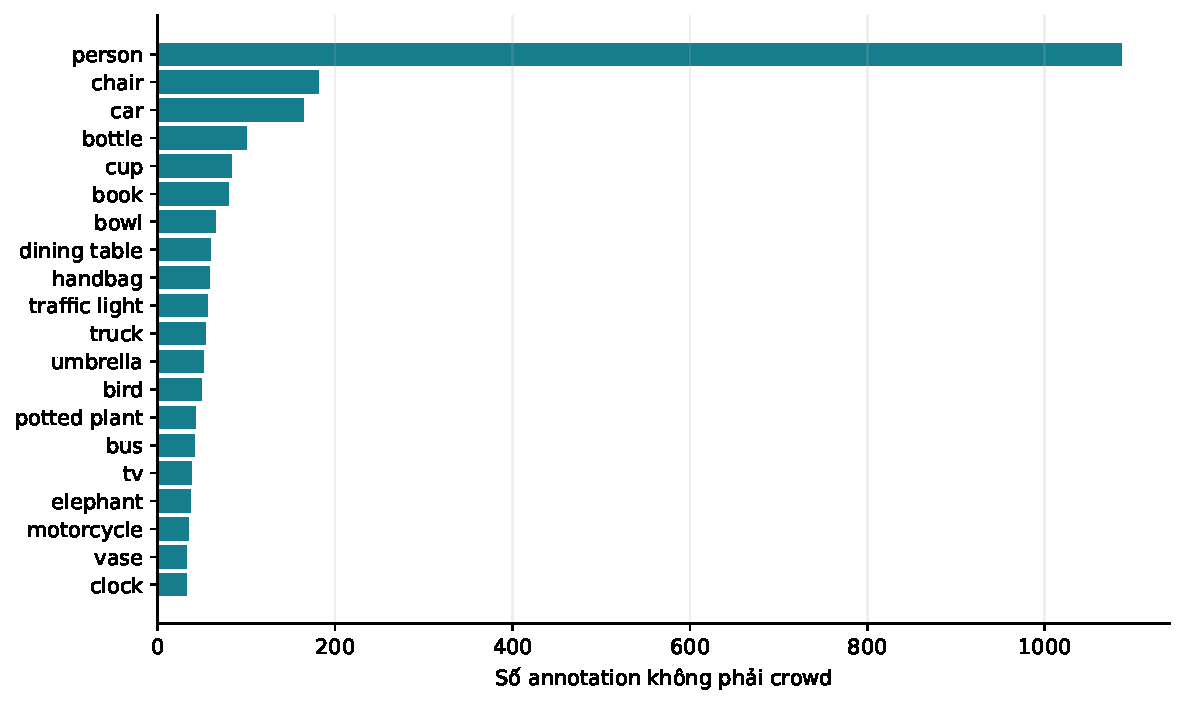
\includegraphics[width=0.94\textwidth]{klygo/distribution.pdf}
\caption{Hai mươi lớp có nhiều annotation không phải crowd nhất trong mẫu. Phân bố được tính trước khi xét dự đoán của mô hình.}
\label{fig:distribution}
\end{figure}
Lớp person có 1.087 annotation, chiếm khoảng 31,3\% trong tổng 3.475 ground truth hợp lệ, trong khi nhiều lớp còn lại có ít mẫu hơn đáng kể. Sự lệch phân bố làm cho P/R/F1 micro chịu ảnh hưởng mạnh từ các lớp phổ biến. AP trung bình theo lớp phân bổ trọng số khác, nên thứ tự mô hình theo một chỉ số không nhất thiết hoàn toàn giống theo chỉ số khác.

Các lớp ít annotation có độ nhạy cao đối với từng dự đoán đúng hoặc sai. Một lớp có AP cao trên vài vật thể không đủ để kết luận mô hình mạnh với lớp đó nói chung. Báo cáo cung cấp số GT theo lớp và bảng đầy đủ ở phụ lục để người đọc đánh giá mức hỗ trợ của mỗi nhận xét. Bộ COCO15 có trong dự án được xem là tài nguyên minh họa và kiểm thử tích hợp, không tham gia vào benchmark chính này.

\section{Môi trường và cấu hình mô hình}
\subsection{Phần cứng và phần mềm}
\begin{table}[H]\centering\small
\caption{Môi trường chạy thực nghiệm}
\begin{tabularx}{\textwidth}{p{5.1cm}Y}
\toprule Thành phần & Giá trị ghi nhận \\\midrule
Hệ điều hành & Windows, build 22631 \\
GPU & NVIDIA GeForce GTX 1650 Ti with Max-Q Design \\
VRAM / RAM hệ thống & Xấp xỉ 4 GiB / 31,73 GiB \\
Python / Klygo & 3.11.9 / 2.1.0 \\
PyTorch / Torchvision & 2.8.0+cu126 / 0.23.0+cu126 \\
CUDA runtime / Ultralytics & 12.6 / 8.3.228 \\
NumPy / Pillow / pycocotools & 2.2.6 / 11.3.0 / 2.0.10 \\
Độ chính xác số / batch & FP32 / 1 \\
Revision source & \code{0ca8a6a77600e1caf770ae8157d2df35360ee719} \\
\bottomrule
\end{tabularx}
\end{table}
CUDA được kiểm tra bằng phép tính tensor thực tế, không chỉ dựa trên việc tìm thấy tên GPU. Các model chạy lần lượt, mỗi lần giữ một model cho suy luận. Yếu tố xung nhịp, nhiệt độ và tải nền của máy không được khóa ở mức hệ điều hành; đây là một giới hạn khi diễn giải chênh lệch thời gian nhỏ.

\subsection{Checkpoint và tham số}
\begin{table}[H]\centering\small
\caption{Cấu hình model và hậu xử lý trong đánh giá chính}
\begin{tabularx}{\textwidth}{p{2.6cm}YY}
\toprule Cấu hình & Trọng số và backend & Tham số đáng chú ý \\\midrule
YOLOv8n & \code{yolov8n.pt}; Ultralytics & imgsz 640; conf 0,001; NMS IoU 0,7; max\_det 100 \\
YOLO-World v2 small & \code{yolov8s-worldv2.pt}; Ultralytics & Như YOLOv8n; vocabulary COCO của checkpoint \\
Faster R-CNN MobileNetV3-Large FPN & \code{COCO\_V1}; Torchvision & min\_size = max\_size = 640; score 0,001; NMS IoU 0,7; tối đa 100 box \\
\bottomrule
\end{tabularx}
\end{table}
Các ngưỡng số giống nhau không bảo đảm tác động giống nhau giữa các mô hình, vì confidence chưa được hiệu chuẩn chung và cấu trúc hậu xử lý khác nhau. Việc đặt min/max size cho Faster R-CNN cũng thay đổi cấu hình mặc định. Mục đích là công bố rõ một cấu hình giới hạn tài nguyên, không tái lập điểm model zoo hoặc chứng minh một họ kiến trúc luôn hơn họ khác.

Không áp dụng thêm một vòng NMS Klygo sau kết quả backend. Box chuyển sang định dạng COCO $xywh$, nhãn chuyển theo tên sang category ID gốc. AP được tính với confidence đầu vào thấp để giữ phần lớn đường cong PR. P/R/F1 được trích riêng tại confidence 0,25 và IoU 0,50, sử dụng quy tắc match/ignore của COCOeval.

\section{Kết quả kiểm thử thư viện}
\begin{table}[H]\centering\small
\caption{Phân bố 360 ca unittest theo nhóm; cột thực hiện bao gồm ca skip}
\begin{tabular}{lrrr}
\toprule
Nhóm & Thực hiện & Đạt & Bỏ qua \\
\midrule
archive & 50 & 50 & 0 \\
config & 24 & 24 & 0 \\
datasets & 34 & 34 & 0 \\
files & 85 & 85 & 0 \\
integration & 4 & 1 & 3 \\
media & 8 & 8 & 0 \\
models & 76 & 72 & 4 \\
outputs & 28 & 28 & 0 \\
postprocessing & 7 & 7 & 0 \\
preprocessing & 12 & 12 & 0 \\
test\_cross\_modules & 1 & 1 & 0 \\
test\_e2e\_zero\_ram & 1 & 1 & 0 \\
test\_path\_conventions & 2 & 2 & 0 \\
test\_public\_api & 4 & 4 & 0 \\
test\_public\_imports & 3 & 3 & 0 \\
utils & 11 & 11 & 0 \\
validators & 6 & 6 & 0 \\
visual & 4 & 4 & 0 \\
\bottomrule
\end{tabular}

\label{tab:tests}
\end{table}
Tổng cộng 353 ca đạt, 7 ca bỏ qua, không có fail hoặc error sau khi đủ phụ thuộc. Ba ca skip thuộc quy trình COCO15 cần dataset và bundle đã sinh; bốn ca opt-in cần đường dẫn checkpoint thật cho YOLO, YOLO-World, Grounding DINO và Locate Anything. Hai mô hình YOLO đã được chạy thật qua mã thực nghiệm báo cáo, nhưng các ca opt-in tương ứng trong unittest vẫn được ghi đúng là skip vì không cấu hình biến môi trường của chúng.

Công cụ audit cả 12 mô-đun cũng hoàn tất với trạng thái đạt đối với source, tài liệu, ví dụ và hợp đồng notebook. Các kiểm tra này hỗ trợ RQ1 và RQ2 ở mức phần mềm. Chúng không chứng minh mọi backend đã chạy trên mọi loại phần cứng, và không suy ra tỷ lệ nhận dạng đúng ngoài dữ liệu đánh giá.

\section{Chất lượng phát hiện trên 500 ảnh}
\subsection{AP tổng hợp và precision--recall}
\begin{table}[H]\centering
\caption{Chất lượng phát hiện sau pipeline Klygo trên cùng 500 ảnh; điểm tính theo phần trăm}
\begin{tabular}{lrrr}
\toprule
Mô hình & AP (\%) & AP50 (\%) & AP75 (\%) \\
\midrule
YOLOv8n & 38{,}24 & 52{,}55 & 41{,}66 \\
YOLO-World & 39{,}07 & 53{,}23 & 42{,}41 \\
Faster R-CNN & 25{,}08 & 39{,}49 & 26{,}31 \\
\bottomrule
\end{tabular}

\label{tab:quality}
\end{table}
YOLO-World có AP cao nhất trong ba cấu hình được đo, hơn YOLOv8n khoảng 0,82 điểm phần trăm. Chênh lệch này nhỏ so với sự khác nhau giữa từng lớp, nên chưa đủ để kết luận ưu thế ổn định trên dữ liệu khác. Faster R-CNN thấp hơn trong cấu hình khảo sát; kết quả gắn với checkpoint MobileNetV3, chính sách resize và ngưỡng cụ thể, không đại diện cho mọi mô hình hai giai đoạn.

AP50 của cả ba đều cao hơn AP75, phù hợp với việc ngưỡng IoU chặt hơn đòi hỏi box chính xác hơn. Điều này gợi ý cần phân tích cả định vị thay vì chỉ nhìn số đối tượng được gán đúng tên. Tuy nhiên, khoảng cách AP50--AP75 không tách riêng hoàn toàn lỗi định vị khỏi các yếu tố khác của đường cong PR, nên không được diễn giải thành tỷ lệ chính xác của một loại lỗi duy nhất.

\begin{figure}[H]\centering
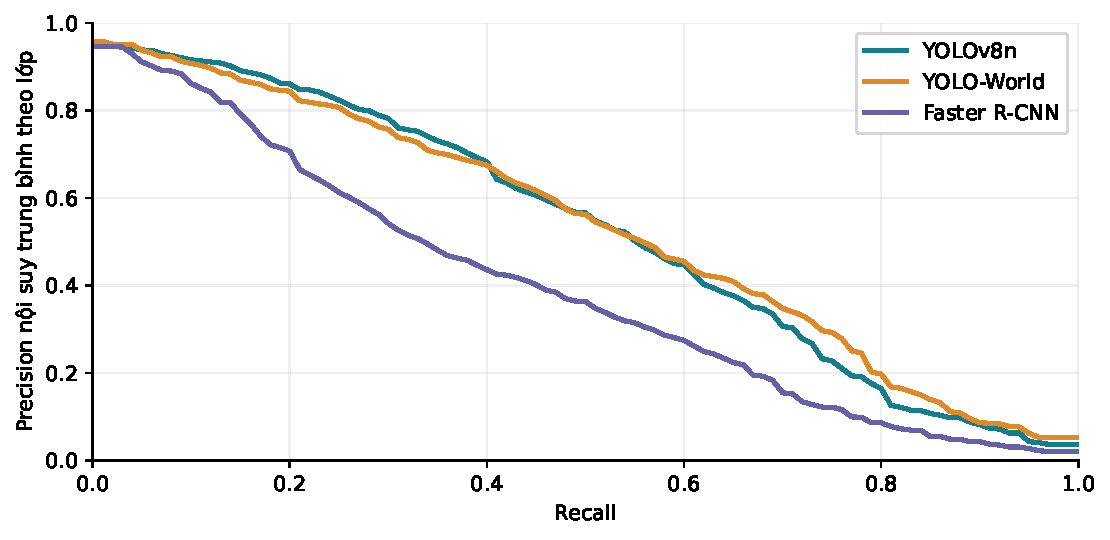
\includegraphics[width=0.94\textwidth]{klygo/pr.pdf}
\caption{Precision nội suy trung bình theo lớp tại IoU 0,50. Đây là đường macro từ COCOeval, khác P/R micro ở một điểm confidence.}
\label{fig:pr}
\end{figure}
Đường cong cho thấy precision giảm khi yêu cầu đạt recall cao hơn. Nó giúp nhìn rộng hơn một điểm confidence 0,25 và thể hiện mức mất precision để tăng độ bao phủ. Phần đuôi đường cong chịu ảnh hưởng số dự đoán tối đa, score threshold, các vật thể khó và khả năng nhận dạng. Do score đã được làm tròn trong builder, các nhóm dự đoán đồng hạng còn có thể tác động đến thứ tự tích lũy; đây là đặc điểm của pipeline đã đánh giá.

\subsection{Điểm làm việc tại confidence 0,25}
\begin{table}[H]\centering\small
\caption{Số đếm và P/R/F1 micro tại confidence 0,25, IoU 0,50}
\begin{tabular}{lrrrrrr}
\toprule
Mô hình & TP & FP & FN & P & R & F1 \\
\midrule
YOLOv8n & 1752 & 695 & 1723 & 0{,}7160 & 0{,}5042 & 0{,}5917 \\
YOLO-World & 1895 & 1003 & 1580 & 0{,}6539 & 0{,}5453 & 0{,}5947 \\
Faster R-CNN & 1574 & 3258 & 1901 & 0{,}3257 & 0{,}4529 & 0{,}3790 \\
\bottomrule
\end{tabular}

\label{tab:operating}
\end{table}
YOLOv8n có Precision khoảng 0,716 và Recall khoảng 0,504. YOLO-World tìm được thêm 143 TP so với YOLOv8n, đồng thời có thêm 308 FP; vì vậy Recall cao hơn nhưng Precision thấp hơn tại cùng ngưỡng. F1 của hai cấu hình gần nhau, khoảng 0,592 và 0,595. Những con số này minh họa vì sao một thay đổi về số TP không thể được đánh giá tách khỏi số FP và FN.

Faster R-CNN tạo nhiều FP hơn tại điểm làm việc đã chọn. Không thể từ đó kết luận confidence 0,25 có cùng ý nghĩa xác suất cho cả ba model. Trong một ứng dụng triển khai, người dùng có thể hiệu chuẩn hoặc chọn ngưỡng theo chi phí lỗi trên một tập phát triển riêng. Báo cáo không thực hiện bước tối ưu đó trên chính tập đánh giá, vì làm như vậy sẽ làm thay đổi cách diễn giải kết quả kiểm chứng.

\subsection{Kết quả theo kích thước vật thể}
\begin{table}[H]\centering
\caption{AP theo các nhóm kích thước của COCOeval}
\begin{tabular}{lrrr}
\toprule
Mô hình & AP small (\%) & AP medium (\%) & AP large (\%) \\
\midrule
YOLOv8n & 21{,}75 & 44{,}43 & 56{,}53 \\
YOLO-World & 26{,}21 & 43{,}44 & 55{,}41 \\
Faster R-CNN & 5{,}51 & 29{,}04 & 51{,}84 \\
\bottomrule
\end{tabular}

\label{tab:sizeap}
\end{table}
Trong mẫu này, nhóm small khó hơn rõ rệt ở cả ba mô hình. YOLO-World có AP small 26,21\%, cao hơn 21,75\% của YOLOv8n, trong khi Faster R-CNN chỉ đạt 5,51\% theo cấu hình giới hạn kích thước đang dùng. Ở nhóm large, khoảng cách giữa các mô hình thu hẹp. Kết quả phù hợp với nhu cầu giữ chi tiết ảnh khi phát hiện vật thể nhỏ, nhưng không đủ xác định riêng resize là nguyên nhân của mọi sai khác.

COCOeval phân nhóm bằng diện tích annotation gốc, không bằng cách tự so kích thước box dự đoán với một ngưỡng pixel sau resize. Một lớp có thể có mặt trong nhóm large mà không có ground truth trong nhóm small. Vì vậy, các AP theo kích thước có thể được trung bình trên các tập lớp hợp lệ khác nhau; chúng cần được xem cùng quy mô dữ liệu, không như ba bài toán có cùng phân bố hoàn toàn.

\subsection{Khác biệt theo lớp}
\begin{table}[H]\centering\small
\caption{AP theo lớp của 12 lớp nhiều GT nhất; các cột mô hình là AP tính bằng phần trăm}
\begin{tabular}{lrrrr}
\toprule
Lớp & GT hợp lệ & YOLOv8n & YOLO-World & Faster R-CNN \\
\midrule
person & 1087 & 51{,}20 & 54{,}55 & 32{,}48 \\
chair & 181 & 29{,}19 & 30{,}86 & 15{,}20 \\
car & 164 & 33{,}08 & 37{,}25 & 17{,}54 \\
bottle & 100 & 31{,}59 & 41{,}43 & 16{,}33 \\
cup & 83 & 41{,}46 & 46{,}58 & 17{,}59 \\
book & 80 & 11{,}84 & 11{,}68 & 2{,}27 \\
bowl & 65 & 40{,}38 & 45{,}70 & 21{,}30 \\
dining table & 59 & 27{,}34 & 27{,}03 & 17{,}91 \\
handbag & 58 & 11{,}14 & 20{,}04 & 3{,}23 \\
traffic light & 56 & 19{,}75 & 15{,}15 & 10{,}49 \\
truck & 54 & 26{,}40 & 28{,}14 & 15{,}53 \\
umbrella & 52 & 46{,}14 & 45{,}67 & 26{,}39 \\
\bottomrule
\end{tabular}

\label{tab:classes}
\end{table}
Các lớp trong bảng được chọn theo số ground truth, không theo việc mô hình nào có điểm cao. Person có AP cao hơn book và handbag đối với cả ba cấu hình. Điều này cho thấy điểm tổng hợp che khuất nhiều khác biệt giữa các nhóm vật thể. Đặc biệt, book có 80 annotation nhưng AP chỉ khoảng 11,8\% đối với hai biến thể YOLO, nên không thể giải thích mọi điểm thấp chỉ bằng thiếu mẫu.

YOLO-World không cao hơn YOLOv8n trên mọi lớp: traffic light, dining table và umbrella trong bảng có các mức chênh lệch khác nhau. Những kết quả này củng cố cách chọn mô hình theo tập lớp và mục tiêu ứng dụng thay vì chỉ lấy một AP tổng hợp. Các lớp ít mẫu và lớp không có GT được giữ trong bảng đầy đủ ở phụ lục, với ký hiệu không áp dụng khi metric không xác định.

\section{Độ trễ và sự đánh đổi chất lượng--thời gian}
\subsection{Thiết kế phép đo}
Một trăm ảnh đầu theo thứ tự manifest được nạp thành ảnh RGB trong RAM. Mỗi model warm-up năm lần, sau đó đo ba lượt trên cùng 100 ảnh. Các nhánh đều batch bằng một, FP32, inference mode và có CUDA synchronize trước/sau timer. Tải mạng, đọc ảnh từ đĩa và nạp checkpoint nằm ngoài vùng đo. Model được đánh giá lần lượt trên một GPU.

\begin{table}[H]\centering
\caption{Thời gian predict trên 100 ảnh, ba lượt; 300 lần gọi mỗi model}
\begin{tabular}{lrrrr}
\toprule
Mô hình & TB (ms) & Trung vị & p90 & FPS tuần tự \\
\midrule
YOLOv8n & 27{,}02 & 28{,}32 & 30{,}92 & 37{,}01 \\
YOLO-World & 32{,}46 & 34{,}13 & 36{,}24 & 30{,}81 \\
Faster R-CNN & 61{,}54 & 55{,}37 & 88{,}47 & 16{,}25 \\
\bottomrule
\end{tabular}

\label{tab:latency}
\end{table}
YOLOv8n có độ trễ trung bình thấp nhất trong cấu hình đo. YOLO-World mất thêm khoảng 5,44 ms nhưng có AP cao hơn khoảng 0,82 điểm phần trăm trên mẫu chất lượng. Faster R-CNN chậm hơn và có điểm thấp hơn trong lần khảo sát này. Các so sánh chỉ phản ánh cấu hình end-to-end qua Klygo; chúng không tách độc lập đóng góp của backbone, backend, preprocessing và output conversion.

\begin{figure}[H]\centering
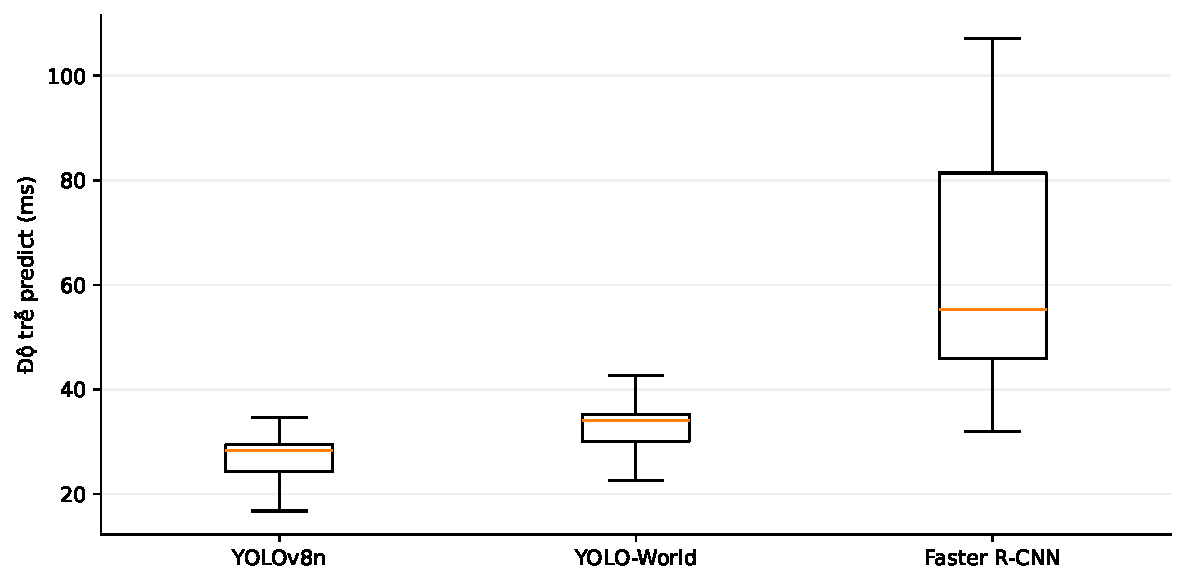
\includegraphics[width=0.94\textwidth]{klygo/latency.pdf}
\caption{Phân bố độ trễ predict qua 300 lần gọi mỗi model. Boxplot lược điểm ngoại lai khi vẽ; tệp latency vẫn giữ toàn bộ mẫu.}
\label{fig:latency}
\end{figure}
Trung vị Faster R-CNN thấp hơn trung bình và p90 lớn hơn đáng kể, cho thấy thời gian không có phân bố đối xứng đơn giản. Sự khác biệt kích thước/tỷ lệ ảnh, số box và công việc hậu xử lý có thể cùng góp phần vào biến thiên. Đề tài chưa thực hiện phân rã timer theo từng thành phần nên không gán một nguyên nhân duy nhất cho các lần gọi chậm.

\begin{table}[H]\centering
\caption{Độ trễ predict trung bình theo từng lượt lặp}
\begin{tabular}{lrrr}
\toprule
Mô hình & Lượt 1 (ms) & Lượt 2 (ms) & Lượt 3 (ms) \\
\midrule
YOLOv8n & 27{,}51 & 27{,}14 & 26{,}40 \\
YOLO-World & 33{,}09 & 31{,}96 & 32{,}32 \\
Faster R-CNN & 61{,}81 & 61{,}29 & 61{,}52 \\
\bottomrule
\end{tabular}

\end{table}
Các lượt dùng lại cùng ảnh, nên có thể phản ánh biến thiên do tải máy, cache hoặc xung nhịp. Ba lượt không biến 100 ảnh thành 300 ảnh độc lập để đánh giá tổng quát hóa. FPS trong Bảng~\ref{tab:latency} được suy từ thời gian trung bình tuần tự, không phải tốc độ tối đa của hệ thống xử lý video có pipeline hoặc batching.

\begin{figure}[H]\centering
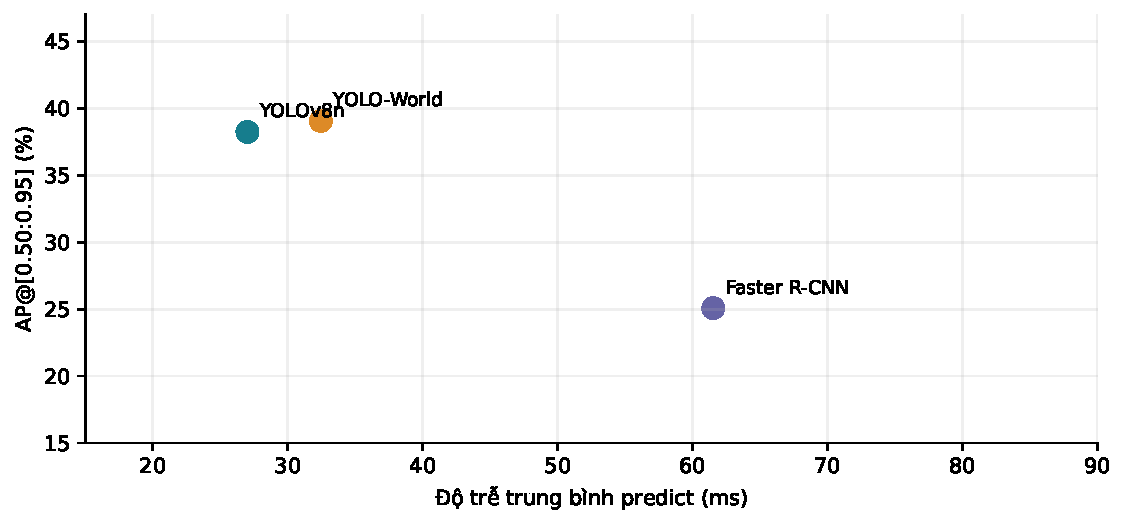
\includegraphics[width=0.94\textwidth]{klygo/tradeoff.pdf}
\caption{Chất lượng trên 500 ảnh và độ trễ lặp trên 100 ảnh. Mỗi điểm biểu diễn một cấu hình hệ thống, không phải một phép đo riêng của backend.}
\label{fig:tradeoff}
\end{figure}

\subsection{Chi phí của lớp điều phối predict}
Để trả lời RQ4, mã gọi cùng model theo hai cách: trực tiếp \code{forward([image])} trả frame \code{Detection}, và \code{predict(image)} tạo kết quả có điều phối nguồn, cấu hình, metadata và collection. Cả hai giữ preprocessing, inference, hậu xử lý backend và đóng gói Detection. Vì baseline vẫn sử dụng adapter và kiểu đầu ra Klygo, phép đo chỉ tách chi phí lifecycle của predict; nó không đo toàn bộ chi phí Klygo so với một framework thuần.

\begin{table}[H]\centering\small
\caption{Đo cặp predict và forward với cùng inference mode và đầu ra tương đương}
\begin{tabular}{lrrrr}
\toprule
Mô hình & forward (ms) & predict (ms) & $\Delta$ (ms) & $\Delta$ (\%) \\
\midrule
YOLOv8n & 24{,}53 & 27{,}02 & 2{,}49 & 10{,}15 \\
YOLO-World & 29{,}98 & 32{,}46 & 2{,}48 & 8{,}28 \\
Faster R-CNN & 59{,}16 & 61{,}54 & 2{,}38 & 4{,}03 \\
\bottomrule
\end{tabular}

\label{tab:overhead}
\end{table}
Mỗi mô hình có 300 cặp đo, đổi thứ tự nhánh theo ảnh và lượt. Không có cặp nào khác về số box, nhãn, tọa độ hoặc score vượt sai số cho phép. Chênh lệch trung bình khoảng 2,38--2,49 ms, tương ứng khoảng 4,03--10,15\% của baseline forward. Tỷ lệ tương đối của YOLOv8n lớn hơn vì thời gian nền của nó thấp hơn; không có nghĩa lớp điều phối phải thực hiện một lượng công việc gấp đôi cho model đó.

\begin{figure}[H]\centering
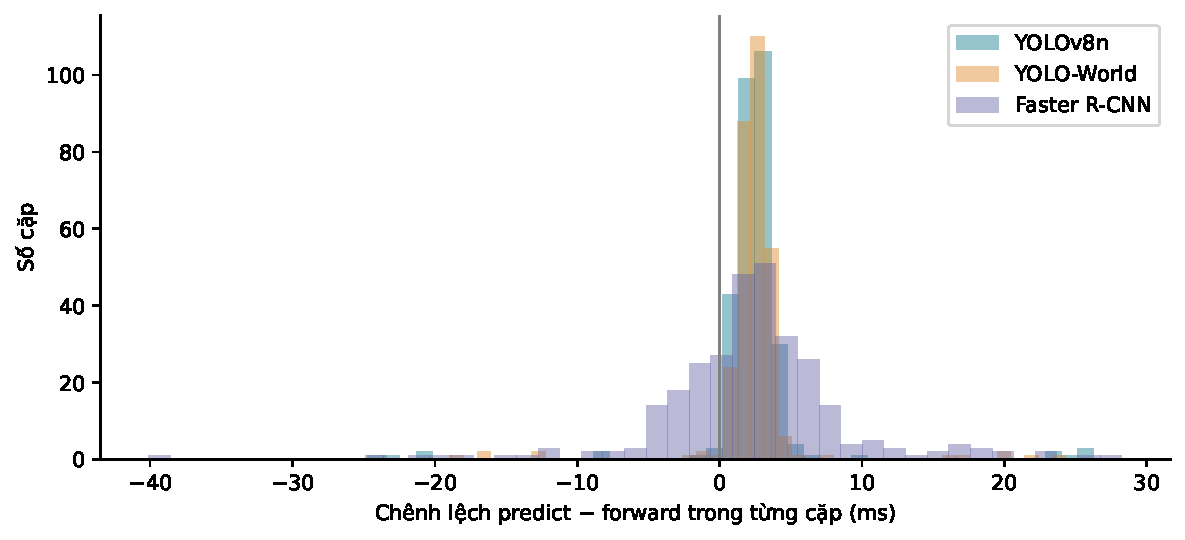
\includegraphics[width=0.94\textwidth]{klygo/overhead.pdf}
\caption{Phân bố chênh lệch trong từng cặp thời gian. Chênh lệch âm riêng lẻ được giữ lại như biến thiên đo, không bị cắt về không.}
\end{figure}
Các cặp chậm hoặc chênh lệch âm có thể xuất hiện vì hai lời gọi không chạy tại cùng một thời điểm tuyệt đối. Vì thế, chênh lệch không nên được xem là hằng số chính xác của mọi lần gọi. Kết quả hỗ trợ một nhận xét có phạm vi: trên nguồn PIL đã sẵn trong RAM và batch một, lớp điều phối bổ sung vài mili giây trong ba cấu hình được đo. Tình huống video, ảnh lazy chưa giải mã, batch lớn hoặc nhiều luồng cần đo lại.

\section{Phân tích trường hợp thành công và lỗi}
Ba ảnh được chọn bằng quy tắc công bố: ảnh tốt có F1 YOLOv8n cao nhất trong nhóm ít nhất ba GT hợp lệ; ảnh khó có tổng FP+FN YOLOv8n lớn nhất trong cùng nhóm; ảnh small có nhiều annotation small nhất sau khi loại hai ảnh trước. Tiêu chí sử dụng YOLOv8n làm điểm chọn ảnh, nên đây là phân tích trường hợp có chủ đích, không phải một ước lượng trung lập về phân bố lỗi của toàn bộ mô hình.

Ảnh ID 67406 có bốn ground truth hợp lệ. Hai mô hình YOLO đều đạt bốn TP, không FP tại điểm làm việc; Faster R-CNN có bốn TP nhưng thêm sáu FP. Trường hợp này cho thấy việc tìm đủ vật thể vẫn có thể đi kèm kết quả dư thừa. Ảnh ID 65288 là một cảnh có nhiều đối tượng, che khuất và khác biệt tỷ lệ: 37 GT hợp lệ nhưng chỉ có 6, 10 và 6 TP tương ứng. Ảnh ID 432898 có 35 GT hợp lệ và nhiều vật thể nhỏ; Faster R-CNN có 11 TP nhưng 46 FP tại ngưỡng đã chọn.

\begin{figure}[H]\centering\includegraphics[width=\textwidth]{klygo/case_good.png}
\caption[So sánh kết quả trên ảnh COCO ID 67406]{Ảnh COCO ID 67406; tiêu chí chọn: F1 cao nhất của YOLOv8n trong các ảnh có ít nhất ba GT hợp lệ. Dự đoán hiển thị tại confidence 0,25; chỉ vẽ tối đa 20 box và lược nhãn trên ảnh để tránh che khuất. Số box trong tiêu đề là số trước giới hạn hiển thị. Metric dùng toàn bộ dự đoán theo cấu hình.}\label{fig:case-good}
\end{figure}

\begin{figure}[H]\centering\includegraphics[width=\textwidth]{klygo/case_hard.png}
\caption[So sánh kết quả trên ảnh COCO ID 65288]{Ảnh COCO ID 65288; tiêu chí chọn: tổng FP và FN lớn nhất của YOLOv8n trong các ảnh có ít nhất ba GT hợp lệ. Dự đoán hiển thị tại confidence 0,25; chỉ vẽ tối đa 20 box và lược nhãn trên ảnh để tránh che khuất. Số box trong tiêu đề là số trước giới hạn hiển thị. Metric dùng toàn bộ dự đoán theo cấu hình.}\label{fig:case-hard}
\end{figure}

\begin{figure}[H]\centering\includegraphics[width=\textwidth]{klygo/case_small.png}
\caption[So sánh kết quả trên ảnh COCO ID 432898]{Ảnh COCO ID 432898; tiêu chí chọn: số annotation small nhiều nhất, sau khi loại hai ảnh đã chọn. Dự đoán hiển thị tại confidence 0,25; chỉ vẽ tối đa 20 box và lược nhãn trên ảnh để tránh che khuất. Số box trong tiêu đề là số trước giới hạn hiển thị. Metric dùng toàn bộ dự đoán theo cấu hình.}\label{fig:case-small}
\end{figure}

Các panel giữ vị trí ảnh giống nhau giữa ground truth và model. Để hình không bị che bởi nhãn chồng lấn, chỉ vẽ tối đa 20 box và không in nhãn lên từng box trong montage. Dữ liệu định lượng sử dụng toàn bộ dự đoán đã lưu. Một box dự đoán có vẻ nằm gần vật thể khi nhìn ảnh vẫn có thể là FP nếu không đúng lớp hoặc chưa đạt IoU 0,50; các số đếm được xác định bằng quy tắc ghép, không bằng nhận xét bằng mắt.

Từ ba trường hợp có thể đặt ra hướng khảo sát tiếp theo: kiểm tra ảnh dày vật thể và che khuất, tăng độ phân giải cho nhóm small, hoặc điều chỉnh ngưỡng theo yêu cầu giảm FP trên một tập phát triển riêng. Những hướng này là giả thuyết cần thử nghiệm thêm; số liệu hiện tại chưa đủ chứng minh một thay đổi cụ thể sẽ cải thiện đồng thời mọi chỉ số.

\section{Giới hạn và các mối đe dọa tới tính hợp lệ}
\textbf{Giới hạn về dữ liệu.} Mẫu 500 ảnh chỉ là một phần validation. Các lớp hiếm có số mẫu thấp và một lớp không có GT hợp lệ, làm điểm theo lớp không ổn định. Các checkpoint được huấn luyện hoặc tiền huấn luyện trên các dữ liệu do tác giả công bố; báo cáo không chứng minh toàn bộ dữ liệu tiền huấn luyện độc lập với mọi ảnh/khái niệm trong mẫu. Do đó không dùng kết quả này để khẳng định zero-shot trên lớp mới.

\textbf{Giới hạn về cấu hình.} Các model dùng chính sách resize khác nhau, score chưa được hiệu chuẩn chung và Faster R-CNN đã thay đổi min/max size so với mặc định. Kết quả là so sánh các cấu hình triển khai cụ thể. Builder Klygo làm tròn dữ liệu, nên AP có thể khác kết quả tính từ tensor gốc. Thí nghiệm chưa đo riêng ảnh hưởng của làm tròn hoặc resize.

\textbf{Giới hạn về hiệu năng.} Chỉ dùng một máy và một GPU, không khóa xung nhịp, nhiệt độ hoặc tải nền. Thời gian không bao gồm mạng, đọc đĩa, hiển thị và nạp checkpoint. Độ trễ thấp trong phép đo không chứng minh hệ thống phục vụ thời gian thực cho một ứng dụng có thêm nhiều bước khác.

\textbf{Giới hạn về suy luận thống kê.} Báo cáo công bố điểm và các lượt lặp thời gian, chưa cung cấp khoảng tin cậy bootstrap cho chênh lệch AP. Chênh lệch 0,82 điểm phần trăm giữa hai biến thể YOLO vì vậy được xem là kết quả quan sát trên mẫu cố định, không phải khẳng định có ý nghĩa thống kê. Tính tương đương của hai nhánh thời gian được kiểm tra trên dữ liệu đo, không phải chứng minh cho mọi đầu vào có thể có.

\textbf{Giới hạn về phạm vi sản phẩm.} Kiểm thử giả lập không thay thế checkpoint thật; khả năng có mã adapter không đồng nghĩa mọi backend đã được xác nhận trong báo cáo. Grounding DINO, Locate Anything và KerasHub chưa tham gia phép đo chính. Khả năng streaming có kiểm thử hợp đồng, nhưng chưa có benchmark bộ nhớ dài hạn hay thử tải nhiều người dùng.

\section{Thực nghiệm mining và kiểm chứng dữ liệu xuất}
\label{sec:mining-exp}
Thực nghiệm mở rộng dùng revision \code{c4388f1}. Từ thứ tự 500 ID đã cố định trong manifest, 300 ảnh đầu làm tập tuyển chọn/train, 100 ảnh tiếp theo làm validation và 100 ảnh cuối làm test. Đây là phép chia phục vụ nghiên cứu nhỏ trên COCO val2017, không phải tập train/test chính thức của COCO. Các số AP của ba checkpoint ở phần trước vẫn được tính trên đủ 500 ảnh với checkpoint chưa fine-tune; các checkpoint fine-tune không được đánh giá lại trên những ảnh đã dùng train để báo kết quả tổng quát hóa.

Mining chỉ truy cập tập train. Annotation crowd bị loại khỏi bộ YOLO của thí nghiệm; box được chặn trong biên ảnh và chỉ giữ diện tích dương. Tập tuyển chọn có 300 ảnh và 2.099 box. Ba tập được tách bằng ID ảnh; nghiên cứu chưa bổ sung loại trùng ngữ nghĩa hoặc nhóm ảnh gần giống giữa các split. Không sử dụng nhãn tự động.

Random, Weighted, Diversity và Rare-first có ngân sách 150 ảnh. Diversity dùng 150 cụm và chọn một đại diện mỗi cụm; seed chọn bằng 42. Quality dùng ngưỡng 0,5; Boxes yêu cầu ít nhất hai box; Class yêu cầu có lớp person; Quota và Coverage đặt quota ba ảnh/lớp với giới hạn 150; Balance dùng median theo số ảnh chứa lớp. Các bộ lọc và quota có thể trả ít hơn giới hạn nên không được xem là đối chứng cùng ngân sách cho mọi hàng.

Thời gian chọn lấy trung vị ba lần sau một lượt warm-up trên collection đã nạp, chạy CPU. Weighted và Diversity bao gồm tính điểm hoặc trích đặc trưng/phân cụm trong mỗi lần đo; không dùng báo cáo tính sẵn để che chi phí chuẩn bị. Thời gian không gồm export. Hàng full chỉ tham chiếu collection đầu vào nên thời gian gần bằng không, không phải chi phí đọc dữ liệu từ đĩa.

\begin{table}[H]\centering\small
\caption{Benchmark tuyển chọn trên 300 ảnh; IR chỉ tính các lớp hiện diện}
\begin{tabular}{lrrrrr}
\toprule
Cách chọn & Ảnh & Box & Lớp & IR & Chọn (ms) \\
\midrule
full & 300 & 2099 & 77 & 167.0 & 0.0 \\
random & 150 & 1070 & 76 & 79.0 & 9.3 \\
weighted & 150 & 1410 & 77 & 69.0 & 4693.7 \\
diversity & 150 & 1172 & 75 & 87.0 & 5980.4 \\
rare-first & 150 & 904 & 76 & 42.0 & 4337.5 \\
coverage & 97 & 835 & 77 & 45.0 & 130.2 \\
quota & 97 & 835 & 77 & 45.0 & 93.7 \\
quality & 150 & 1160 & 74 & 91.0 & 4374.7 \\
boxes & 150 & 1266 & 74 & 92.0 & 10.0 \\
class & 150 & 1321 & 69 & 150.0 & 9.2 \\
balance & 212 & 1553 & 77 & 111.0 & 141.0 \\
\bottomrule
\end{tabular}

\end{table}
Quota và Coverage tạo cùng tập ảnh do đi qua cùng hàm greedy; chênh lệch thời gian đo không phải bằng chứng khác biệt thuật toán. Balance có thể giữ hơn 150 ảnh và không bị áp cùng ngân sách. Weighted giữ nhiều box hơn Random dù số ảnh bằng nhau, nên thực nghiệm huấn luyện cùng số ảnh chưa phải cùng số đối tượng được quan sát. Khi đánh giá hiệu quả chọn cần công bố cả hai đơn vị.

\begin{figure}[H]\centering
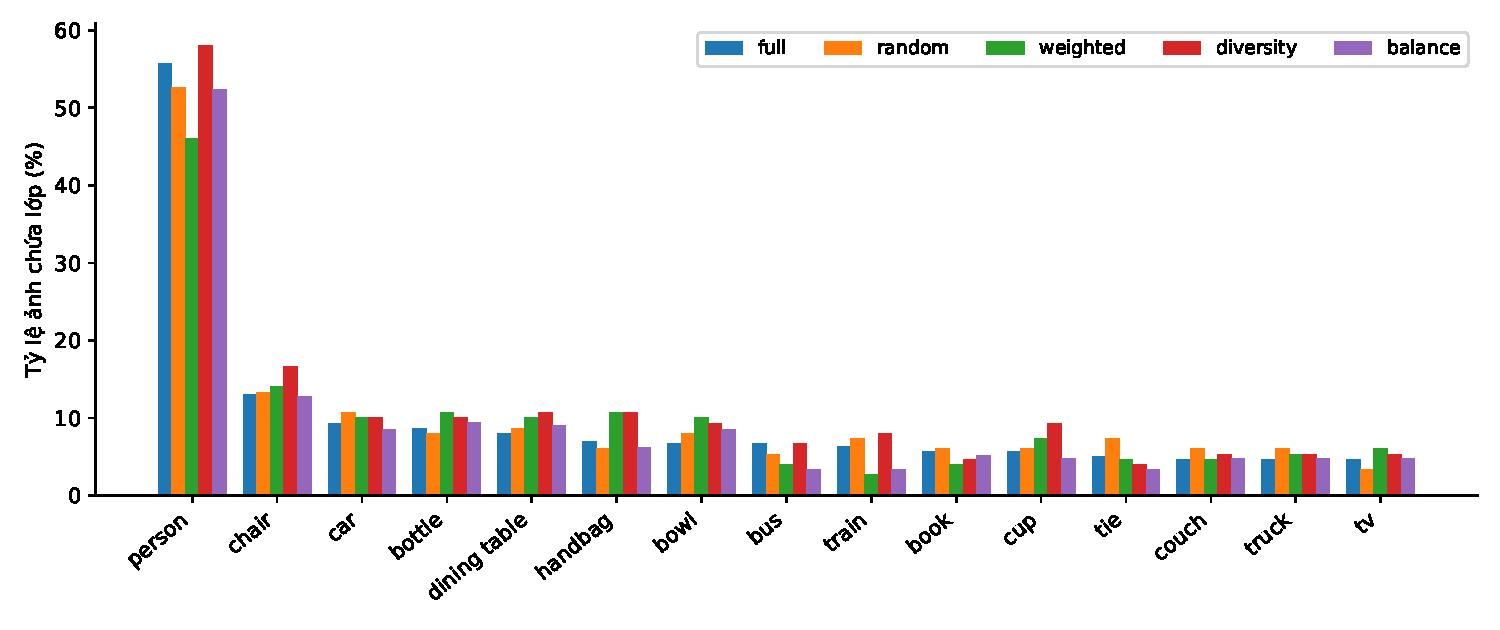
\includegraphics[width=\textwidth]{klygo/mining_distribution.pdf}
\caption{Phân bố 15 lớp phổ biến nhất của tập đầu vào, chuẩn hóa theo số ảnh của từng tập}
\end{figure}
\begin{figure}[H]\centering
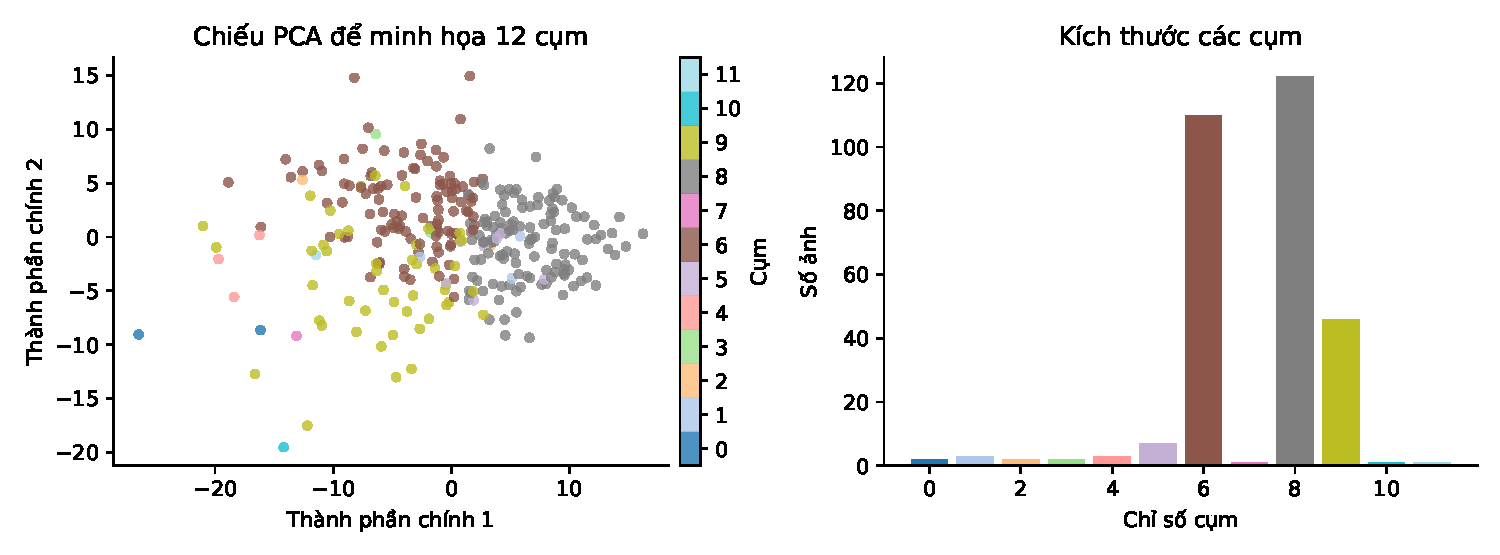
\includegraphics[width=\textwidth]{klygo/mining_clusters.pdf}
\caption{Minh họa 12 cụm trên 300 ảnh; PCA chỉ dùng để vẽ, không dùng để chọn mẫu}
\end{figure}
Hình phân cụm dùng $K=12$ để quan sát và được lưu riêng với cấu hình tuyển chọn $K=150$. Phân tích thành phần chính (PCA) chiếu dữ liệu lên hai hướng có phương sai lớn để minh họa. Khoảng cách trên mặt phẳng này không bảo toàn toàn bộ khoảng cách 726 chiều; ảnh gần nhau trên hình chưa đủ để kết luận là ảnh trùng. Không lựa chọn $K$ hay trọng số dựa trên điểm test.

\subsection{Từ export annotation đến bộ dữ liệu huấn luyện}
Trong revision này, \code{Detections.export(format="yolo")} ghi nhãn, registry lớp và manifest, không sao chép ảnh nguồn. Script thực nghiệm ghép ảnh theo \code{source\_path}, đổi tên tương ứng \code{label\_file}, rồi tạo YAML với đường dẫn train/val/test. Việc ghép ảnh và tạo YAML là bước chuẩn bị bổ sung của thực nghiệm, không được quy cho API export tự thực hiện.

Mỗi phương pháp được kiểm tra số ID duy nhất, tập ID là tập con của train, số ảnh/box và số box theo từng lớp sau khi đọc lại bằng \code{datasets.load}. Các kiểm tra đều đạt; nội dung đầu vào được đối chiếu trước và sau mining để xác nhận không bị thay đổi. Kiểm tra round-trip này xác nhận tính toàn vẹn cấu trúc và số nhãn, không thay thế đánh giá chất lượng annotation.

Export đánh lại class ID liên tục theo registry hiện diện của từng tập. Vì các tập có thể thiếu những lớp khác nhau, bộ nhãn được ánh xạ lại theo tên về cùng thứ tự 80 lớp COCO trước khi train. Script \code{prepare\_training\_canonical.py} kiểm tra bảo toàn số box theo tên lớp sau phép đổi ID. Lượt thử trước khi phát hiện khác biệt registry đã được dừng và giữ riêng; chỉ kết quả trong \code{training\_canonical} được dùng ở bảng và biểu đồ huấn luyện.

\section{Fine-tune trên dữ liệu được tuyển chọn}
\label{sec:mining-train}
Bốn cấu hình train là Full (300 ảnh), Random, Weighted và Diversity (mỗi tập 150 ảnh). Mọi lượt bắt đầu từ cùng checkpoint YOLOv8n COCO pretrained. Mỗi cấu hình chạy năm epoch với ba seed huấn luyện 42, 43 và 44; tập được chọn giữ nguyên seed 42. Độ lệch chuẩn vì vậy mô tả biến thiên huấn luyện có điều kiện trên các tập đã cố định, chưa bao gồm biến thiên khi chọn lại dữ liệu.

Vocabulary của model và YAML được giữ đủ 80 lớp để đầu ra có ý nghĩa nhất quán và sử dụng nguyên checkpoint khởi tạo. Tập full train có 77 lớp hiện diện; số lớp có ground truth trong test là 73. Các lớp ít mẫu khiến AP nhạy với một vài dự đoán; không diễn giải trung bình trên tập test nhỏ như mức chất lượng của toàn bộ COCO.

Thiết lập gồm kích thước 320, batch tám, FP32, AdamW, learning rate đầu 0,001, hệ số cuối 0,1, không warm-up, không mosaic/mixup và không early stopping. Số worker đọc dữ liệu bằng không. Sử dụng checkpoint epoch cuối, không chọn checkpoint theo tập test. Chất lượng được đo bằng metric bbox của Ultralytics trên 100 ảnh test, confidence 0,001, NMS IoU 0,7, max detections 100. Quy trình huấn luyện và tham số được lưu kèm \citep{ultralyticsTrain}; phiên bản thực thi được khóa ở 8.3.228. AP ở mục này không trộn với kết quả COCOeval 500 ảnh/kích thước 640 ở phần trước.

\begin{table}[H]\centering\small
\caption{Fine-tune năm epoch: trung bình và độ lệch chuẩn mẫu qua ba seed}
\begin{tabular}{lrrrr}
\toprule
Tập train & Ảnh & AP (\%) & AP50 (\%) & Train (s) \\
\midrule
full & 300 & 10.38 $\pm$ 1.91 & 17.28 & 52.4 \\
random & 150 & 10.10 $\pm$ 0.61 & 16.20 & 30.4 \\
weighted & 150 & 10.38 $\pm$ 0.55 & 16.83 & 30.7 \\
diversity & 150 & 8.00 $\pm$ 1.85 & 14.14 & 30.6 \\
\bottomrule
\end{tabular}

\end{table}
\begin{figure}[H]\centering
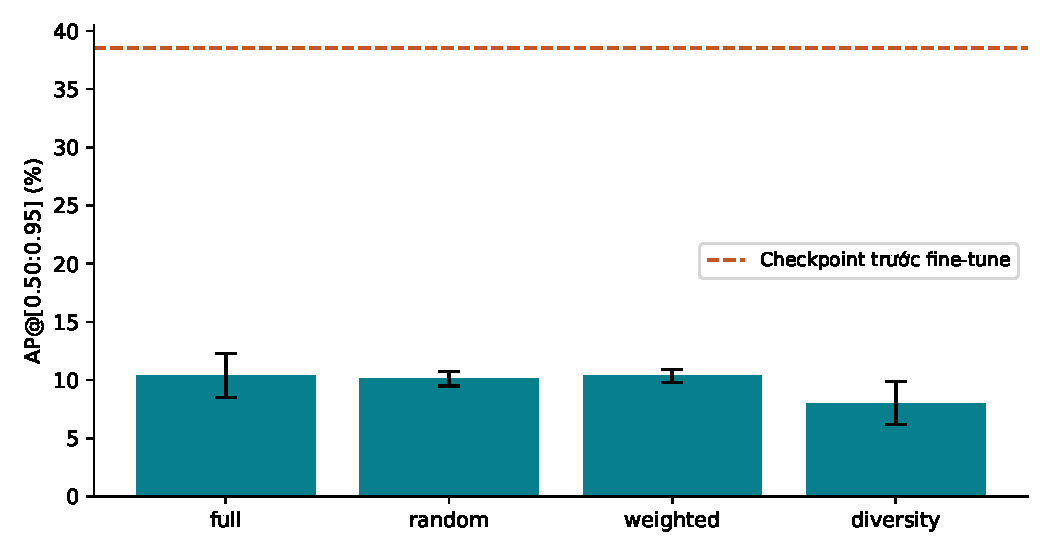
\includegraphics[width=.88\textwidth]{klygo/mining_training.pdf}
\caption{Chất lượng sau fine-tune và checkpoint ban đầu trên cùng tập test}
\end{figure}
Checkpoint ban đầu đạt AP 38.52\% trên cùng 100 ảnh test ở kích thước 320. Weighted chênh +0.28 điểm phần trăm AP so với Random cùng 150 ảnh. Diversity chênh -2.10 điểm phần trăm AP so với Random cùng 150 ảnh. Các chênh lệch là mô tả mẫu; ba seed không đủ để khẳng định khác biệt có ý nghĩa thống kê hoặc ưu thế trên các tập dữ liệu khác. Độ lệch chuẩn phản ánh biến thiên huấn luyện, không phải khoảng tin cậy do lấy mẫu ảnh test.

Thời gian train là thời gian tường của lời gọi train, gồm khởi tạo trainer, lưu checkpoint và xử lý validation bên trong thư viện, không gồm đánh giá test riêng. Đây là so sánh cùng epoch: full có khoảng gấp đôi số batch cập nhật so với mỗi tập con. Chi phí mining cũng cần cộng vào khi xét tổng thời gian. Năm epoch và 100 ảnh test là một thực nghiệm thăm dò; không đủ để xếp hạng phương pháp trên toàn COCO hay suy ra kết quả học từ đầu. Fine-tune ngắn có thể giảm AP so với checkpoint ban đầu do tập nhỏ và thay đổi phân bố; kết quả giảm vẫn được báo cáo.

\section{Benchmark framework gốc và các chế độ Klygo}
\label{sec:execution-exp}
Thực nghiệm dùng YOLOv8n và YOLO-World v2 small ở revision \code{c4388f1}, theo sáu cấu hình đã phân biệt ở Hình~\ref{fig:execution-paths} và bảng tương ứng trong chương thiết kế. Cả sáu nhánh được đo lại trong phiên ngày 07/11/2026; không ghép một hàng mới vào kết quả năm nhánh của phiên trước. Mỗi cặp model/chế độ được nạp trong tiến trình riêng. Đầu vào là cùng 100 ảnh JPEG theo thứ tự manifest, đặt tên để thứ tự duyệt thư mục được xác định. Mỗi nhánh có một lượt warm-up toàn tập rồi ba lượt đo toàn tập; batch một, FP32, kích thước 640, confidence 0,25, IoU 0,7 và max detections 100. Không thay vocabulary YOLO-World.

Lượt thăm dò ở confidence 0,001 dừng tại Klygo native do backend trả box có chiều rộng hoặc chiều cao bằng không, bị validator từ chối. Log và các kết quả Raw của lượt này được giữ riêng, không ghép vào bảng. Benchmark đầy đủ được chạy lại ở confidence 0,25 cho tất cả các nhánh, không loại ảnh gây lỗi. Đây là cấu hình phục vụ suy luận thông thường; chưa chứng minh revision mới hoạt động với mọi box ở ngưỡng rất thấp. Không dùng bảng thời gian này làm thời gian tính AP ở confidence 0,001.

Timer bao gồm giải mã nguồn, suy luận, hậu xử lý và trả kết quả công khai; không gồm nạp trọng số. Với stream, timer kéo dài đến khi tiêu thụ hết iterator. Thời điểm kết quả đầu tiên được quan sát từ phía người gọi, nên ở non-stream/native nó bao gồm chờ hoàn thành collection; không được gọi là độ trễ suy luận của một frame. CUDA được đồng bộ tại ranh giới đo và khi nhận kết quả đầu. Việc chuẩn hóa dự đoán để đối chiếu được thực hiện trong một lượt riêng, ngoài timer.

RAM là RSS đỉnh được lấy mẫu mỗi 10 ms trong tiến trình; VRAM là đỉnh bộ nhớ tensor do PyTorch cấp phát, không phải toàn bộ bộ nhớ thiết bị do trình điều khiển báo. Các cột bộ nhớ là MiB tuyệt đối và có bao gồm model/runtime. Số liệu là trung vị ba lượt. Chênh lệch bộ nhớ so với trước mỗi lượt cũng được lưu trong JSON; phép đo ngắn chưa kiểm chứng giới hạn bộ nhớ của một video kéo dài.

\begin{table}[H]\centering\small
\caption{YOLOv8n: cùng 100 ảnh, các chế độ thực thi}
\begin{tabular}{lrrrrr}
\toprule
Chế độ & Giây & Ảnh/s & Đầu (ms) & RAM & VRAM \\
\midrule
raw & 1.93 & 51.91 & 1926.5 & 1164 & 46 \\
raw stream & 2.14 & 46.77 & 23.7 & 1075 & 46 \\
native & 2.24 & 44.74 & 2235.0 & 1137 & 46 \\
native backend stream & 1.99 & 50.23 & 1990.8 & 1071 & 46 \\
managed & 1.83 & 54.70 & 1828.2 & 1062 & 38 \\
managed stream & 1.99 & 50.26 & 35.1 & 1060 & 38 \\
\bottomrule
\end{tabular}

\end{table}
\begin{table}[H]\centering\small
\caption{YOLO-World: cùng 100 ảnh, các chế độ thực thi}
\begin{tabular}{lrrrrr}
\toprule
Chế độ & Giây & Ảnh/s & Đầu (ms) & RAM & VRAM \\
\midrule
raw & 2.84 & 35.25 & 2836.5 & 1253 & 137 \\
raw stream & 2.60 & 38.47 & 27.2 & 1171 & 137 \\
native & 3.25 & 30.77 & 3250.2 & 1201 & 137 \\
native backend stream & 2.99 & 33.40 & 2994.0 & 1121 & 137 \\
managed & 2.52 & 39.71 & 2518.2 & 1125 & 128 \\
managed stream & 2.54 & 39.33 & 41.9 & 1126 & 128 \\
\bottomrule
\end{tabular}

\end{table}
\begin{figure}[H]\centering
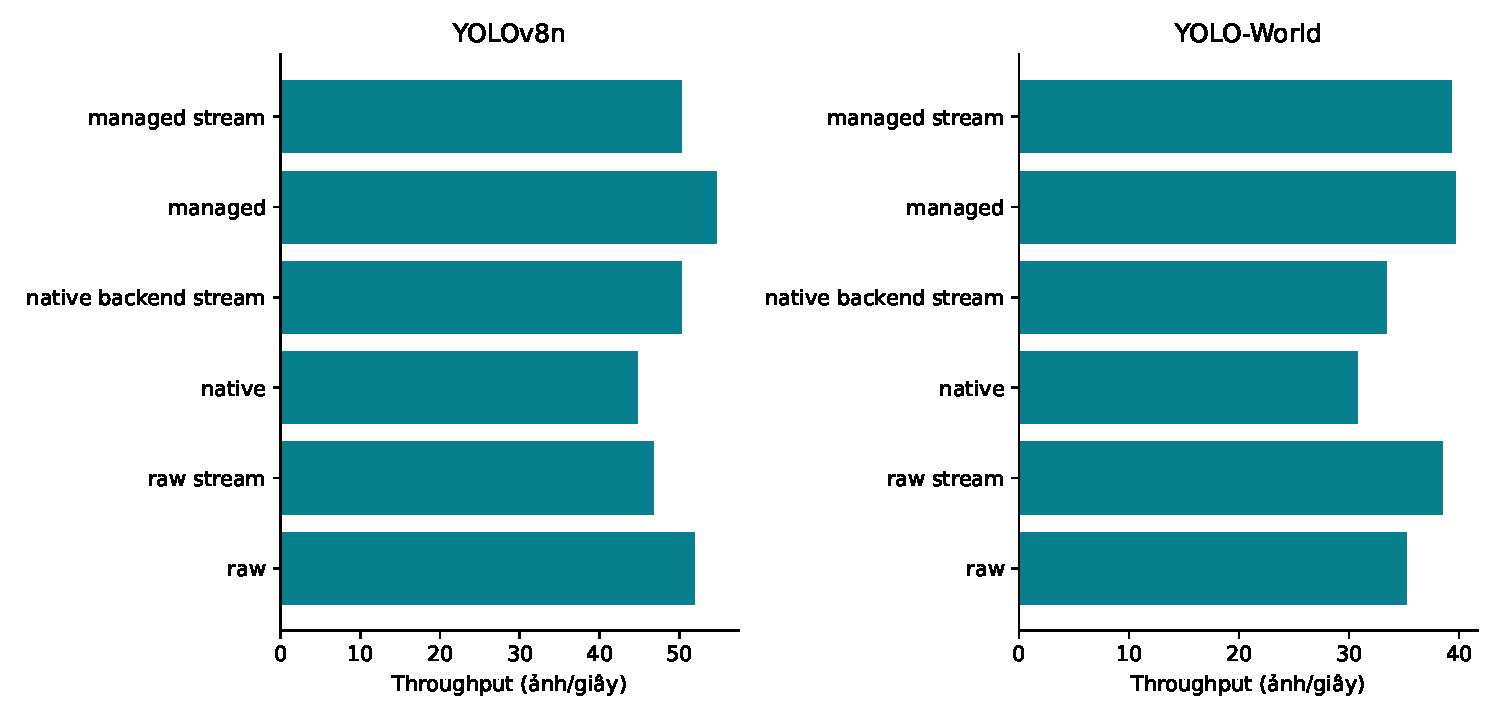
\includegraphics[width=\textwidth]{klygo/execution_throughput.pdf}
\caption{Throughput của framework gốc và các đường thực thi Klygo}
\end{figure}
YOLOv8n: chênh lệch thời gian toàn tập so với Raw là native +16.0\%, native backend stream +3.3\%, managed -5.1\%, managed stream +3.3\%. Dấu dương biểu thị chậm hơn, dấu âm biểu thị nhanh hơn trong phép đo này.

Đối chiếu YOLOv8n có 0/500 cặp frame vượt tiêu chí tương đương: cùng số box, class và sai số tọa độ không quá 0,01 pixel, score không quá 0,001. Sai số lớn nhất theo cách ghép class/score là 0.000000 pixel và 0.000000 điểm score. Phép kiểm tra này dùng dự đoán framework làm tham chiếu, không gọi đó là ground truth.

YOLO-World: chênh lệch thời gian toàn tập so với Raw là native +14.6\%, native backend stream +5.5\%, managed -11.2\%, managed stream -10.4\%. Dấu dương biểu thị chậm hơn, dấu âm biểu thị nhanh hơn trong phép đo này.

Đối chiếu YOLO-World có 0/500 cặp frame vượt tiêu chí tương đương: cùng số box, class và sai số tọa độ không quá 0,01 pixel, score không quá 0,001. Sai số lớn nhất theo cách ghép class/score là 0.000000 pixel và 0.000000 điểm score. Phép kiểm tra này dùng dự đoán framework làm tham chiếu, không gọi đó là ground truth.

Raw trả kiểu dữ liệu của framework, còn Klygo bổ sung container, identity và metadata. Vì đầu ra có chức năng khác nhau, chênh lệch Raw--Klygo là chi phí hoặc lợi ích của đường xử lý hoàn chỉnh, không cô lập thời gian kernel mạng. Native--Managed giúp quan sát thêm ảnh hưởng điều phối nguồn. Không dùng phép đo này để tuyên bố kiến trúc mạng đã được tối ưu, hoặc mọi cấu hình stream đều nhanh hơn non-stream.

Các chế độ được chạy nối tiếp trong những tiến trình khác nhau, chưa hoán đổi thứ tự theo một thiết kế ngẫu nhiên cân bằng. Tải hệ điều hành, cache đĩa và trạng thái nhiệt/xung GPU vẫn có thể tạo nhiễu; ba lượt đo không loại bỏ được các yếu tố đó. Những chênh lệch nhỏ cần được kiểm tra lại trên nhiều phiên đo trước khi xem là cải thiện hiệu suất ổn định.

\section{Ảnh hưởng của worker và prefetch}
\label{sec:scheduling-exp}
Thực nghiệm tiếp theo giữ chế độ Managed stream và cùng toàn bộ cấu hình model, dữ liệu, phần cứng, ngưỡng, warm-up cùng số lượt đo của benchmark sáu mode. Chỉ thay cặp (workers, prefetch), ký hiệu (W,P). Mỗi cấu hình được nạp ở một tiến trình riêng; tham chiếu (1,1) lấy từ Managed stream của cùng phiên đo sáu mode. Không chạy huấn luyện hoặc một benchmark GPU khác đồng thời.

Các cặp được cố định trước khi chạy: (0,0), (1,1), (2,1), (4,1), (2,2), (2,4). Nhánh (0,0) là chuẩn bị tuần tự. Nhóm (1,1), (2,1), (4,1) giữ P=1 để khảo sát số worker; nhóm (2,1), (2,2), (2,4) giữ W=2 để khảo sát độ sâu hàng đợi. Batch vẫn bằng một, nên kết quả chưa đại diện cho khả năng giải mã nhiều ảnh trong cùng một batch lớn.

\begin{table}[H]\centering\small
\caption{YOLOv8n Managed stream: ảnh hưởng của worker/prefetch trên 100 ảnh}
\begin{tabular}{rrrrrrr}
\toprule
W & P & Giây & Min--max (s) & Ảnh/s & Đầu (ms) & RAM \\
\midrule
0 & 0 & 2.05 & 2.01--2.17 & 48.84 & 32.6 & 1060 \\
1 & 1 & 1.99 & 1.86--2.06 & 50.26 & 35.1 & 1060 \\
2 & 1 & 1.98 & 1.88--2.05 & 50.57 & 38.9 & 1063 \\
4 & 1 & 2.17 & 2.08--2.23 & 46.03 & 33.9 & 1073 \\
2 & 2 & 1.83 & 1.83--1.95 & 54.67 & 37.8 & 1063 \\
2 & 4 & 1.82 & 1.81--1.89 & 55.05 & 39.3 & 1063 \\
\bottomrule
\end{tabular}

\end{table}
\begin{table}[H]\centering\small
\caption{YOLO-World Managed stream: ảnh hưởng của worker/prefetch trên 100 ảnh}
\begin{tabular}{rrrrrrr}
\toprule
W & P & Giây & Min--max (s) & Ảnh/s & Đầu (ms) & RAM \\
\midrule
0 & 0 & 2.80 & 2.75--2.87 & 35.76 & 40.8 & 1123 \\
1 & 1 & 2.54 & 2.52--2.57 & 39.33 & 41.9 & 1126 \\
2 & 1 & 2.53 & 2.51--2.55 & 39.55 & 42.0 & 1139 \\
4 & 1 & 2.56 & 2.54--2.74 & 39.03 & 41.2 & 1128 \\
2 & 2 & 2.57 & 2.53--2.61 & 38.93 & 45.9 & 1127 \\
2 & 4 & 2.55 & 2.55--2.56 & 39.27 & 42.3 & 1126 \\
\bottomrule
\end{tabular}

\end{table}
Các cột thời gian toàn tập, throughput, thời gian tới kết quả đầu và RSS đỉnh là trung vị ba lượt; cột min--max là khoảng quan sát của thời gian toàn tập qua ba lượt, không phải khoảng tin cậy. RAM dùng MiB, lấy mẫu 10 ms như phần trước. Các file JSON còn lưu đỉnh VRAM và chênh lệch bộ nhớ so với trước mỗi lượt. RSS phụ thuộc cả model/runtime và allocator, nên không diễn giải mọi chênh lệch RSS thành dung lượng riêng của hàng đợi prefetch.

\begin{figure}[H]\centering
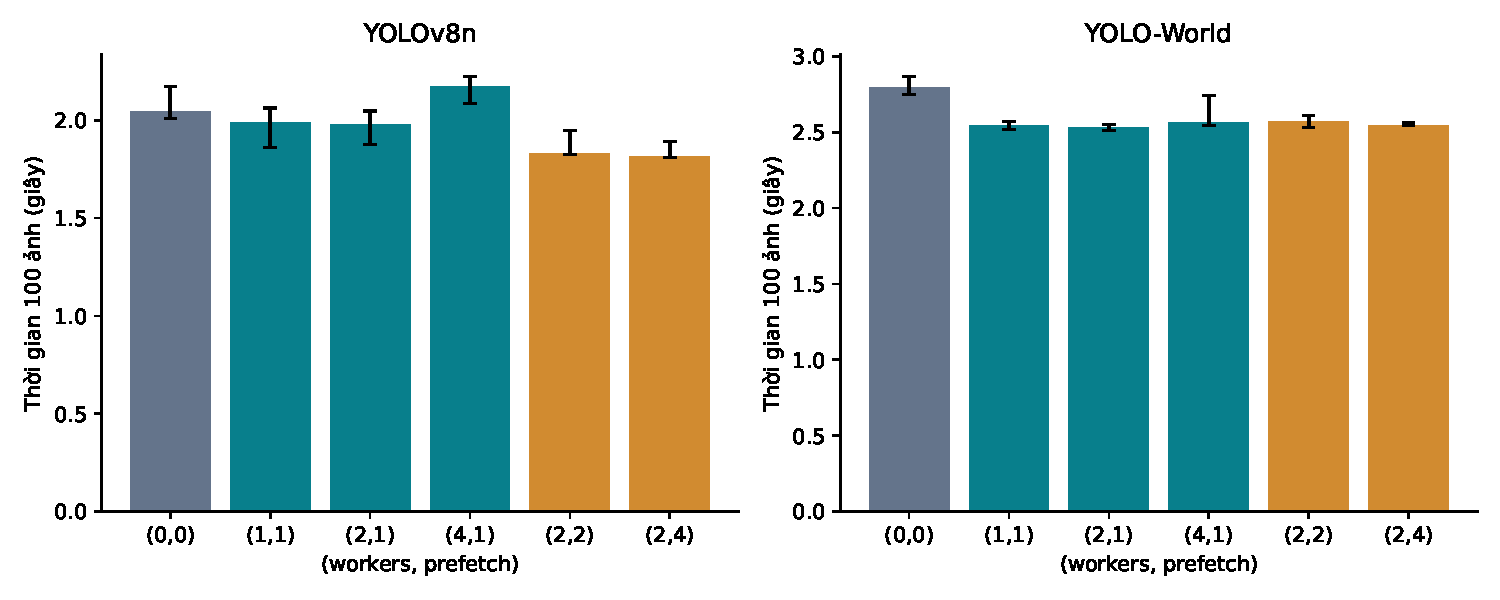
\includegraphics[width=\textwidth]{klygo/scheduling_comparison.pdf}
\caption{Thời gian xử lý theo cặp worker/prefetch; cột là trung vị, thanh sai số biểu diễn min--max của ba lượt}
\end{figure}
YOLOv8n: trung vị nhỏ nhất trong các cấu hình đã đo là (2,4) với 1.82 s; mặc định (1,1) là 1.99 s và tuần tự (0,0) là 2.05 s. Đây là mô tả phiên đo, không khẳng định cấu hình tối ưu trên mọi workload.

Sáu cấu hình YOLOv8n có 0/600 cặp frame vượt tiêu chí tương đương so với Raw, với cùng ngưỡng sai số như benchmark sáu mode.

YOLO-World: trung vị nhỏ nhất trong các cấu hình đã đo là (2,1) với 2.53 s; mặc định (1,1) là 2.54 s và tuần tự (0,0) là 2.80 s. Đây là mô tả phiên đo, không khẳng định cấu hình tối ưu trên mọi workload.

Sáu cấu hình YOLO-World có 0/600 cặp frame vượt tiêu chí tương đương so với Raw, với cùng ngưỡng sai số như benchmark sáu mode.

Chọn cấu hình sử dụng còn phụ thuộc độ trễ chấp nhận được và ngân sách RAM. Tăng worker/prefetch không có cam kết giảm thời gian đơn điệu; lợi ích chỉ xuất hiện khi nó giúp giải mã theo kịp mô hình, trong khi các chi phí đồng bộ và giữ pixel vẫn tồn tại. Phiên đo hữu hạn này chưa đánh giá nguồn video dài, batch lớn hay đọc dữ liệu qua mạng. Vì các cấu hình chưa được chạy theo thứ tự ngẫu nhiên cân bằng, kết quả cần được tái kiểm chứng trước khi dùng làm khuyến nghị triển khai chung.


\chapter{Minh Chứng Sản Phẩm Và Hướng Dẫn Sử Dụng}
\label{chap:demo}
\section{Cài đặt và chuẩn bị}
Sản phẩm trong phạm vi đề tài là một thư viện Python cùng ví dụ và công cụ thực nghiệm, được sử dụng qua chương trình hoặc notebook. Khi chuẩn bị demo, người dùng cần chọn môi trường Python phù hợp, cài package Klygo và backend cần dùng, đồng thời kiểm tra checkpoint và dữ liệu đầu vào. Với thí nghiệm báo cáo, môi trường riêng \code{.venv-report} đã được tạo tại thư mục workspace để tách phụ thuộc khỏi môi trường Python hệ thống.

Cặp PyTorch 2.8.0 và Torchvision 0.23.0 được cài từ kho CUDA 12.6 theo hướng dẫn phiên bản chính thức~\cite{pytorchversions}. Việc cài xong gói không bảo đảm có thể thực thi CUDA; mã demo và thực nghiệm kiểm tra bằng \code{torch.cuda.is\_available()} cùng một phép toán tensor trên thiết bị. Nếu không có CUDA, chương trình thực nghiệm báo lỗi khi cấu hình yêu cầu GPU, thay vì tự đổi sang CPU và giữ nhãn điều kiện đo cũ.

\begin{lstlisting}[language={},caption={Lệnh kiểm tra môi trường và chạy demo từ workspace}]
.venv-report\Scripts\python.exe -m pip check
.venv-report\Scripts\python.exe -X utf8 report\experiments\demo_klygo.py
\end{lstlisting}
Mã demo sử dụng các checkpoint và ảnh đã chuẩn bị. Tệp \code{verification.json} lưu kích thước nguồn, nhãn, số box, thông tin khôi phục và số frame stream đã tiêu thụ. Các lệnh tải và tái lập toàn bộ thực nghiệm được đặt ở phụ lục để phần demo tập trung vào hành vi sử dụng thư viện.

\section{Pipeline phát hiện một ảnh}
Ảnh demo COCO ID 125778 có kích thước $640\times480$. Mã tạo một \code{LazyImage}, gọi Detector, áp dụng pipeline hậu xử lý, rồi vẽ kết quả theo các mảng box, nhãn và score. Trong lần chạy đã lưu, kết quả sau lọc confidence 0,25 có bảy box, gồm các nhãn potted plant, couch, chair và vase. Số box này chỉ mô tả một lần demo; chất lượng nhận dạng được đánh giá ở Chương~\ref{chap:experiments}.

\begin{lstlisting}[caption={Các thao tác chính trong demo đã chạy}]
image = media.LazyImage(source)
result = detector.predict(
    image, threshold=0.25, verbose=False
)
cleaned = post.compose(
    post.clip(), post.threshold(0.25)
)(result)
frame = cleaned[0]
annotated = visual.draw_bboxes(
    image.to_pil(), frame.boxes,
    labels=frame.labels, scores=frame.scores
)
media.save(output_path, annotated, overwrite=True)
\end{lstlisting}

\begin{figure}[H]\centering
\includegraphics[width=0.9\textwidth]{klygo/demo_prediction.png}
\caption{Kết quả chạy demo qua API công khai của Klygo trên ảnh COCO ID 125778. Ảnh minh họa được sinh bởi mã demo, không phải ảnh giao diện ứng dụng web.}
\label{fig:demo}
\end{figure}
Các bước sau model làm việc trên cấu trúc \code{Detection}, nên có thể sử dụng lại khi đổi adapter. Khi đổi model, người dùng vẫn phải kiểm tra vocabulary và tham số phù hợp. Giao diện chung giúp giảm mã chuyển đổi, nhưng không loại bỏ nhu cầu hiểu cấu hình hay chi phí lỗi của bài toán ứng dụng.

\section{Minh họa trace và khôi phục tọa độ}
Demo bổ sung letterbox ảnh $640\times480$ vào khung $640\times640$, tạo padding ở hai phía theo chiều cao. Model dự đoán trên ảnh đã biến đổi; kết quả được gọi \code{restore(target="original")} để liên kết lại với ảnh nguồn và đưa box về không gian $640\times480$. Bản kiểm chứng ghi nhận kích thước khôi phục đúng như ảnh gốc.

\begin{lstlisting}[caption={Khôi phục tường minh sau tiền xử lý hình học}]
transformed = p.compose(
    p.letterbox((640, 640))
)(media.LazyImage(source))
frame = detector.predict(transformed, verbose=False)[0]
restored = frame.restore(target="original")
assert restored.image_size == image.size
\end{lstlisting}
Mã còn tạo box hình học biết trước $[10,20,110,120]$, đưa nó sang hệ tọa độ letterbox bằng scale và padding trong trace, sau đó hoàn tác. Sai số cực đại được kiểm tra nhỏ hơn $10^{-6}$. Phép thử này kiểm chứng phép chuyển đổi tọa độ độc lập với việc model có phát hiện đúng đối tượng hay không. Việc dự đoán trên ảnh letterbox trước model có thể khác dự đoán trực tiếp ảnh gốc, nên demo không ép hai tập dự đoán phải giống nhau.

\section{Suy luận theo stream hữu hạn}
Nguồn thư mục ảnh được đưa vào \code{predict} với \code{stream=True}, \code{max\_frames=6}, \code{batch=2}. Chương trình tiêu thụ iterator và xác nhận nhận đủ sáu frame. Kết quả cho thấy giao diện stream có thể được sử dụng trong một quy trình hữu hạn và các batch được chuyển thành từng frame kết quả.

\begin{lstlisting}[caption={Smoke test stream của thư mục ảnh}]
stream = detector.predict(
    image_folder, stream=True,
    max_frames=6, batch=2, verbose=False
)
frames = list(stream)
assert len(frames) == 6
\end{lstlisting}
Trong lần chạy nguồn thư mục này, thuộc tính \code{frame\_index} được ghi nhận là \code{None}. Thông tin đó được giữ nguyên trong tệp kiểm chứng thay vì tự tạo các chỉ số để làm kết quả đẹp hơn. Người dùng cần dùng đường dẫn ảnh làm định danh cho trường hợp thư mục và kiểm tra hợp đồng chỉ số riêng khi xử lý video. Demo này không phải benchmark bộ nhớ video dài; việc dùng \code{list(stream)} cũng materialize toàn bộ sáu kết quả của smoke test.

\section{Các tình huống lỗi cần xử lý}
\begin{table}[H]\centering\small
\caption{Tình huống lỗi khi cài đặt hoặc sử dụng và hướng xử lý}
\begin{tabularx}{\textwidth}{p{4.2cm}YY}
\toprule Tình huống & Dấu hiệu hoặc nguyên nhân & Hướng xử lý \\\midrule
Thiếu backend tùy chọn & ImportError khi nạp adapter & Cài đúng extra và khóa phiên bản cho môi trường \\
Không có CUDA theo yêu cầu & Kiểm tra thiết bị thất bại & Đổi cấu hình có chủ đích; đo lại và ghi rõ CPU nếu dùng CPU \\
Prompt ngoài vocabulary YOLO & ValueError cho nhãn không hợp lệ & Đối chiếu model.names; dùng model có khả năng mở vocabulary khi phù hợp \\
Box lệch sau resize ngoài model & Nhầm không gian tọa độ & Kiểm tra trace và gọi restore đúng nguồn ảnh \\
Gọi suy luận sau unload & InvalidStateError & Tạo/nạp lại model trước khi dùng \\
Giá trị AP không tương ứng hình demo & Hình đã lọc hoặc chỉ vẽ một phần box & Phân biệt tệp dự đoán đánh giá và cấu hình hiển thị \\
\bottomrule
\end{tabularx}
\end{table}
Quy trình trình bày bảo vệ có thể bắt đầu từ một ảnh, thay adapter, xem cùng kiểu đầu ra, sau đó giải thích manifest và một bảng kết quả. Phần giải thích nên làm rõ dữ liệu nào là ground truth, ngưỡng nào phục vụ hiển thị và ngưỡng nào phục vụ AP. Cách trình bày này giúp kết nối sản phẩm phần mềm với phương pháp đánh giá AI của đề tài.

\clearpage
\section{Tạo bộ dữ liệu bằng mining}
Ví dụ dành cho revision mở rộng, với dataset YOLO đã có ảnh và nhãn:
\begin{lstlisting}[caption={Chọn tập dữ liệu và xuất annotation cùng manifest}]
from klygo import datasets, mining
data = datasets.load("dataset/train", format="yolo")
summary = mining.stats(data)
selected = mining.select(data, method="weighted", limit=150)
mining.compare(data, selected).save("comparison.json")
selected.export("selected_labels", format="yolo")
\end{lstlisting}
Để train, script đọc manifest, sao chép ảnh nguồn sang thư mục images bằng tên tương ứng nhãn và tạo YAML trỏ tới các split. Chương trình \code{run\_mining\_extension.py} thực hiện bước ghép này, kiểm tra đọc lại và lưu ID được chọn. Sau đó \code{prepare\_training\_canonical.py} thống nhất class ID theo tên trên cả train/val/test. Chương trình \code{train\_mining\_extension.py} sử dụng bộ dữ liệu hoàn chỉnh đó, không giả định export tự sao chép ảnh hoặc các registry lớp độc lập có cùng thứ tự.

\chapter{Kết Luận Và Hướng Phát Triển}
\label{chap:conclusion}
\section{Kết quả đạt được}
Đề tài đã mô tả và kiểm chứng revision nền tảng của Klygo với 12 mô-đun và khảo sát revision mở rộng có thêm mining, kết nối quản lý dữ liệu với pipeline phát hiện đối tượng. Cấu trúc BaseModel, Detector, adapter và backend runtime phân chia trách nhiệm giữa phần điều phối dùng chung và xử lý đặc thù framework. Các kiểu Box, Detection và Detections tạo ranh giới đầu ra thống nhất cho hậu xử lý và trực quan hóa.

Trong phạm vi kiểm thử, 353 trong 360 ca đạt và bảy ca được bỏ qua với lý do đã công bố; không có fail hoặc error sau khi cài đủ phụ thuộc. Công cụ audit các mô-đun cũng hoàn tất. Mã demo chạy thật xác nhận luồng ảnh, hậu xử lý, vẽ kết quả, phép hoàn tác tọa độ hình học và một stream hữu hạn. Những bằng chứng này cho thấy các đường đi đã khảo sát có thể vận hành nhất quán, đồng thời không thay thế kiểm chứng cho mọi cấu hình hoặc mọi nguồn dữ liệu.

Thực nghiệm chính đánh giá ba checkpoint pretrained trên cùng 500 ảnh COCO validation. AP lần lượt là \APYolo, \APWorld{} và \APFaster{} cho YOLOv8n, YOLO-World và Faster R-CNN theo cấu hình đã nêu. Độ trễ predict trung bình trong phép đo lặp lần lượt là \LatencyYolo, \LatencyWorld{} và \LatencyFaster{} ms. Những con số này cho phép thảo luận cụ thể sự đánh đổi chất lượng và thời gian thay vì chỉ dựa trên mô tả lý thuyết của kiến trúc.

\section{Trả lời các câu hỏi nghiên cứu}
\textbf{RQ1 -- Giao diện thống nhất.} Klygo đặt hợp đồng chung ở mức nguồn ảnh và kết quả Detection, để adapter dịch dữ liệu riêng của backend. Các mảng box, score, nhãn và class ID được kiểm tra trước khi đóng gói. Cách tổ chức này giúp tái sử dụng hậu xử lý và hiển thị qua nhiều mô hình; vẫn cần adapter đúng để ánh xạ nhãn và tiền xử lý.

\textbf{RQ2 -- Tính đúng của trạng thái và tọa độ.} Snapshot, bản sao metadata, kiểm tra số kết quả theo batch và guard vòng đời giúp hạn chế các lỗi trạng thái. Trace lưu tham số hình học để hoàn tác tọa độ khi người dùng gọi API phù hợp. Đối chiếu mã cho thấy cần sử dụng restore tường minh trong luồng ảnh đã biến đổi, và không nên coi mọi mô tả ``tự động khôi phục'' trong tài liệu là đã được chứng minh cho mọi đường đi.

\textbf{RQ3 -- Chất lượng và độ trễ.} YOLO-World có AP cao nhất trên mẫu nhưng mất thêm thời gian so với YOLOv8n. Faster R-CNN chậm hơn và có AP thấp hơn ở cấu hình giới hạn kích thước đang dùng. Kết quả khác nhau theo lớp và kích thước vật thể; do đó việc chọn cấu hình cần gắn với yêu cầu ứng dụng. Thực nghiệm chưa cung cấp bằng chứng để xếp hạng phổ quát các họ mô hình hoặc các framework.

\textbf{RQ4 -- Chi phí điều phối.} Khi hai nhánh có cùng inference mode, model, ảnh và kết quả Detection, lớp predict bổ sung trung bình khoảng 2,38--2,49 ms so với forward trên phép đo 300 cặp mỗi mô hình. Không ghi nhận khác biệt đầu ra vượt sai số đặt trước. Baseline forward vẫn chứa các thành phần Klygo, nên kết luận chỉ áp dụng cho phần lifecycle và điều phối bổ sung, không phải toàn bộ overhead của thư viện so với framework gốc.

\section{Bài học từ thiết kế và thực nghiệm}
Bài học thứ nhất là phải xác định rõ ranh giới dữ liệu. Sự khác nhau giữa box ID và class ID, chỉ số lớp của từng backend hoặc ảnh gốc và ảnh sau letterbox đều có thể tạo lỗi khó thấy nếu chỉ quan sát chương trình chạy không báo lỗi. Kiểm thử nghiệm hình học và kiểm tra ánh xạ lớp cung cấp bằng chứng trực tiếp hơn cho những ranh giới đó.

Bài học thứ hai là cấu hình và phép đo phải đi cùng kết quả. Một score threshold cao có thể làm hình minh họa gọn hơn nhưng làm mất phần đường cong PR khi tính AP. Một timer không đồng bộ GPU hoặc hai nhánh khác inference context cũng có thể dẫn đến kết luận sai. Việc lưu tệp thô cho phép phát hiện và sửa phương pháp trong khi giữ lại dấu vết các lần thử.

Bài học thứ ba là chuẩn hóa giao diện cần đi kèm công bố các khác biệt còn lại. Cùng tên tham số hoặc cùng kích thước giới hạn không bảo đảm tensor giống nhau. Tương tự, kiểu kết quả tiện dụng có thể thực hiện thêm sao chép, registry và làm tròn. Những lựa chọn đó phục vụ kỹ thuật phần mềm nhưng cần được xét khi dùng thư viện như một công cụ đo chất lượng mô hình.

\section{Hạn chế còn tồn tại}
Mẫu dữ liệu chưa bao phủ đầy đủ phân bố COCO và chưa có benchmark ngoài miền. Một số lớp có ít ground truth; các chênh lệch AP nhỏ chưa được bổ sung khoảng tin cậy. Thực nghiệm chỉ dùng một GPU, batch một và FP32, nên chưa mô tả được khả năng mở rộng hoặc hiệu năng trên thiết bị khác.

Mã builder làm tròn confidence và tọa độ trước khi lưu kết quả; ảnh hưởng định lượng của lựa chọn này chưa được tách riêng. Luồng khôi phục hình học cần được tài liệu hóa thống nhất với cài đặt; nguồn stream thư mục ảnh trong demo revision nền tảng có frame index rỗng; phát hiện này không tự động áp dụng cho revision mở rộng. Các backend Hugging Face và Keras có trong thiết kế nhưng chưa được đánh giá với checkpoint thật ở phép đo chính.

Phần mở rộng đã thực hiện fine-tune ngắn với ba seed; chưa huấn luyện từ đầu, đo năng lượng hay thử tải phục vụ đồng thời. Do vậy báo cáo đóng góp một quy trình thư viện và đánh giá có thể tái lập, không đặt mục tiêu đề xuất kiến trúc học sâu mới hoặc đạt điểm cao nhất trên benchmark.

\section{Hướng phát triển theo mức ưu tiên}
\begin{table}[H]\centering\small
\caption{Hướng phát triển gắn với giới hạn đã quan sát}
\begin{tabularx}{\textwidth}{p{1.2cm}YY}
\toprule Ưu tiên & Công việc & Tiêu chí kiểm chứng \\\midrule
1 & Giữ precision đầy đủ của dữ liệu nội bộ, chỉ làm tròn khi hiển thị & So AP và thứ tự score trước/sau trên cùng dự đoán gốc \\
1 & Đồng bộ tài liệu restore và chỉ số frame với cài đặt & Test nguồn ảnh, thư mục, video và trace qua pipeline công khai \\
2 & Đánh giá toàn bộ validation và bộ dữ liệu ngoài miền & Manifest riêng, cùng protocol; khoảng tin cậy và phân tích theo lớp \\
2 & Bổ sung checkpoint Hugging Face và KerasHub thật & Kiểm tra nhãn, thiết bị, precision và dự đoán theo cùng schema \\
3 & Khảo sát FP16, batch lớn, streaming dài và nhiều thiết bị & Đo chất lượng, độ trễ, bộ nhớ; không chỉ báo FPS \\
3 & Hiệu chuẩn ngưỡng theo ứng dụng & Tập phát triển tách biệt; đánh giá độc lập sau khi chọn ngưỡng \\
\bottomrule
\end{tabularx}
\end{table}
Kết quả của bài tập lớn cho thấy một hệ thống AI có thể được đánh giá thuyết phục khi đi cùng hợp đồng dữ liệu rõ ràng, kiểm thử có mục tiêu và hồ sơ thực nghiệm kiểm tra được. Klygo là nền tảng để nhóm tiếp tục mở rộng quy trình này, với những bước phát triển được dẫn dắt bởi các giới hạn đã quan sát trong mã và số liệu.

\section{Kết luận từ phần mở rộng}
\textbf{RQ5 -- Tuyển chọn dữ liệu.} Mining cung cấp chuỗi đọc, thống kê, chọn, cân bằng và so sánh bộ dữ liệu theo ảnh. Thực nghiệm kiểm chứng dữ liệu sau export và ghép ảnh có thể được đọc lại và dùng fine-tune. Số box và phân bố lớp thay đổi ngay cả khi cùng số ảnh. Kết quả train được báo cáo với ba seed và checkpoint ban đầu làm tham chiếu, không giả định mọi thao tác cân bằng hay phân cụm đều tăng AP.

Trong cấu hình fine-tune năm epoch đã khảo sát, cả bốn tập đều cho AP thấp hơn checkpoint pretrained ban đầu. Kết quả xác nhận khả năng chạy toàn quy trình nhưng chưa chứng minh lợi ích chất lượng của fine-tune này. Weighted gần Random về AP trung bình, còn Diversity thấp hơn; không đủ cơ sở kết luận một phương pháp luôn tốt hơn. Hướng tiếp theo là hiệu chỉnh learning rate, lịch huấn luyện và ngân sách cập nhật bằng tập validation, rồi kiểm chứng một lần trên tập test mới hoặc tập test được giữ kín cho nghiên cứu đó.

\textbf{RQ6 -- Các chế độ thực thi.} Benchmark mới gọi framework gốc trực tiếp, phân biệt sáu cấu hình Raw/native/managed và bổ sung thời gian tới kết quả đầu cùng bộ nhớ. Native với backend stream vẫn thu toàn bộ generator trước khi trả collection trong revision khảo sát; điều này giải thích vì sao không đồng nhất nó với Managed stream. Phép đo worker/prefetch giữ batch cố định và thay từng tham số theo hai nhóm để phân tích chi phí chuẩn bị ảnh. Kết quả chỉ áp dụng cho workload, revision và phần cứng đã đo; khác biệt container và media là một phần chi phí của giao diện công khai. Bằng chứng đối chiếu tọa độ, score và class được lưu riêng ngoài timer.

Hai giới hạn cài đặt đáng lưu ý là Quota/Coverage dùng chung thuật toán ở revision khảo sát, và export chỉ ghi annotation/manifest. Bước ghép ảnh, tạo YAML và huấn luyện do script thực nghiệm đảm nhiệm. Các điểm này giúp mô tả đúng năng lực thư viện, tránh biến tên API hoặc biểu đồ đẹp thành bằng chứng chất lượng mô hình.

\label{page:main-end}
\appendix
\titleformat{\chapter}[display]
  {\normalfont\bfseries\centering\fontsize{16pt}{20pt}\selectfont}
  {PHỤ LỤC \thechapter}{8pt}{\fontsize{16pt}{20pt}\selectfont\MakeUppercase}
\chapter{Phụ Lục Tái Lập Và Đối Chiếu}
\label{chap:appendix}
\section{Cài đặt môi trường}
Các lệnh chạy từ workspace chứa \code{klygo/} và \code{report/}. Môi trường thực nghiệm dùng Python 3.11.9. Cần cài cặp PyTorch/Torchvision phù hợp với thiết bị trước danh sách phụ thuộc đã khóa; cài CUDA wheel không thay thế driver GPU hệ thống.
\begin{lstlisting}[language={},caption={Tạo môi trường riêng và cài đặt phụ thuộc}]
py -3.11 -m venv .venv-report
.venv-report\Scripts\python.exe -m pip install --upgrade pip
.venv-report\Scripts\python.exe -m pip install torch==2.8.0 torchvision==0.23.0 --index-url https://download.pytorch.org/whl/cu126
.venv-report\Scripts\python.exe -m pip install -r report\experiments\requirements.lock.txt
.venv-report\Scripts\python.exe -m pip install -e .\klygo
.venv-report\Scripts\python.exe -m pip check
\end{lstlisting}
Tệp khóa phiên bản ghi các phụ thuộc của môi trường đã sử dụng. Klygo editable được cài riêng để tránh cố định đường dẫn tuyệt đối của máy thí nghiệm. Tiện ích đọc PDF phục vụ kiểm tra báo cáo có thể có trong bản xuất môi trường, nhưng không tham gia timer suy luận.

\section{Chuẩn bị dữ liệu và checkpoint}
\begin{lstlisting}[language={},caption={Tải mẫu ảnh cố định và checkpoint công khai}]
.venv-report\Scripts\python.exe -u report\experiments\prepare_coco.py --image-limit 0 --annotation-json-url https://huggingface.co/datasets/LibreYOLO/coco2017/resolve/main/instances_val2017.json
.venv-report\Scripts\python.exe -X utf8 -u report\experiments\run_pilot.py --prepare-weights
\end{lstlisting}
Script tạo manifest với seed 20261105 và lưu thứ tự 500 image ID. Khi manifest đã tồn tại, nó kiểm tra seed, số mẫu, danh sách ID và checksum annotation để tránh thay đổi tập ảnh ngoài ý muốn. Mỗi ảnh được tải xong mới nhận tên chính thức; tệp tải dở có hậu tố riêng. SHA-256 từng ảnh được lưu trong manifest.

Checkpoint YOLO lấy từ release assets của Ultralytics; Faster R-CNN lấy từ kho trọng số Torchvision. Nguồn đầy đủ được lưu trong \code{configuration.json}. Các checksum định danh đúng tệp được dùng, không chỉ dựa trên tên tệp. SHA-256 của annotation là:
\begin{center}\footnotesize\ttfamily
e8c7f7908f1d7278341fae127d0da654f\\
102f11bd7b21d8aeefa635b8c810b6f
\end{center}
\begin{table}[H]\centering\footnotesize
\caption{SHA-256 của ba checkpoint; mỗi hash được chia hai dòng}
\begin{tabular}{lp{9cm}}
\toprule
Checkpoint & SHA-256 (hai dòng liên tiếp) \\
\midrule
YOLOv8n & \shortstack[l]{\texttt{f59b3d833e2ff32e194b5bb8e08d211d}\\\texttt{c7c5bdf144b90d2c8412c47ccfc83b36}} \\
YOLO-World & \shortstack[l]{\texttt{9b2c17ab6124a913e9b3a5c170617920}\\\texttt{d91b0f01111a8479da69f00e2cf27792}} \\
Faster R-CNN & \shortstack[l]{\texttt{fb6a3cc702b1df54c18a44b26708cd08}\\\texttt{3614211062d0c36d2ca7bf9270df3533}} \\
\bottomrule
\end{tabular}

\end{table}

\section{Lệnh kiểm thử và thực nghiệm}
\label{sec:reproduce}
\begin{lstlisting}[language={},caption={Các lệnh dùng cho kết quả báo cáo}]
.venv-report\Scripts\python.exe -X utf8 report\experiments\check_library.py
.venv-report\Scripts\python.exe -X utf8 report\experiments\test_evaluation.py
.venv-report\Scripts\python.exe -X utf8 -u report\experiments\run_main.py
.venv-report\Scripts\python.exe -X utf8 report\experiments\demo_klygo.py
.venv-report\Scripts\python.exe -X utf8 report\experiments\build_report_assets.py
\end{lstlisting}
\code{run\_main.py} không ghi đè bộ số liệu thời gian đã hoàn tất. Khi chạy mới, nên dùng workspace riêng hoặc một run directory được chỉ định rõ trong mã, giữ nguyên bằng chứng cũ. Nếu đã có dự đoán và metric, có thể sinh lại bảng và hình mà không chạy model một lần nữa.

Audit được chạy từ repository Klygo bằng công cụ \code{.agents/skills/klygo-module-guides/scripts/audit\_public\_api.py --all}. Log và lý do skip nằm trong \code{artifacts/report/logs}. Ba test metric thuộc công cụ báo cáo, không được cộng vào tổng 360 ca hiện có của thư viện.

\section{Tổ chức bằng chứng}
\begin{lstlisting}[language={},caption={Các tệp bằng chứng chính trong artifacts/report}]
data/
  manifest.json
  instances_val2017.json
  instances_sample.json
  images/
weights/
pilot/{yolo,world,faster}/
main/{yolo,world,faster}/
  environment.json
  configuration.json
  predictions.json
  latencies.json
  metrics.json
  diagnostics.json
  cocoeval.txt
  timing_controlled/
    paired_timing.json
    timing_summary.json
demo/
  prediction.png
  verification.json
logs/
  unittest.log
  unittest_summary.json
  api_audit.log
  main_run.log
  controlled_timing.log
\end{lstlisting}
\code{latencies.json} ở thư mục model là thời gian một lượt tạo dự đoán trên 500 ảnh. Bảng thời gian chính lấy từ \code{timing\_controlled}, gồm 100 ảnh và ba lượt đo cặp. Hai tập thời gian có mục đích khác nhau; không ghép chúng để tính trung bình chung.

\code{diagnostics.json} chứa AP theo lớp, đường precision nội suy tại IoU 0,50 và số đếm theo ảnh tại confidence 0,25. \code{summary.json} trong generated tổng hợp dữ liệu cho phần soạn báo cáo. Bảng LaTeX và biểu đồ được tạo từ những bằng chứng này để giảm sai số nhập tay.

\section{Schema dự đoán và tính lại metric}
Dự đoán theo COCO gồm image ID, category ID gốc, box $xywh$ và score. Giá trị được lấy sau chuẩn hóa Klygo, đã chịu quy tắc làm tròn của builder.
\begin{lstlisting}[language={},caption={Schema minh họa; giá trị bên dưới chỉ giải thích trường}]
{
  "image_id": 125778,
  "category_id": 1,
  "bbox": [10.0, 20.0, 100.0, 120.0],
  "score": 0.75
}
\end{lstlisting}
Ví dụ không được dùng như kết quả đo thật của ảnh đó. Để tính lại, nạp annotation, tệp dự đoán và danh sách image ID, đặt \code{iouType="bbox"}, rồi chạy evaluate, accumulate và summarize của COCOeval. Không dùng class ID liên tiếp của model thay category ID COCO nếu chưa đổi ánh xạ đúng cho cả nhãn và dự đoán.

\section{Các ca kiểm thử bỏ qua}
\begin{table}[H]\centering\small
\caption{Bảy ca skip trong suite gốc và lý do}
\begin{tabularx}{\textwidth}{p{4.4cm}p{1.1cm}Y}
\toprule Nhóm & Số ca & Lý do \\\midrule
COCO15: nguồn và 15 lớp & 1 & Chưa sinh dataset từ archive được ghim \\
COCO15: đọc toàn bộ ảnh & 1 & Cùng điều kiện dataset chưa được chuẩn bị \\
COCO15: bundle tái lập & 1 & Chưa tạo bundle theo workflow tương ứng \\
Checkpoint YOLO, YOLO-World & 2 & Chưa đặt biến môi trường cho test opt-in; đã có phép chạy thật riêng trong báo cáo \\
Grounding DINO, Locate Anything & 2 & Chưa cấu hình checkpoint thật; không thuộc phép đo chính \\
\bottomrule
\end{tabularx}
\end{table}

\clearpage
\section{AP theo toàn bộ lớp COCO}
\small\begin{longtable}{lrrrr}
\caption{AP@[0.50:0.95] theo lớp trên mẫu, tính bằng phần trăm; GT không gồm crowd}\label{tab:allclasses}\\
\toprule Lớp & GT & YOLOv8n & YOLO-World & Faster R-CNN \\\midrule\endfirsthead
\toprule Lớp & GT & YOLOv8n & YOLO-World & Faster R-CNN \\\midrule\endhead
person & 1087 & 51{,}20 & 54{,}55 & 32{,}48 \\
bicycle & 32 & 24{,}51 & 37{,}95 & 15{,}43 \\
car & 164 & 33{,}08 & 37{,}25 & 17{,}54 \\
motorcycle & 35 & 29{,}97 & 24{,}93 & 24{,}03 \\
airplane & 23 & 72{,}87 & 72{,}99 & 45{,}09 \\
bus & 42 & 60{,}13 & 69{,}27 & 49{,}80 \\
train & 29 & 65{,}96 & 71{,}64 & 59{,}72 \\
truck & 54 & 26{,}40 & 28{,}14 & 15{,}53 \\
boat & 24 & 14{,}52 & 21{,}59 & 11{,}18 \\
traffic light & 56 & 19{,}75 & 15{,}15 & 10{,}49 \\
fire hydrant & 10 & 53{,}78 & 66{,}15 & 49{,}12 \\
stop sign & 7 & 64{,}16 & 59{,}45 & 59{,}60 \\
parking meter & 3 & 41{,}06 & 6{,}48 & 20{,}84 \\
bench & 25 & 22{,}56 & 25{,}97 & 15{,}29 \\
bird & 49 & 15{,}38 & 19{,}62 & 11{,}23 \\
cat & 19 & 57{,}68 & 48{,}80 & 41{,}74 \\
dog & 13 & 63{,}79 & 61{,}46 & 63{,}23 \\
horse & 17 & 62{,}92 & 58{,}58 & 56{,}95 \\
sheep & 26 & 54{,}99 & 52{,}86 & 45{,}62 \\
cow & 20 & 70{,}94 & 53{,}68 & 53{,}60 \\
elephant & 37 & 66{,}52 & 58{,}73 & 33{,}32 \\
bear & 5 & 48{,}26 & 66{,}31 & 44{,}87 \\
zebra & 19 & 64{,}39 & 69{,}75 & 44{,}25 \\
giraffe & 20 & 87{,}42 & 89{,}67 & 81{,}09 \\
backpack & 31 & 4{,}55 & 18{,}26 & 4{,}18 \\
umbrella & 52 & 46{,}14 & 45{,}67 & 26{,}39 \\
handbag & 58 & 11{,}14 & 20{,}04 & 3{,}23 \\
tie & 32 & 32{,}21 & 35{,}57 & 20{,}81 \\
suitcase & 21 & 17{,}09 & 14{,}71 & 4{,}50 \\
frisbee & 19 & 44{,}21 & 53{,}66 & 17{,}21 \\
skis & 23 & 18{,}02 & 18{,}76 & 8{,}61 \\
snowboard & 5 & 40{,}31 & 34{,}99 & 12{,}56 \\
sports ball & 31 & 30{,}08 & 32{,}26 & 11{,}51 \\
kite & 29 & 43{,}29 & 38{,}59 & 21{,}12 \\
baseball bat & 13 & 41{,}67 & 42{,}24 & 26{,}41 \\
baseball glove & 17 & 53{,}14 & 63{,}85 & 23{,}17 \\
skateboard & 18 & 46{,}12 & 42{,}15 & 43{,}50 \\
surfboard & 19 & 31{,}38 & 33{,}84 & 17{,}89 \\
tennis racket & 20 & 44{,}10 & 47{,}42 & 27{,}87 \\
bottle & 100 & 31{,}59 & 41{,}43 & 16{,}33 \\
wine glass & 24 & 23{,}69 & 37{,}77 & 11{,}67 \\
cup & 83 & 41{,}46 & 46{,}58 & 17{,}59 \\
fork & 11 & 31{,}78 & 29{,}77 & 2{,}41 \\
knife & 20 & 30{,}35 & 29{,}18 & 11{,}78 \\
spoon & 23 & 6{,}40 & 9{,}63 & 1{,}66 \\
bowl & 65 & 40{,}38 & 45{,}70 & 21{,}30 \\
banana & 21 & 30{,}85 & 20{,}22 & 13{,}77 \\
apple & 18 & 25{,}17 & 18{,}63 & 16{,}94 \\
sandwich & 17 & 28{,}47 & 35{,}33 & 26{,}42 \\
orange & 22 & 60{,}45 & 60{,}29 & 41{,}52 \\
broccoli & 23 & 26{,}79 & 19{,}22 & 18{,}02 \\
carrot & 23 & 22{,}32 & 19{,}89 & 9{,}23 \\
hot dog & 20 & 28{,}10 & 20{,}01 & 8{,}45 \\
pizza & 14 & 55{,}29 & 53{,}96 & 47{,}21 \\
donut & 26 & 54{,}15 & 39{,}28 & 10{,}70 \\
cake & 25 & 26{,}54 & 28{,}10 & 11{,}64 \\
chair & 181 & 29{,}19 & 30{,}86 & 15{,}20 \\
couch & 30 & 45{,}44 & 42{,}57 & 26{,}75 \\
potted plant & 43 & 29{,}18 & 36{,}68 & 13{,}24 \\
bed & 22 & 54{,}99 & 47{,}84 & 42{,}31 \\
dining table & 59 & 27{,}34 & 27{,}03 & 17{,}91 \\
toilet & 15 & 51{,}45 & 46{,}84 & 38{,}34 \\
tv & 38 & 46{,}11 & 52{,}00 & 31{,}43 \\
laptop & 27 & 45{,}05 & 50{,}94 & 30{,}71 \\
mouse & 13 & 45{,}40 & 48{,}37 & 39{,}29 \\
remote & 27 & 18{,}27 & 18{,}44 & 12{,}21 \\
keyboard & 17 & 30{,}79 & 36{,}51 & 26{,}70 \\
cell phone & 23 & 28{,}51 & 20{,}36 & 17{,}71 \\
microwave & 5 & 53{,}22 & 60{,}44 & 22{,}75 \\
oven & 16 & 16{,}47 & 12{,}17 & 8{,}09 \\
toaster & 0 & -- & -- & -- \\
sink & 26 & 32{,}63 & 39{,}31 & 16{,}19 \\
refrigerator & 10 & 62{,}18 & 65{,}84 & 52{,}34 \\
book & 80 & 11{,}84 & 11{,}68 & 2{,}27 \\
clock & 33 & 43{,}18 & 45{,}33 & 37{,}62 \\
vase & 33 & 38{,}84 & 43{,}24 & 20{,}17 \\
scissors & 5 & 1{,}46 & 9{,}64 & 10{,}72 \\
teddy bear & 25 & 46{,}13 & 51{,}18 & 33{,}75 \\
hair drier & 1 & 0{,}00 & 0{,}00 & 0{,}00 \\
toothbrush & 7 & 24{,}16 & 21{,}06 & 8{,}19 \\
\bottomrule\end{longtable}\normalsize

``--'' nghĩa là không có ground truth hợp lệ để xác định AP của lớp trong mẫu. Giá trị 0 khác với không xác định: lớp có GT nhưng chưa có kết quả tích lũy đúng theo quy tắc đánh giá. Các lớp có ít GT cần được diễn giải cùng quy mô hỗ trợ.

\section{Biên dịch và chỉnh thông tin nhóm}
Thư mục report dùng XeLaTeX để hỗ trợ Unicode tiếng Việt, phông TeX Gyre Termes và BibTeX cho tài liệu tham khảo. Có thể chọn XeLaTeX trên Overleaf hoặc dùng MiKTeX/TeX Live ở máy cục bộ.
\begin{lstlisting}[language={},caption={Biên dịch thủ công trong thư mục report}]
xelatex -interaction=nonstopmode -halt-on-error main.tex
bibtex main
xelatex -interaction=nonstopmode -halt-on-error main.tex
xelatex -interaction=nonstopmode -halt-on-error main.tex
\end{lstlisting}
Tên đề tài, tên môn, giảng viên và ba dòng thành viên là macro ở đầu \code{main.tex}. Khi chốt họ tên, MSSV và phân công, nhóm cập nhật các macro cùng bảng phân công. Ngày tháng trên bìa là tháng biên soạn, không thay một hạn nộp chính thức chưa được cung cấp.

\section{Tái lập phần mở rộng}
Mã nguồn mở rộng được cố định bằng commit
\begin{center}\small\texttt{c4388f10bba7cf5ff02b9ebc4aa217b9f740e759}\end{center}
Snapshot nằm tại \code{tmp/klygo-c4388f1}; checkout nền tảng giữ nguyên. Tạo snapshot từ bản Git có commit này bằng \code{git archive}, giải nén vào thư mục trên, sau đó chạy theo thứ tự:
\begin{lstlisting}[language={},caption={Lệnh tái lập mining, huấn luyện và benchmark}]
python report/experiments/run_mining_extension.py
python report/experiments/prepare_training_canonical.py
python report/experiments/benchmark_execution.py
python report/experiments/run_scheduling_study.py
python report/experiments/train_mining_extension.py
python report/experiments/check_extension.py
python report/experiments/build_extension_assets.py
python report/experiments/build_scheduling_assets.py
\end{lstlisting}
Không chạy train đồng thời với benchmark suy luận. Dữ liệu, cấu hình, manifest tuyển chọn, bảng đo, dự đoán đối chiếu và kết quả theo seed được lưu dưới \code{klygo/artifacts/report/extension}. Script không ghi đè các kết quả mining đã hoàn tất; các lượt benchmark/train đã có JSON được bỏ qua khi tiếp tục. Muốn thực nghiệm cấu hình mới cần thư mục kết quả mới.

Kiểm thử revision mở rộng chạy 502 ca: 482 đạt, 20 bỏ qua, 0 thất bại và 0 lỗi. Audit trả mã 0. Log đầy đủ nằm trong thư mục extension/checks; số liệu này tách biệt với 360 ca của revision nền tảng.




\clearpage
\phantomsection
\addcontentsline{toc}{chapter}{TÀI LIỆU THAM KHẢO}
\bibliographystyle{ieeetr}
\setlength{\bibsep}{3pt}
\renewcommand{\bibfont}{\small\setstretch{1.0}\raggedright}
\begingroup\small\setstretch{1.0}
\bibliography{klygo_references}
\endgroup
\end{document}
